\documentclass[11pt,a4paper]{book}

\usepackage{lib/Textbook}
\exhyphenpenalty=10000\hyphenpenalty=10000
%\sloppy
\usepackage{enumitem}
\usepackage{mdframed}
\usepackage{tikz}
\usepackage{nccmath}
\usepackage{wrapfig}
\usepackage{textcomp}
\usepackage{multirow}
\usepackage{tasks}
\usetikzlibrary{shapes,arrows,decorations.pathreplacing,calc,positioning,intersections}
\usepackage[export]{adjustbox}
\usepackage{chngcntr}
\usepackage{array}
\usepackage{picture}
\tikzstyle{Box} = [rectangle, minimum height=1cm, draw=black]
\tikzstyle{arrow} = [thick, ->, >=stealth]

\newlist{steps}{enumerate}{1}
\setlist[steps, 1]{label = Step \arabic*:}

\newcommand{\R}{\mathbb{R}}
\newcommand{\N}{\mathbb{N}}
\newcommand{\Z}{\mathbb{Z}}
\newcommand{\Q}{\mathbb{Q}}
\newcommand{\W}{\mathbb{W}}
\newcommand{\C}{\mathbb{C}}

\usepackage{ulem}
\usepackage{graphicx}

\usepackage[english]{babel}
\usepackage{lipsum}
\usepackage{xcolor}
\usepackage{tikz}
\usepackage{mathtools,amsfonts,amssymb,amsthm}
\usepackage[most]{tcolorbox}
\setlength{\parindent}{0pt}

\usepackage{fourier}




\let\cleardoublepage=\clearpage


% Start document
\begin{document}

\tableofcontents

\chapter{Permutations and Combinations}
\section{Basic Counting Principles}

Is a password with at least one uppercase letter really more secure
than one without? What are my odds of winning the lottery? How many
ways could I arrange my friends around the dining table at my dinner
party? In everyday life, we often need to "count"
the number of ways to arrange objects. However listing out all the
possible arrangements is not always easy. In this chapter we will
be learning some fundamental counting techniques, to help us answer
some of life's burning questions.

\subsection{Addition Principle for Counting}

\begin{tcolorbox}[colback=blue!5, colframe=black, boxrule=.4pt, sharpish corners]

The \textbf{Addition Principle for Counting} states that if we have
$a_{1}$ ways of doing something and $a_{2}$ ways of doing another
thing and we cannot do both at the same time, then the number of ways
we can choose $a_{1}$ \textbf{or} $a_{2}$ is
\[
a_{1}+a_{2}
\]
\end{tcolorbox}

Zoe is trying to decide what to wear to the prom. She has 2 ball gowns,
3 blouses and 1 sundress.

How many different outfits can Zoe choose from?

Zoe has $2+3+1=6$ outfits to choose from.

\subsection{Multiplication Principle for Counting}

\begin{tcolorbox}[colback=blue!5, colframe=black, boxrule=.4pt, sharpish corners]

The \textbf{Multiplication Principle for Counting} states that if
there is a sequence of independent events that can occur $a_{1},a_{2},a_{3},...a_{n}$
ways, then the number of ways all the events can occur is
\[
a_{1}\times a_{2}\times a_{3}\times\ldots\times a_{n}
\]
\end{tcolorbox}

Suppose there are three towns $A$, $B$ and $C$ and that four different
roads can be taken from $A$ to $B$ and two different roads from
$B$ to $C$.
\begin{center}
\includegraphics[width=8cm]{\string"lib/Graphics/CountingProductRule\string".png}
\par\end{center}

This begs the question: ``How many different pathways are there from
$A$ to $C$, going through $B$?''

\begin{minipage}[t]{0.5\textwidth}

If we take road 1, there are two different roads to complete our trip.\\

If we take road 2, there are two different roads to complete our trip
... etc.\\

\end{minipage}
\begin{minipage}[t]{0.2\textwidth}
\begin{center}
\includegraphics[width=8cm]{\string"lib/Graphics/CountingProductRule1\string".png}
\par\end{center}

\end{minipage}

So there are $2+2+2+2=4\times2$ different pathways we can take from
$A$ to $C$.

\newpage

Similarly, for
\begin{center}
\includegraphics[width=12cm]{\string"lib/Graphics/CountingProductRule2\string".png}
\par\end{center}

There would be $4\times2\times3=24$ different pathways from $A$
to $D$, passing through $B$ and $C$.

\subsubsection{Lisa's Birthday Party}

Lisa invites six guests to her birthday party: Raj, Alice, Jerry,
Michelle, Ryan and Heather. When they arrive, they shake hands with
each other. Jerry asks: "How many handshakes happened in total?'"

"I shook 6 hands altogether" says
Ryan, "and I guess, so did everybody else.''

"Since there are seven of us, this should mean $7\cdot6=42$ handshakes in total!'' ventures Michelle.

"This seems too many" says Heather.
"The same logic gives 2 handshakes if two persons meet, which is
clearly wrong."

"That is because every handshake was counted twice.
We have to divide $42$ by $2$, to get the right number: $21$."
settles Lisa the issue.

\section{Permutations }

\centerline{\begin{minipage}{.68\textwidth}
\begin{tcolorbox}[colback=blue!5, colframe=black, boxrule=.4pt, sharpish corners]

A \textbf{permutation} is an \textbf{ordered arrangement} of a number
of objects.
\end{tcolorbox}
\end{minipage}}

\medskip

Lisa and her guests make their way to the dining table to eat. Since
it is Lisa's birthday, she sits at the head of the table. How many
different seatings are there (with Lisa\textquoteright s place fixed)?

Let us fill the seats one by one, starting with the chair on Lisa's
right. There are $6$ choices for the guest who will sit down first.
How many choices are there for the guest who goes second? There are
only $5$ choices as the person who went first is already seated.
Therefore there are a total of $6\cdot5$ ways to seat the first two
guests.

We can then proceed in a similar manner: we have $4$ choices for
the third guest to be seated, $3$ choices for the fourth guest to
be seated, and so on. Therefore, the number of ways in which the guests can be seated is
\[
6\cdot5\cdot4\cdot3\cdot2\cdot1=6!=720
\]

\centerline{\begin{minipage}{.58\textwidth}
\begin{tcolorbox}[colback=blue!5, colframe=black, boxrule=.4pt, sharpish corners]

The number of permutations of $n$ different objects is $n!$
\end{tcolorbox}

\end{minipage}}

\begin{example}[Seven Layer Cake]

Alice made a seven layer rainbow cake for Lisa. How many ways could
she have arranged the layers of the cake with the $7$ distinct colours
of the rainbow?

\Solution

The answer is $7!=5040$.

\end{example}

The simplicity of the answer to the this question was due to several
factors: we used each of our objects exactly once, the order of the
objects mattered, and the objects were all different. In the rest
of this section we will study problems without one or more of these
simplifying factors.

\subsection{Permutations Involving Identical Objects}

\begin{example}[Flowers in a Row (Repeated Colours)]

A gardener has five red flowers, three yellow flowers and two white
flowers to plant in a row. In how many different ways can she do that?

\Solution

This problem differs from the previous one in only one aspect: the
objects are not all different. We are going to answer this question
by reducing it to the previous one, in which all objects were different.
Assume our gardener plants her flowers in a row, then sticks labels
(say numbers 1 through 5 for the red flowers, 1 through 3 for the
yellow ones, and 1 through 2 for the white ones) to her flowers so
that she can distinguish them. Now she has ten different flowers,
and therefore the row of flowers she has just finished working on
can look $10!$ different ways. We have to tell how many of these
arrangements differ only because of these labels.

The five red flowers could be given five different labels in $5!$
different ways. The three yellow flowers could be given three different
labels in $3!$ different ways. The two white flowers could be given
two different labels in $2!$ different ways. Therefore, the labeling
of all ten flowers can be done in $5!\cdot3!\cdot2!$ different ways.
Therefore, the total number of arrangements when the labels are removed
is
\[
\frac{10!}{5!\cdot3!\cdot2!}=2520
\]

\end{example}


\medskip{}

\begin{tcolorbox}[colback=blue!5, colframe=black, boxrule=.4pt, sharpish corners]

The number of permutations of $n$ objects with $n_{1}$ identical
objects of the first type, $n_{2}$ identical objects of the second
type, ..., and $n_{k}$ identical objects of the $k$ type is
\[
\frac{n!}{n_{1}!n_{2}!\ldots n_{k}!}
\]
\end{tcolorbox}


\subsection{Permutations Involving Non-Identical Objects}

\subsubsection{Non-Identical Objects Taken Without Repetition}

\begin{example}[20 Politicians Filling 5 Position]

A president must choose five politicians from a pool of 20 candidates
to fill five different cabinet positions. In how many different ways
can she do that?

\Solution

Indeed, we have $20$ choices for the first candidate, $19$ choices
for the second, and so on, just as we did the case of factorials.
The only difference is that here we do not have $20$ slots to fill.
We stop after choosing $5$ of them.

The number $20\cdot19\cdot18\cdot17\cdot16$ is denoted by $^{20}P_{5}$.
Thus, there are $^{20}P_{5}=1860480$ ways of filling this cabinet.
If the candidates are all equally qualified, it may take a while.

\end{example}

\medskip{}

\begin{tcolorbox}[colback=blue!5, colframe=black, boxrule=.4pt, sharpish corners]

The number of permutations of $n$ different objects taken $r$ at
a time \textbf{without repetition} is
\[
^{n}P_{r}=\frac{n!}{\left(n-r\right)!}
\]
\end{tcolorbox}


\subsubsection{Non-Identical Objects Taken With Repetition}

\begin{example}[Building 10 Intersections]

A city has recently built ten intersections. Some of these will get
traffic lights, and some of those that get traffic lights will also
get a gas station. In how many different ways can this happen?

\Solution

For each intersection, there are three possible scenarios:

\begin{enumerate}

\item  No traffic light and no gas station.

\item  Traffic light but no gas station.

\item  Traffic light and a gas station.

\end{enumerate}

Since we have three possible arrangements for each intersection, there
will be $3\cdot3$ possible arrangements for two intersections, and
a total of $3^{10}$ arrangements for the ten intersections to be
built.

\end{example}

\medskip{}

\centerline{\begin{minipage}{.82\textwidth}
\begin{tcolorbox}[colback=blue!5, colframe=black, boxrule=.4pt, sharpish corners]

The number of permutations of $n$ different objects taken $r$ at
a time \textbf{with repetition }is $n^{r}$.
\end{tcolorbox}

\end{minipage}}

\begin{example}[Computer Password]

A certain computer access password consists of 3 through 5 lowercase
letters chosen from the 26 letters in the Roman alphabet, with repetitions
allowed. How many different passwords are possible?

The set of all passwords can be split into three subsets consisting
of passwords with lengths 3, 4, and 5.

By the addition rule, the total number of passwords equals the number
with length 3, plus the number with length 4, plus the number with
length 5.

$\text{Total number of passwords with length 3}=26^{3}$

$\text{Total number of passwords with length 4}=26^{4}$

$\text{Total number of passwords with length 5}=26^{5}$

Hence the total number of passwords is
\[
26^{3}+26^{4}+26^{5}=12355928
\]

(Approximately 12 million)

How many different passwords are possible if the password contains
both uppercase and lowercase letters?

Now instead of having $26$ characters to choose from, we have $52$.

$\text{Total number of passwords with length 3}=52^{3}$

$\text{Total number of passwords with length 4}=52^{4}$

$\text{Total number of passwords with length 5}=52^{5}$

Hence the total number of passwords is
\[
52^{3}+52^{4}+52^{5}=387656256
\]

(Approximately 388 million)

\end{example}

\subsection{Permutations in a Circle }

At a meeting of diplomats, the six participants are to be seated around
a circular table. Since the table has no ends to confer particular
status, it doesn\textquoteright t matter who sits in which chair.
But it does matter how the diplomats are seated relative to each other.
In other words, two seatings are considered the same if one is a rotation
of the other. How many different ways can the diplomats be seated?

Call the diplomats by the letters $A$, $B$, $C$, $D$, $E$, and
$F$. Since only relative position matters, you can start with any
diplomat (say, $A$), place that diplomat anywhere. There is only
one way to do this. Then consider all arrangements of the other diplomats
around that one. The five diplomats $B$ through $F$ can be arranged
in the seats around diplomat $A$ in all possible orders. So there
are $5!=120$ ways to seat the group.

\begin{minipage}{.5\textwidth}
\begin{center}
\includegraphics[width=3.3cm,valign=t]{\string"lib/Graphics/Diplomatsinacircle\string".png}
\par\end{center}

\end{minipage}
\begin{minipage}{.5\textwidth}

Five other diplomats to be seated: $B,C,D,E,F$

\end{minipage}

\medskip

If the seats where numbered/labelled/distinct from each other in some
way, then it would matter what seat they were sitting in and there
would be $n!$ ways of arranging the diplomats.

\medskip

\centerline{\begin{minipage}{.78\textwidth}
\begin{tcolorbox}[colback=blue!5, colframe=black, boxrule=.4pt, sharpish corners]

The number of ways of arranging $n$ different objects in a circle
is $\left(n-1\right)!$
\end{tcolorbox}

\end{minipage}}

\medskip

Unless specified otherwise, all seats are assumed to be not numbered
when circular arrangement is involved.

\begin{example}[Circular Permutations]

\begin{minipage}[t]{.6\textwidth}

How many ways can four friends use their left hands to hold another
friend as shown in the diagram?

\end{minipage}
\begin{minipage}[t]{.38\textwidth}
\begin{center}
\includegraphics[width=4cm,valign=t]{\string"lib/Graphics/4FriendsHandCircle\string".png}
\par\end{center}

\end{minipage}

\Solution

$\text{Number of ways}=\left(4-1\right)!=3!=6$

\end{example}



\newpage{}

\section{Combinations }

\centerline{\begin{minipage}{.89\textwidth}
\begin{tcolorbox}[colback=blue!5, colframe=black, boxrule=.4pt, sharpish corners]

A \textbf{combination} is a selection of objects \textbf{without regard
to order or arrangement}.
\end{tcolorbox}
\end{minipage}}

How many combinations of 3 letter strings can be taken from the set
of 4 letters $\left\{ A,B,C,D\right\} $?

There are $4$ combinations: $ABC$, $BCD$, $ABD$, $ACD$.

\begin{tcolorbox}[colback=blue!5, colframe=black, boxrule=.4pt, sharpish corners]

The number of combinations of $n$ different objects taken $r$ at
a time is
\[
^{n}C_{r}=\begin{pmatrix}n\\
r
\end{pmatrix}=\frac{n!}{r!\left(n-r\right)!}
\]
\end{tcolorbox}

How many ways are there of choosing 5 cards out of a standard $52-$card deck?

The answer is that there are $^{52}C_{5}=2598960$ ways.

\begin{example}[Probability of Winning The Lottery]

In a lottery $5$ numbers are selected from $90$. If George buys
$100$ tickets, what is the probability that he wins?

\Solution

$\text{Total number of combinations}={}^{90}C_{5}=43,949,268$

\begin{align*}
\text{P}\left(\text{George wins}\right) & =\frac{100}{43949268}\\
 & =2.28\times10^{-6}
\end{align*}

\end{example}

\begin{example}[Forming a Team]

The tennis team comprises 8 boys and 12 girls. Three boys and two
girls are to be chosen at random to enter a competition. In how many
ways can this be done?


\Solution


$\text{Number of ways to choose 3 boys}={}^{8}C_{3}$

$\text{Number of ways to choose 2 girls}={}^{12}C_{2}$

Therefore, the total number of ways to choose 3 boys and 2 girls is
$^{8}C_{3}\times{}^{12}C_{2}=3696$.


\end{example}

\begin{example}[Filling Up Seats]

In how many ways can 5 people be chosen to occupy 3 seats in a row?

\Solution

$\text{Number of ways}={}^{5}C_{3}\times3!=60$

Alternatively, $\text{Number of ways}={}^{5}P_{3}=60$
\end{example}


Note:
\begin{itemize}
\item $^{n}P_{r}={}^{n}C_{r}\times r!$
\item $^{n}C_{r}={}^{n}C_{n-r}$
\item $^{n}C_{0}={}^{n}C_{n}=1$
\end{itemize}

\newpage

\begin{example}[Forming a Team With Restrictions]

Suppose a group of twelve consists of five men and seven women.


\begin{enumerate}[label=(\alph*)]

\item How many five-person teams can be chosen that consist of three
men and two women?

\item How many five-person teams contain at least one man?

\item How many five-person teams contain at most one man?

\end{enumerate}

\Solution


\begin{enumerate}[label=(\alph*)]

\item  There are $^{5}C_{3}$ ways to choose $3$ men and $^{7}C_{2}$
ways to choose two women.

Hence by the multiplication rule,

$
\begin{aligned}[t]
\text{Number of teams} & =^{5}C_{3}\times{}^{7}C_{2}\\
 & =210
\end{aligned}
$

\item
$
\begin{aligned}[t]
&\text{Number of teams with at least one man}\\
&=\text{Total number of teams}-\text{Number of teams with no men}\\
&=^{12}C_{5}-{}^{7}C_{5}\\
&=771
\end{aligned}
$

\item
$
\begin{aligned}[t]
&\text{Number of teams with at most one man}\\
&=\text{Number of teams with no men}+\text{Number of teams with one man}\\
 & =^{5}C_{0}\times{}^{7}C_{5}+{}^{5}C_{1}\times{}^{7}C_{4}\\
 & =196
\end{aligned}
$

\end{enumerate}

\end{example}

\newpage


\section{Grouping Method, Inserting Method, Complementary Method}

\begin{example}[Sitting in a Row With Restrictions]

In how many ways can 4 boys and 3 girls be arranged in a row,

\begin{enumerate}[label=(\alph*)]

\item  so that the 3 girls are always together?

\item  so that the first and last place are occupied by boys?

\item  if all the girls are to be separated?

\item  if the 3 girls are not all together together?

\end{enumerate}

\Solution

\begin{enumerate}[label=(\alph*)]

\item  We can put the $3$ girls together as $1$ group.

The number of ways to arrange the $4$ boys and 1 group of girls is
$5!$.

The number of ways the $3$ girls can arrange each other among themselves
is $3!$.

Thus, the total number of ways that the $3$ girls are always together
is $5!\times3!=720$.

(We call this the \textbf{grouping method})

\item  \uline{4} \_ \_ \_ \_ \_ \uline{3}

The $1\text{st}$ and last place can be filled in $3\times4=12$ ways.

The remaining 5 people can be arranged in $5!$ ways.

Thus, the total number of ways the first and last place are occupied
by boys is $12\cdot5!=1440$.

(Alternatively, we could use $\left[^{4}C_{2}\times2!\right]\times5!=1440$)

\item  Here we use the \textbf{slotting method}.

\_$B_{1}$\_$B_{2}$\_$B_{3}$\_$B_{4}$\_

Boys can arrange themselves in $4!$ ways.

There are $5$ slots for the $3$ girls. The girls can arrange themselves
$^{5}C_{3}\times3!=60$ ways.

Thus, the total number of ways that the girls are seperated is $4!\times60=1440$.

\item  Since for any arrangement, EITHER all the 3 girls are together,
OR not all the 3 girls are together,

\begin{align*}
\text{Number of ways 3 girls not all together} & =\text{Total}-\text{Complement}\\
 & =7!-720\quad\text{(From part a)}\\
 & =4320
\end{align*}

(This is known as the \textbf{complementary method})

\end{enumerate}

\end{example}

\newpage

\begin{example}[Sitting Around a Round Table With Restrictions]

4 boys and 3 girls are to be seated at a round table. Andrew, Jane
and Bob are 3 particular people among the 7. How many arrangements
are there if

\begin{enumerate}[label=(\alph*)]

\item there is no restriction?

\item Andrew and Jane must be together?

\item Andrew and Jane must be separated?

\item Jane must sit between Andrew and Bob?

\end{enumerate}

How many arrangements are there if there is no restriction, but the
seats are numbered?

\Solution

\begin{enumerate}[label=(\alph*)]

\item  $\text{Number of arrangements}=\left(7-1\right)!=6!=720$

\item  Group Andrew and Jane together as 1 unit.

$\text{Number of ways to arrange 6 units}=5!$

$\text{Number of internal arrangements for Andrew and Jane}=2!$

$
\begin{aligned}[t]
\text{Number of arrangements} & =5!\times2!\\
 & =240
\end{aligned}
$

\item \begin{minipage}[t]{.6\textwidth}

Use the slotting method.

$\text{Number of ways to arrange other 5 people}=\left(5-1\right)!=4!$

$\text{Andrew and Jane can arrange themselves in }{}^{5}C_{2}\times2!$ ways.

$
\begin{aligned}[t]
\text{Number of arrangements} & =4!\times{}^{5}C_{2}\times2!\\
 & =480
\end{aligned}
$

\end{minipage}
\begin{minipage}[t]{.4\textwidth}
\begin{center}
\includegraphics[width=5cm,valign=t]{\string"lib/Graphics/SlottingMethodCircle\string".png}
\par\end{center}

\end{minipage}

\item  Consider Andrew Jane and Bob as 1 unit.

$\text{Number of ways to arrange 5 units}=4!$

Andrew and Bob can permute among themselves in $2!$ ways.

$
\begin{aligned}
\text{Number of arrangements} & =4!\times2!\\
 & =48
\end{aligned}
$

\end{enumerate}

If seats are numbered, it is equivalent to arranging them in a row.

Therefore, $\text{number of arrangements}=7!=5040$.

\end{example}

\newpage

\begin{example}[Boys and Girls Alternating]

In how many ways can 5 boys and 5 girls be arranged in a row such
that the boys and girls alternate?

\Solution

\begin{enumerate}[label=Case \arabic*:,leftmargin=1.5cm]

\item The first person is a boy. \hspace{1cm}$BGBGBGBGBG$

$\text{Number of ways}=5!\times5!$

\item The first person is a girl. \hspace{1cm}$GBGBGBGBGB$

$\text{Number of ways}=5!\times5!$

\end{enumerate}

Hence, $\text{total number of ways}=5!\times5!+5!\times5!=28800$

\end{example}

\section{Combinations, Pascal\textquoteright s Triangle and The Binomial Distribution}
\begin{center}
\textit{Mathematics is the art of giving the same name to different
things.}
\par\end{center}

\begin{flushright}
-Henri Poincaré\hspace{1cm}
\par\end{flushright}

Pascal's triangle consists of a triangle of numbers where each term
is equal to the sum of the two terms above it. We adopt the convention
that the topmost row is row $0$ and the leftmost term of each row
is the $0\text{th}$ term. It turns out that the $r\text{th}$ term
in the $n\text{th}$ row is given by $^{n}C_{r}$. Try to verify this
for yourself for a few of the terms!

\begin{center}
\def\N{8}
\tikz[x=0.75cm,y=0.5cm,
   pascal node/.style={font=\footnotesize},
   row node/.style={font=\footnotesize, anchor=west, shift=(180:1)}]
  \path
      \foreach \n in {0,...,\N} {
       (-\N/2-1, -\n) node  [row node/.try]{$n=$ \n:}
        \foreach \k in {0,...,\n}{
          (-\n/2+\k,-\n) node [pascal node/.try] {%
            \pgfkeys{/pgf/fpu}%
            \pgfmathparse{round(\n!/(\k!*(\n-\k)!))}%
            \pgfmathfloattoint{\pgfmathresult}%
            \pgfmathresult%
          }}};
\end{center}

The following equations are the binomial expansion of $\left(1+x\right)^{n}$,
where $n=0,1,2,3,4,5,6$.

\begin{align*}
\left(1+x\right)^{0} & =1\\
\left(1+x\right)^{1} & =1+x\\
\left(1+x\right)^{2} & =1+2x+x^{2}\\
\left(1+x\right)^{3} & =1+3x+3x^{2}+x^{3}\\
\left(1+x\right)^{4} & =1+4x+6x^{2}+4x^{3}+x^{4}\\
\left(1+x\right)^{5} & =1+5x+10x^{2}+10x^{3}+5x^{4}+x^{5}\\
\left(1+x\right)^{6} & =1+6x+15x^{2}+20x^{3}+15x^{4}+6x^{5}+x^{6}
\end{align*}

Notice that the coefficients of the binomial expansion of $\left(1+x\right)^{n}$
are simply $\begin{pmatrix}n\\
0
\end{pmatrix},\begin{pmatrix}n\\
1
\end{pmatrix},\begin{pmatrix}n\\
2
\end{pmatrix},\ldots\begin{pmatrix}n\\
n
\end{pmatrix}$.

\newpage

\begin{testyourself}{TEST YOURSELF}
\begin{tasks}[label=(\alph*),label-width=3.5ex]

\task  A permutation is an \rule{4cm}{0.5pt} of a number of objects.

\task  The number of permutations of a set of $n$ elements equals
\rule{2cm}{0.5pt}.

\task  How many ways can the letters in the word COMPUTER be arranged
in a row?

\task  The number of permutations of $n$ different objects taken
$r$ at a time without repetition\textbf{ }is \rule{2cm}{0.5pt}.

\task  A father has 5 books and wishes to give one to each of his
3 children. In how many ways can he do this?

\task  The number of permutations of $n$ different objects taken
$r$ at a time with repetition\textbf{ }is \rule{2cm}{0.5pt}.

\task  How many $3-$digit numbers can be formed from the set $\left\{ 1,2,3,4,5\right\} $
if the digits may be used more than once?

\task  How many ways can we arrange 2 identical white balls and 3
identical red balls in a row?

\task  How many ways can $n$ people sit at a round table?

\task  How many ways can $n$ people sit at a round table if the
seats are numbered?

\task  A combination is a selection of objects without regard to
\rule{4cm}{0.5pt}.

\task  The formula for $^{n}C_{r}$ is \rule{2cm}{0.5pt}.

\task How many ways can we select $5$ people for a team from a group
of 12.

\end{tasks}
\end{testyourself}


\begin{testyourself}{ANSWER}
\begin{tasks}[label=(\alph*),label-width=3.5ex]

\task  A permutation is an \textbf{ordered arrangement} of a number of objects.

\task  The number of permutations of a set of $n$ elements equals
$\boldsymbol{n!}$.

\task  COMPUTER can be arranged $\boldsymbol{8!=40320}$ ways.

\task  The number of permutations of $n$ different objects taken
$r$ at a time without repetition\textbf{ }is $\boldsymbol{
^{n}P_{r}=\frac{n!}{\left(n-r\right)!}}$.

\task  The father can distribute the books $\boldsymbol{^{5}P_{3}=60}$ ways.

\task  The number of permutations of $n$ different objects taken
$r$ at a time with repetition\textbf{ }is $\boldsymbol{n^{r}}$.

\task  From the set $\left\{ 1,2,3,4,5\right\}$, we can form $\boldsymbol{5^{3}=125}$ $3-$digit numbers.

\task  We can arrange 2 identical white balls and 3 identical red balls $\boldsymbol{\frac{5!}{2!\times3!}=10}$ ways.

\task  $n$ people can sit around a table in $\boldsymbol{(n-1)!}$ ways.

\task  If the seats are numbered, they can sit in $\boldsymbol{n!}$ ways.

\task  A combination is a selection of objects without regard to
 \textbf{order or arrangement}.

\task  The formula for $^{n}C_{r}$ is $\boldsymbol{\frac{n!}{r!\left(n-r\right)!}}$.

\task We can select 5 people from a group of 12 in  $\boldsymbol{^{12}C_{5}=792}$ ways.

\end{tasks}
\end{testyourself}

\chapter{Probability}

\section{Gambling and Probability}

Gambling is the wagering of money or something of value on an event
with an uncertain outcome, with the primary intent of winning money
or material goods. The passion for gambling is as old as humanity
itself. In places such as China, Egypt, Greece, Rome, there are evidences that date back to thousands of years ago. Dice games date back to 500BC in ancient rome. Playing cards were found in China as early as the 9th Century during the Tang Dynasty. The first casinos opened in Italy in the 17th century, the first ever being the Casino di Venezia in 1638.

Mans love for gambling is what led the way for the early developments
in probability theory. We wanted to make more money when gambling,
so we searched for optimal gambling strategies. Many developments
in probability theory were stimulated by solving gambling problems
such as
\begin{itemize}
\item De Mere's problem
\item Newton - Pepys problem
\item The St. Petersberg Paradox
\end{itemize}

These days, the magic of gambling has somewhat dissipated. There is
no more uncertainty in the games of chance we play. Whether it is
blackjack, roulette, or slot machines; one thing is for sure: in the
long run, the house always wins. The gambler will inevitably fall
victim of the law of large numbers.

\newpage

\section{Introduction to Probability}

Probability is a measure of chance. In the case where an experiment
has finitely many outcomes and all outcomes are equally likely to
occur, the probability of an event (set of outcomes) is just the ratio
of the number of outcomes in the event to the total number of outcomes
(which we call the sample space).

\medskip

\centerline{\begin{minipage}{.88\textwidth}
\begin{tcolorbox}[colback=blue!5, colframe=black, boxrule=.4pt, sharpish corners]

A \textbf{sample space} is the set of all possible outcomes of a random
process or experiment.

\medskip

An \textbf{event} is a subset of a sample space.
\end{tcolorbox}
\end{minipage}}

\medskip

For example, a fair six-sided die has a sample of $S=\left\{ 1,2,3,4,5,6\right\} $.

$\therefore n\left(S\right)=6$

Suppose $E$ is the event that an even number is rolled. Since the
even numbers in $S$ are $2,4,6$, event $E$ can be written as $E=\left\{ 2,4,6\right\} $.

$\therefore n\left(E\right)=3$

\medskip

\begin{tcolorbox}[colback=blue!5, colframe=black, boxrule=.4pt, sharpish corners]

If $S$ is a finite sample space in which all outcomes are equally
likely and $E$ is an event in $S$, then the probability of $E$,
denoted $\text{P}\left(E\right)$, is
\[
\text{P}\left(E\right)=\frac{\text{the number of outcomes in }E}{\text{the total number of ountcomes in }S}
\]
\end{tcolorbox}

\medskip

We can thus find that the probability of event $E$, rolling an even
number on a die, is
\[
\text{P}\left(E\right)=\frac{n\left(E\right)}{n\left(S\right)}=\frac{3}{6}=\frac{1}{2}
\]

\begin{itemize}
\item For any event $E$, $0\leq\text{P}\left(E\right)\leq1$.
\item If $E$ is an impossible event, then $\text{\text{P}\ensuremath{\left(E\right)}}=0$,
i.e. it will never occur.
\item If $E$ is an certain event, then $\text{P}\left(E\right)=1$, i.e.
it will definitely occur.
\item If $E$ is any event, then $\text{P}\left(E\right)=1-\text{P}\left(E'\right)$,
where $\text{P}\left(E'\right)$ is the probability that $E$ does
not occur.
\end{itemize}
\setlength{\extrarowheight}{6pt}

\begin{flushright}

\tcbox[box align=base,nobeforeafter,colback=white, colframe=black, sharp corners]{
\begin{minipage}[t]{.53\textwidth}
\begin{tabular}{>{\centering}p{2cm}|>{\raggedright}p{5.5cm}}
\textbf{Notations} & \textbf{What it means}\tabularnewline
\hline
$A\cup B$ & Union of $A$ and $B$\tabularnewline
\hline
$A\cap B$ & Intersection of $A$ and $B$\tabularnewline
\hline
$\in$ & ``... is an element of ...''\tabularnewline
\hline
$\not\in$ & ``... is not an element of ...''\tabularnewline
\hline
$n\left(A\right)$ & Number of elements in set $A$\tabularnewline
\hline
$A'$ & Complement of set $A$\tabularnewline
\hline
$\text{Ø}$ & Empty set or null set\tabularnewline
\hline
$\xi$ & Universal set\tabularnewline
\hline
$A\subseteq B$ & $A$ is a subset of $B$\tabularnewline
\hline
$A\subset B$ & $A$ is a proper subset of $B$\tabularnewline
\hline
$A\not\subseteq B$ & $A$ is not a subset of $B$\tabularnewline
\hline
$A\not\subset B$ & $A$ is not a proper subset of $B$\tabularnewline
\end{tabular}

\end{minipage}}
\par\end{flushright}


\newpage
\section{Venn Diagrams}

A Venn diagram consists of a universal set $\xi$ represented by a
rectangle. Sets within the universal set are represented by circles.

\textbf{\large{}Subset}{\large\par}

If $B\subseteq A$ then every element of $B$ is also in $A$. The
circle representing $B$ is placed within the circle representing
$A$ and does not leave its boundaries.
\begin{center}
\includegraphics[width=5cm]{\string"lib/Graphics/VennD7\string".png}
\par\end{center}

\textbf{\large{}Intersection}{\large\par}

$A\cap B$ consists of all elements common to both $A$ and $B$.
It is the shaded region where the circles representing $A$ and $B$
overlap.
\begin{center}
\includegraphics[width=5cm]{\string"lib/Graphics/VennD1\string".png}
\par\end{center}

\textbf{\large{}Union}{\large\par}

$A\cup B$ consists of all elements which are in $A$ or $B$. It
is the shaded region which includes both circles.
\begin{center}
\includegraphics[width=5cm]{\string"lib/Graphics/VennD2\string".png}
\par\end{center}

\textbf{\large{}Disjoint or Mutually Exclusive}{\large\par}

Disjoint sets do not have common elements. They are represented by
non-overlapping circles.
\begin{center}
\includegraphics[width=5cm]{\string"lib/Graphics/VennD6\string".png}
\par\end{center}

\textbf{\large{}Complement}{\large\par}
$A'$ is called the complement of $A$. It is the shaded region which includes everything except the set $A$.
\begin{center}
\includegraphics[width=5cm]{\string"lib/Graphics/VennD9\string".png}
\par\end{center}


\newpage

\section{Independent Events}

\centerline{\begin{minipage}{.70\textwidth}
\begin{tcolorbox}[colback=blue!5, colframe=black, boxrule=.4pt, sharpish corners]

\textbf{Independent events} are events where the occurrence of one
of the events \textbf{does not} affect the occurrence of the other
event.
\end{tcolorbox}
\end{minipage}}

\medskip

For example, if a coin and a die are tossed simultaneously, there
is no way that the outcome of one will affect the outcome of the other.
Thus, the two events ``getting a heads'' and ``rolling a six''
are independent events.

\medskip

\centerline{\begin{minipage}{.75\textwidth}
\begin{tcolorbox}[colback=blue!5, colframe=black, boxrule=.4pt, sharpish corners]

If $A$ and $B$ are \textbf{independent events} then $\text{P}\left(A\textbf{ and }B\right)=\text{P}\left(A\right)\times\text{P}\left(B\right)$
\end{tcolorbox}
\end{minipage}}

\begin{example}[Determining Whether Events are Independent]

Two ordinary fair dice, one red and one blue, are thrown. Events $A$,
$B$ and $C$ are defined as follows:

Event $A$: the number showing on the red die is 5 or 6

Event $B$: the total of the numbers showing on the two dice is 7

Determine whether events $A$ and $B$ are independent.

\Solution

$
\begin{aligned}[t]
\text{P}\left(A\right) & =\frac{2}{6}\\
 & =\frac{1}{3}
\end{aligned}
$
\hspace{2cm}
$
\begin{aligned}[t]
\text{P}\left(B\right) & =\frac{6}{36}\\
 & =\frac{1}{6}
\end{aligned}
$
\hspace{2cm}
$
\begin{aligned}[t]
\text{P\ensuremath{\left(A\cap B\right)}} & =\frac{2}{36}\\
 & =\frac{1}{18}
\end{aligned}
$

Since ${\displaystyle \text{P}\left(A\cap B\right)=\text{P}\left(A\right)\times\text{P}\left(B\right)=\frac{1}{18}}$,
therefore $A$ and $B$ are independent.
\end{example}

\section{Dependent Events}

Suppose a hat contains $4$ red and $2$ blue tickets. One ticket
is randomly chosen, its colour is noted and it is thrown in a bin.
A second ticket is randomly selected. What is the chance that it is
red?

If the first ticket was red, ${\displaystyle \text{P(second is red)}=\frac{3}{5}}$

If the first ticket was blue, ${\displaystyle \text{P(second is red)}=\frac{4}{5}}$

So, the probability of the second ticket being red \textbf{depends}
on what colour the first ticket was. Here we have \textbf{dependent
events}.

\medskip

\centerline{\begin{minipage}{.65\textwidth}
\begin{tcolorbox}[colback=blue!5, colframe=black, boxrule=.4pt, sharpish corners]

\textbf{Dependent events} are events where the occurrence of one of
the events\textbf{ does} affect the occurrence of the other event.
\end{tcolorbox}
\end{minipage}}

\newpage

\section{Simple Combined Events}

In this section, we will learn two ways of illustrating the sample
space of an experiment involving two or more objects and calculate
probabilities for simple combined events.

\subsection{Possibility Diagrams}

A fair die has the numbers $1,2,3,4,5,6$. It is rolled \textit{twice}.
We can illustrate the sameple space using a 2D grid, known as a \textbf{possibility
diagram}.

\begin{center}
\resizebox{6cm}{6cm}{%
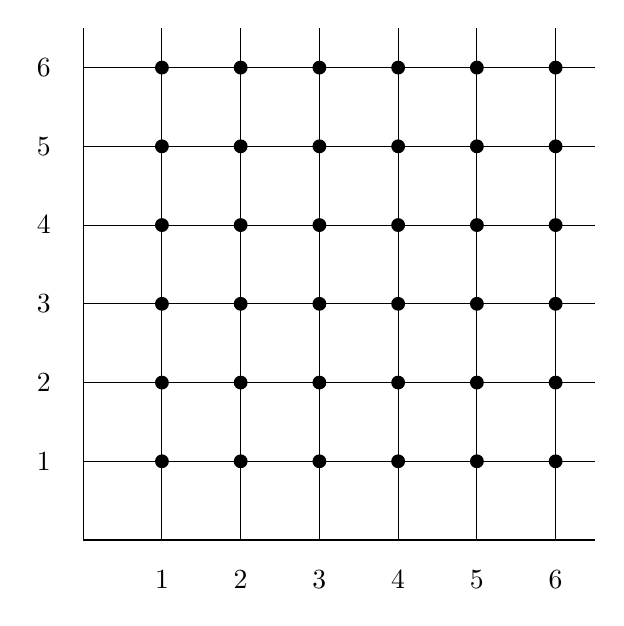
\begin{tikzpicture}
\tikzset{dot/.style={fill=black,circle}}
\draw (0,0) -- (6.5,0);
\draw (0,0) -- (0,6.5);
\foreach\l[count=\y] in {1,2,...,6} {
\draw (0,\y) -- (6.5,\y);
\node at (-0.5,\y){\l}; }
\foreach \x in {1,2,...,6} {
\draw (\x,0) -- (\x,6.5);
\node at (\x,-0.5){\x}; }

\foreach \x in {1,2,...,6} {
\foreach\l[count=\y] in {1,2,...,6} {
\node[circle,fill=black,inner sep=0pt,minimum size=5pt] at (\x, \y){}; }}

\end{tikzpicture}}
\end{center}

From the above possibility diagram, we can see that that the total
number of possible outcomes is $6\times6=36$. Using this diagram
will make it easier for us to find the probability of certain events.

\begin{example}[Possibility Diagram for Dice]

Find the probability of rolling:

\begin{enumerate}[label=(\alph*)]

\item  the same number on both die

\item  a total of 6

\end{enumerate}

\Solution

\begin{center}
\resizebox{6cm}{6cm}{%
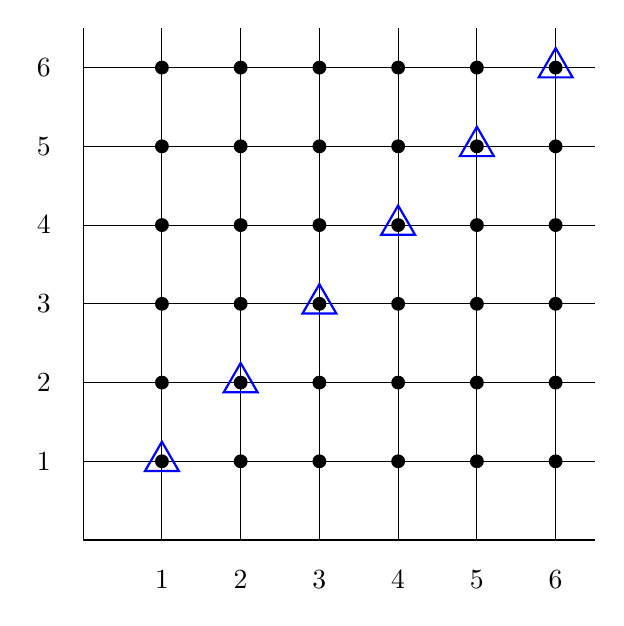
\begin{tikzpicture}
\tikzset{dot/.style={fill=black,circle}}
\draw (0,0) -- (6.5,0);
\draw (0,0) -- (0,6.5);
\foreach\l[count=\y] in {1,2,...,6} {
\draw (0,\y) -- (6.5,\y);
\node at (-0.5,\y){\l}; }
\foreach \x in {1,2,...,6} {
\draw (\x,0) -- (\x,6.5);
\node at (\x,-0.5){\x}; }

\foreach \x in {1,2,...,6} {
\foreach\l[count=\y] in {1,2,...,6} {
\node[circle,fill=black,inner sep=0pt,minimum size=5pt] at (\x, \y){}; }}

\foreach \x in {1,2,...,6} {
\node[thick, draw=blue,regular polygon, regular polygon sides=3,inner sep=2.5pt,] at (\x,\x){};}

\end{tikzpicture}}\hspace{2cm}\resizebox{6cm}{6cm}{%
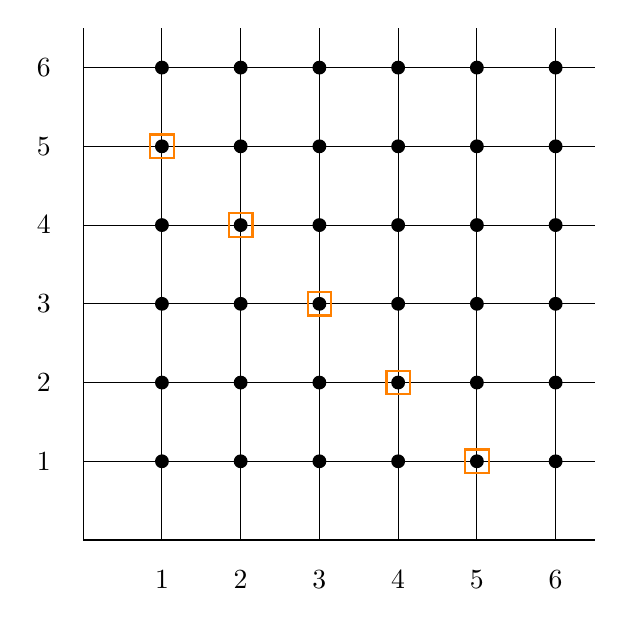
\begin{tikzpicture}
\tikzset{dot/.style={fill=black,circle}}
\draw (0,0) -- (6.5,0);
\draw (0,0) -- (0,6.5);
\foreach\l[count=\y] in {1,2,...,6} {
\draw (0,\y) -- (6.5,\y);
\node at (-0.5,\y){\l}; }
\foreach \x in {1,2,...,6} {
\draw (\x,0) -- (\x,6.5);
\node at (\x,-0.5){\x}; }

\foreach \x in {1,2,...,6} {
\foreach\l[count=\y] in {1,2,...,6} {
\node[circle,fill=black,inner sep=0pt,minimum size=5pt] at (\x, \y){}; }}

\foreach \x in {1,2,...,5} {
\node[thick, draw=orange,regular polygon, regular polygon sides=4,inner sep=3pt,] at (\x,6-\x){};}

\end{tikzpicture}}
\end{center}

\begin{minipage}[t]{.6\textwidth}

\begin{enumerate}[label=(\alph*)]

\item
$
\begin{aligned}[t]
\text{P(same number on both dice)} & =\frac{6}{36} & =\frac{1}{6}
\end{aligned}
$
\end{enumerate}

\end{minipage}
\begin{minipage}[t]{.5\textwidth}

\begin{enumerate}[label=(\alph*),start=2]
\item
$
\begin{aligned}[t]
\text{P(total of 6)} & =\frac{5}{36}
\end{aligned}
$

\end{enumerate}

\end{minipage}

\end{example}


\subsection{Tree Diagrams}

Tree diagrams can be used to illustrate sample spaces, provided that
the alternatives are not too numerous.

Below we see the tree diagram for tossing three fair coins.

\begin{center}
\tikzstyle{level 1}=[level distance=20mm, sibling distance=30mm]
\tikzstyle{level 2}=[level distance=20mm, sibling distance=15mm]
\tikzstyle{level 3}=[level distance=15mm, sibling distance=5mm]
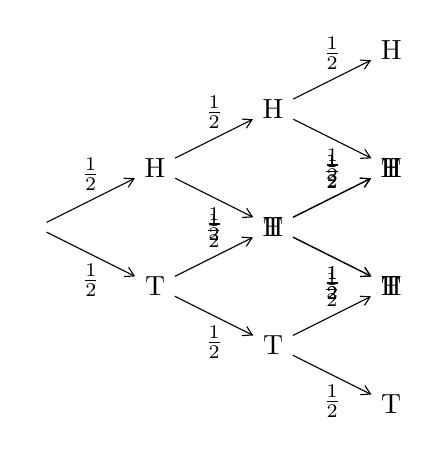
\begin{tikzpicture}[grow=right,->,>=angle 60]
%\begin{scope}[yshift=0]
 \node {}
    child {node {T}
      child {node {T}
        child {node {T}
		edge from parent
		node[below]  {$\frac{1}{2}$}}
        child {node {H}
		edge from parent
		node[above]  {$\frac{1}{2}$}}
            edge from parent
            node[below]  {$\frac{1}{2}$}
		}
      child {node{H}
        child {node {T}
		edge from parent
		node[below]  {$\frac{1}{2}$}}
        child {node {H}
		edge from parent
		node[above]  {$\frac{1}{2}$}}
            edge from parent
            node[above]  {$\frac{1}{2}$}
        }
            edge from parent
            node[below]  {$\frac{1}{2}$}
    }
    child {node {H}
      child {node{T}
        child {node {T}
		edge from parent
		node[below]  {$\frac{1}{2}$}}
        child {node {H}
		edge from parent
		node[above]  {$\frac{1}{2}$}}
       edge from parent
            node[below]  {$\frac{1}{2}$}
        }
      child {node{H}
        child {node {T}
		edge from parent
		node[below]  {$\frac{1}{2}$}}
        child {node {H}
		edge from parent
		node[above]  {$\frac{1}{2}$}}
       edge from parent
            node[above]  {$\frac{1}{2}$}
        }
        edge from parent
            node[above]  {$\frac{1}{2}$}
    };

%\end{scope}
\end{tikzpicture}
\end{center}

From the above tree diagram, we can see that that the total number
of possible outcomes is $2\times2\times2=8$. Tree diagrams are useful for illustrating the sample space when we have \textit{more than two} events occurring in sequence.

\section{Sampling With and Without Replacement}

Sampling is the process of selecting an object from a large group
of objects and inspecting it, noting some feature(s). The object is
then either \textbf{put back} (sampling \textbf{with replacement})
or \textbf{put to one side} (sampling \textbf{without replacement}).

Consider a box containing $3$ red, $2$ blue and $1$ yellow marble.
Suppose we wish to sample two marbles:

\begin{itemize}[leftmargin=4cm]

\item with replacement of the first before the second is drawn

\item without replacement of the first before the second is drawn

\end{itemize}

Examine how the tree diagrams differ:

\textbf{With relplacement \hspace{5.2cm}Without Replacement}

\tikzstyle{level 1}=[level distance=40mm, sibling distance=25mm]
\tikzstyle{level 2}=[level distance=20mm, sibling distance=8mm]
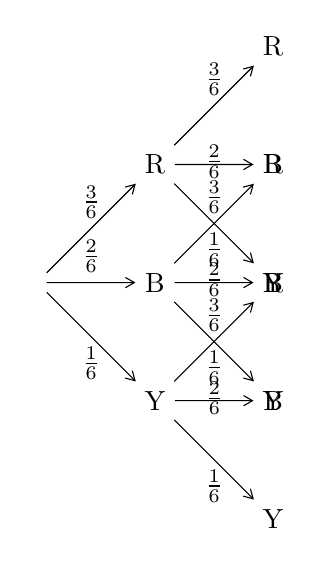
\begin{tikzpicture}[grow=right,->,>=angle 60]
%\begin{scope}[yshift=0]
 \node {}
    child {node {Y}
      child {node {Y}
            edge from parent
            node[below]  {$\frac{1}{6}$}
		}
      child {node{B}
            edge from parent
            node[above,yshift=-0.3cm]  {$\frac{2}{6}$}
        }
      child {node {R}
            edge from parent
            node[above]  {$\frac{3}{6}$}
		}
            edge from parent
            node[below]  {$\frac{1}{6}$}
    }
    child {node {B}
      child {node{Y}
       edge from parent
            node[below]  {$\frac{1}{6}$}
        }
      child {node{B}
       edge from parent
            node[above,yshift=-0.3cm]  {$\frac{2}{6}$}
        }
      child {node {R}
            edge from parent
            node[above]  {$\frac{3}{6}$}
		}
        edge from parent
            node[above]  {$\frac{2}{6}$}
    }
    child {node {R}
      child {node{Y}
       edge from parent
            node[below]  {$\frac{1}{6}$}
        }
      child {node{B}
       edge from parent
            node[above,yshift=-0.3cm]  {$\frac{2}{6}$}
        }
      child {node {R}
            edge from parent
            node[above]  {$\frac{3}{6}$}
		}
        edge from parent
            node[above]  {$\frac{3}{6}$}
};

%\end{scope}
\end{tikzpicture}\hspace{2cm}\tikzstyle{level 1}=[level distance=40mm, sibling distance=25mm]
\tikzstyle{level 2}=[level distance=20mm, sibling distance=8mm]
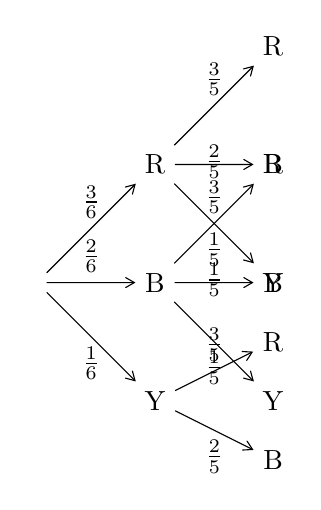
\begin{tikzpicture}[grow=right,->,>=angle 60]
%\begin{scope}[yshift=0]
 \node {}
    child {node {Y}
      child {node{B}
            edge from parent
            node[below]  {$\frac{2}{5}$}
        }
      child {node {R}
            edge from parent
            node[above]  {$\frac{3}{5}$}
		}
            edge from parent
            node[below]  {$\frac{1}{6}$}
    }
    child {node {B}
      child {node{Y}
       edge from parent
            node[below]  {$\frac{1}{5}$}
        }
      child {node{B}
       edge from parent
            node[above,yshift=-0.3cm]  {$\frac{1}{5}$}
        }
      child {node {R}
            edge from parent
            node[above]  {$\frac{3}{5}$}
		}
        edge from parent
            node[above]  {$\frac{2}{6}$}
    }
    child {node {R}
      child {node{Y}
       edge from parent
            node[below]  {$\frac{1}{5}$}
        }
      child {node{B}
       edge from parent
            node[above,yshift=-0.3cm]  {$\frac{2}{5}$}
        }
      child {node {R}
            edge from parent
            node[above]  {$\frac{3}{5}$}
		}
        edge from parent
            node[above]  {$\frac{3}{6}$}
};

%\end{scope}
\end{tikzpicture}

\section{Laws of Probability}

\subsection{Addition Law of Probability}

\centerline{\begin{minipage}{.7\textwidth}
\begin{tcolorbox}[colback=blue!5, colframe=black, boxrule=.4pt, sharpish corners]

The \textbf{addition law of probability} states that for two events
$A$ and $B$,
\[
\text{P}\left(A\cup B\right)=\text{P}\left(A\right)+\text{P}\left(B\right)-\text{P}\left(A\cap B\right)
\]
\end{tcolorbox}
\end{minipage}}

This can be also written as
\[
\text{P}\left(A\textbf{ or }B\right)=\text{P}\left(A\right)+\text{P}\left(B\right)-\text{P}\left(A\textbf{ and }B\right)
\]

Sometimes this law is referred to as the \textbf{Inclusion/Exclusion
Rule}.

\subsection{Mutually Exclusive Events}

\centerline{\begin{minipage}{.65\textwidth}
\begin{tcolorbox}[colback=blue!5, colframe=black, boxrule=.4pt, sharpish corners]

Two events are said to be \textbf{mutually exclusive} if they \textbf{cannot
happen at the same time}.
\end{tcolorbox}
\end{minipage}}

For example, consider the sample space of drawing one card from an
ordinary deck of 52 cards.

\begin{itemize}

\item  $A$ is the event that a spade is drawn,

\item  $B$ is the event that a heart is drawn and

\item  $C$ is the event that an ace is drawn.

\end{itemize}

Events $A$ and $B$ are mutually exclusive because both events cannot
happen at the same time.

Events $A$ and $C$ are not mutually exclusive because we can draw
the Ace of Spades.

Events $B$ and $C$ are also not mutually exclusive.

\medskip

\centerline{\begin{minipage}{.75\textwidth}
\begin{tcolorbox}[colback=blue!5, colframe=black, boxrule=.4pt, sharpish corners]

If $A$ and $B$ are mutually exclusive, then $\text{P}\left(A\cap B\right)=0$.
Thus the addition law for mutually exclusive events becomes
\[
\text{P}\left(A\cup B\right)=\text{P}\left(A\right)+\text{P}\left(B\right)
\]
\end{tcolorbox}
\end{minipage}}

\begin{example}[Conditions for Mutually Exclusive Events and Independent Events]
The events $A$ and $B$ are such that $\text{P}\left(A\right)=0.43$,
$\text{P}\left(B\right)=0.48$, and $\text{P}\left(A\cup B\right)=0.78$.
Show that $A$ and $B$ are neither mutually exclusive nor independent.

\Solution

\begin{align*}
\text{P}\left(A\cup B\right) & =\text{P}\left(A\right)+\text{P}\left(B\right)-\text{P}\left(A\cap B\right)\\
\text{P}\left(A\cap B\right) & =\text{P}\left(A\right)+\text{P}\left(B\right)-\text{P}\left(A\cup B\right)\\
 & =0.43+0.48-0.78\\
 & =0.13\neq0
\end{align*}

Hence, $A$ and $B$ are not mutually exclusive.

\begin{align*}
\text{P}\left(A\right)\times\text{P}\left(B\right) & =0.43\times0.48\\
 & =0.2064\neq0.13=\text{P}\left(A\cap B\right)
\end{align*}

Hence , $A$ and $B$ are not independent.
\end{example}

\newpage

\subsection{Conditional Probability}

Suppose we have two events $A$ and $B$, then

\medskip

\centerline{\begin{minipage}{.65\textwidth}
\begin{tcolorbox}[colback=blue!5, colframe=black, boxrule=.4pt, sharpish corners]

$A\mid B$ is used to represent that ``$A$ occurs \textbf{given}
$B$ has occurred''.
\end{tcolorbox}
\end{minipage}}

\medskip

The \textbf{conditional probability} of event A occurring, given that
event B has occurerd is given by

\medskip

\centerline{\begin{minipage}{.25\textwidth}
\begin{tcolorbox}[colback=blue!5, colframe=black, boxrule=.4pt, sharpish corners]

\[
\text{P}\left(A\mid B\right)=\frac{\text{P}\left(A\cap B\right)}{\text{P}\left(B\right)}
\]
\end{tcolorbox}
\end{minipage}}

\medskip

\begin{example}[Conditional Probability With Dice]

A pair of fair dice are rolled. What is the probability that the sum
of the numbers showing face up is 8, given that both of the numbers
are even?

\Solution

\begin{minipage}{.4\textwidth}

\begin{align*}
\text{P(sum of 8\ensuremath{\mid\text{both are even})}} & =\frac{\text{P(sum of 8 \textbf{and} both are even})}{\text{P(both are even)}}\\
 & =\frac{\frac{3}{36}}{\frac{9}{36}}\\
 & =\frac{1}{3}
\end{align*}

\end{minipage}
\begin{minipage}{.5\textwidth}

\begin{center}
\resizebox{5.5cm}{5.5cm}{%
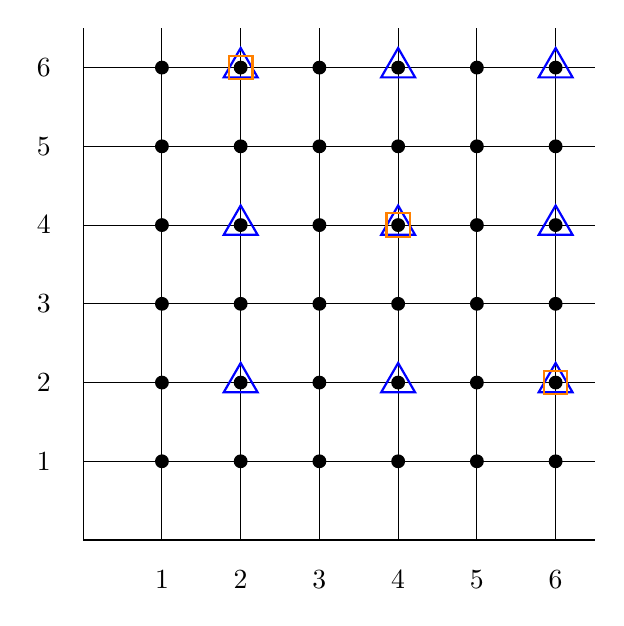
\begin{tikzpicture}
\tikzset{dot/.style={fill=black,circle}}
\draw (0,0) -- (6.5,0);
\draw (0,0) -- (0,6.5);
\foreach\l[count=\y] in {1,2,...,6} {
\draw (0,\y) -- (6.5,\y);
\node at (-0.5,\y){\l}; }
\foreach \x in {1,2,...,6} {
\draw (\x,0) -- (\x,6.5);
\node at (\x,-0.5){\x}; }

\foreach \x in {1,2,...,6} {
\foreach\l[count=\y] in {1,2,...,6} {
\node[circle,fill=black,inner sep=0pt,minimum size=5pt] at (\x, \y){}; }}

\foreach \x in {2,4,6}
\foreach \y in {2,4,6}
{
\node[thick, draw=blue,regular polygon, regular polygon sides=3,inner sep=2.5pt,] at (\x,\y){};}

\node[thick, draw=orange,regular polygon, regular polygon sides=4,inner sep=3pt,] at (2,6){};
\node[thick, draw=orange,regular polygon, regular polygon sides=4,inner sep=3pt,] at (4,4){};
\node[thick, draw=orange,regular polygon, regular polygon sides=4,inner sep=3pt,] at (6,2){};


\end{tikzpicture}}
\end{center}

\end{minipage}

\end{example}

It follows that

\[
\text{P}\left(A\cap B\right)=\text{P}\left(B\right)\times\text{P}\left(A\mid B\right)=\text{P}\left(A\right)\times\text{P}\left(B\mid A\right)
\]

$A$ and $B$ are \textbf{independent events} if the occurrence (or non-occurrence)
of one event does not affect the occurrence of the other,

\[
\text{i.e.}\quad\text{P}\left(A\mid B\right)=\text{P\ensuremath{\left(A\right)}}\quad\text{and}\quad\text{P}\left(B\mid A\right)=\text{P\ensuremath{\left(B\right)}}
\]

So,

\medskip

\centerline{\begin{minipage}{.6\textwidth}
\begin{tcolorbox}[colback=blue!5, colframe=black, boxrule=.4pt, sharpish corners]

$A$ and $B$ are \textbf{independent events} \textbf{$\Leftrightarrow$}
$\text{P}\left(A\cap B\right)=\text{P}\left(A\right)\times\text{P}\left(B\right)$
\end{tcolorbox}
\end{minipage}}

\newpage

\begin{example}[Using Tree Diagrams]

In an archery competition, Bill is allowed up to three attempts to
hit the target. If he succeeds on any attempt, he does not make any
more attempts. The probability that he will hit the target on the
first attempt is $0.6$. If he misses, the probability that he will
hit the target on his second attempt is $0.7$. If he misses the second
attempt, the probability that he will hit the target on his third
attempt is $0.8$.

\begin{enumerate}[label=(\alph*)]

\item Draw a fully labelled tree diagram.

\item Find the probability that Bill hits the target.

\item Given that Bill hits the target, find the probability that
he made at least two attempts.

\end{enumerate}

\Solution

\begin{enumerate}[label=(\alph*)]

\item \leavevmode\vadjust{\vspace{-\baselineskip}}\newline \tikzstyle{level 1}=[level distance=30mm, sibling distance=20mm]
\tikzstyle{level 2}=[level distance=30mm, sibling distance=20mm]
\tikzstyle{level 3}=[level distance=30mm, sibling distance=20mm]
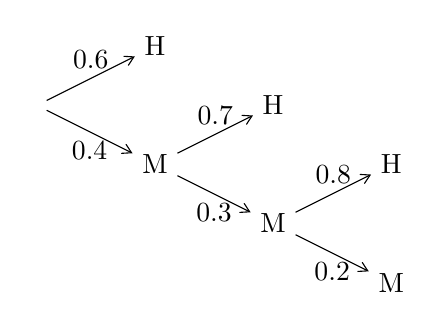
\begin{tikzpicture}[grow=right,->,>=angle 60]
%\begin{scope}[yshift=0]
 \node {}
    child {node {M}
      child {node{M}
		child{node{M}
				edge from parent
				node[below] {$0.2$}}
		child{node{H}
				edge from parent
				node[above] {$0.8$}}
            edge from parent
            node[below]  {$0.3$}
        }
      child {node {H}
            edge from parent
            node[above]  {$0.7$}
		}
            edge from parent
            node[below]  {$0.4$}
    }
    child {node {H}
        edge from parent
            node[above]  {$0.6$}
};

%\end{scope}
\end{tikzpicture}

H: Hit, M: Miss

\item
$
\begin{aligned}[t]
\text{P}\left(\text{Bill hits target}\right) & =0.6+0.4\times0.7+0.4\times0.3\times0.8\\
 & =0.976
\end{aligned}
$

\item
$
\begin{aligned}[t]
\text{P}\left(\text{at least 2 attempts \ensuremath{\mid} hits target}\right) & =\frac{\text{P}\left(\text{at least 2 attempts and hits target}\right)}{\text{P}\left(\text{hits target}\right)}\\
 & =\frac{0.976-0.6}{0.976}\\
 & =\frac{47}{122}
\end{aligned}
$

\end{enumerate}
\end{example}

\section{Probabilities Using Permutations and Combinations}

Permutations and combinations can sometimes be used to find probabilities
of various events particularly when large sample sizes occur. It
is useful to remember that
\[
\text{P}\left(A\right)=\frac{\text{Total number of ways for event \ensuremath{A} to occur}}{\text{Total number of ways to perform the experiment}}
\]

For example, if we select at random a team of 4 boys and 3 girls from
a squad of 8 boys and 7 girls, the total number of unrestricted possibilities
is $^{15}C_{7}$. The number of combinations with the restriction
of ``4 boys and 3 girls'' is $^{8}C_{4}\times{}^{7}C_{3}$.
\[
\therefore\text{P(4 boys and 3 girls)}=\frac{^{8}C_{4}\times{}^{7}C_{3}}{^{15}C_{7}}
\]

The biggest hurdle in probability problems involving permutations
or combinations seems to be in sorting out which to use. Remember

\begin{itemize}[leftmargin=2cm]

\item \textbf{permutations} involve \textbf{arrangements} of letters/people/things,
whereas

\item \textbf{combinations} involve \textbf{selections} such as
committees/teams/delegations.

\end{itemize}

\begin{example}[Finding Probabilities Using PnC]

5 girls and 7 boys are to be seated in a row. What is the probability
that

\begin{enumerate}[label=(\alph*)]

\item not all the girls are seated next to one another?

\item all the girls are not seated next to one another?

\item 3 particular boys are to be seated together?

\item either all the girls are not seated next to one another or
the 3 particular boys are to be seated together or both?

\end{enumerate}

\Solution

\begin{enumerate}[label=(\alph*)]

\item  Group the 5 girls as 1 unit.

\begin{align*}
\text{P}\left(\text{not all the girls are seated next to one another}\right) & =1-\text{P}\left(\text{all girls are seated next to each other}\right)\\
 & =1-\frac{8!\times5!}{12!}\\
 & =\frac{98}{99}
\end{align*}

\item  \_ B \_ B \_ B \_ B \_ B \_ B \_ B \_
\begin{align*}
\text{P}\left(\text{all the girls are not seated next to one another}\right) & =\frac{7!\times{}^{8}P_{5}}{12!}\\
 & =\frac{7}{99}
\end{align*}

\item Group the 3 boys as 1 unit.
\begin{align*}
\text{P}\left(\text{3 particular boys are seated together}\right) & =\frac{10!\times3!}{12!}\\
 & =\frac{1}{22}
\end{align*}

\item  Let $A$ and $B$ denote the events that all the girls are
not seated next to one another and that the 3 particular boys are
seated together respectively. Then

\begin{align*}
\text{P}\left(A\cap B\right) & =\frac{5!\times3!\times{}^{6}P_{5}}{12!}\\
 & =\frac{1}{924}
\end{align*}

Hence,
\begin{align*}
\text{P}\left(A\cup B\right) & =\text{P}\left(A\right)+\text{P}\left(B\right)-\text{P}\left(A\cap B\right)\\
 & =\frac{7}{99}+\frac{1}{22}-\frac{1}{924}\\
 & =\frac{29}{252}
\end{align*}

\end{enumerate}
\end{example}

\newpage{}

\section{De Meres Problem}

Gamblers in 1654 France used to bet on the event of getting at least
one six in four rolls of a dice. As a more trying variation, two die
were rolled 24 times with a bet on having at least one double six.
De Méré's problem is as follows:

\begin{example}[De Meres Problem]

Is it more likely to get at least one double six in 24 rolls
of a pair of dice or to get at least one six in four rolls
of a single die?

\Solution

\begin{align*}
\text{P}\left(\text{at least one six in four rolls}\right) & =1-\text{P}\left(\text{no six in four rolls}\right)\\
 & =1-\left(\frac{5}{6}\right)^{4}\\
 & =0.518\text{ (3 s.f.)}
\end{align*}

\begin{align*}
\text{P}\left(\text{at least one double six in 24 rolls}\right) & =1-\text{P}\left(\text{no double six in 24 rolls}\right)\\
 & =1-\left(\frac{35}{36}\right)^{24}\\
 & =0.491\text{ (3 s.f.)}
\end{align*}

Thus is it more likely that we roll at least one six in four rolls.

\end{example}

\section{Newton-Pepys Problem}

\begin{example}[Newton-Pepys Problem]

In 1693 Samuel Pepys and Isaac Newton corresponded over a problem
posed by Pepys in relation to a wager he planned to make. Pepys asked
which was more likely,

\begin{enumerate}[label=\Alph*:]

\item At least one six when six dice are rolled,

\item At least two sixes when 12 dice are rolled, or

\item At least three sixes when 18 dice are rolled.

\end{enumerate}

Pepys initially thought that outcome C had the highest probability.
Check to see if he was right or wrong by finding each of the corresponding
probabilities.

\Solution

$
\begin{aligned}[t]
\text{P}\left(\text{at least one six in six rolls}\right) & =1-\text{P}\left(\text{no six in six rolls}\right)\\
 & =1-\left(\frac{5}{6}\right)^{6}\\
 & =0.665\text{ (3 s.f.)}
\end{aligned}
$

$
\begin{aligned}[t]
\text{P}\left(\text{at least two sixes in 12 rolls}\right) & =1-\text{P}\left(\text{less than two sixes in 12 rolls}\right)\\
 & =1-\left[\text{P}\left(\text{no six in 12 rolls}\right)+\text{P}\left(\text{one six in 12 rolls}\right)\right]\\
 & =1-\left[\left(\frac{5}{6}\right)^{12}+\left(\frac{1}{6}\right)\left(\frac{5}{6}\right)^{11}\times{}^{12}C_{1}\right]\\
 & =0.619\text{ (3 s.f.)}
\end{aligned}
$

$
\begin{aligned}[t]
\text{P}\left(\text{at least three sixes in 18 rolls}\right) & =1-\text{P}\left(\text{less than three sixes in 18 rolls}\right)\\
 & =1-\left[\text{P}\left(\text{no six in 18 rolls}\right)+\text{P}\left(\text{one six in 18 rolls}\right)+\text{P}\left(\text{two sixes in 18 rolls}\right)\right]\\
 & =1-\left[\left(\frac{5}{6}\right)^{18}+\left(\frac{1}{6}\right)\left(\frac{5}{6}\right)^{17}\times{}^{18}C_{1}+\left(\frac{1}{6}\right)^{2}\times\left(\frac{5}{6}\right)^{16}\times{}^{18}C_{2}\right]\\
 & =0.597\text{ (3 s.f.)}
\end{aligned}
$

\end{example}

\section{The St. Petersberg Paradox}

A casino offers a game of chance for a single player in which a fair
coin is tossed at each stage. The initial stake begins at 2 dollars
and is doubled every time heads appears. The first time tails appears,
the game ends and the player wins whatever is in the pot. Thus the
player wins 2 dollars if tails appears on the first toss, 4 dollars
if heads appears on the first toss and tails on the second, 8 dollars
if heads appears on the first two tosses and tails on the third, and
so on.

Mathematically, the player wins $2^{k}$ dollars, where $k$ is the
number of consecutive head tosses. What would be a fair price to pay
the casino for entering the game?

To answer this, one needs to consider what would be the expected payout
at each stage: with probability ${\displaystyle \frac{1}{2}}$ the
player wins 2 dollars; with probability ${\displaystyle \frac{1}{4}}$
the player wins 4 dollars; with probability ${\displaystyle \frac{1}{8}}$
the player wins 8 dollars, and so on. Assuming the game can continue
as long as the coin toss results in heads and, in particular, that
the casino has unlimited resources, the expected value is thus

\begin{align*}
\text{E}\left(X\right) & =\frac{1}{2}\times2+\frac{1}{4}\times4+\frac{1}{8}\times8+\frac{1}{16}\times16+\ldots\\
 & =1+1+1+1+\ldots\\
 & =\infty
\end{align*}

Considering nothing but the expected value of the net change in one's
monetary wealth, one should therefore play the game at any price if
offered the opportunity. In a strict logical sense, the St. Petersburg
paradox is not a paradox because no formal contradiction is derived.
However, to claim that a rational agent should pay millions, or even
billions, for playing this game seems absurd. Few of us would be willing
to pay even $\$20$ to enter such a game.

\newpage{}

\section{The Monty Hall Problem}

The next example is called the Monty Hall problem, named for the first
host of the game show \textquotedblleft Let\textquoteright s Make
A Deal.\textquotedblright{} When it was originally publicized in a
newspaper column and on a radio show, it created tremendous controversy.
Many highly educated people, even some with Ph.D.\textquoteright s,
submitted incorrect solutions or argued vociferously against the correct
solution. Before you read the answer, think about what your own response
to the situation would be.

\begin{example}[The Monty Hall Problem]

There are three doors on the set for a game show. Let\textquoteright s
call them $A$, $B$, and $C$. Behind one of the doors, there is
a car. If you pick the correct door, you win the car. You pick door
$A$. The host of the show then opens one of the other doors and reveals
that there is no car behind it. Keeping the remaining two doors closed,
he asks you whether you want to switch your choice to the other closed
door or stay with your original choice of door $A$. What should you
do if you want to maximize your chance of winning the car: stay with
door $A$ or switch---or would the likelihood of winning be the same
either way?

\Solution

\begin{center}
\setlength{\extrarowheight}{2pt}%
\begin{tabular}{|>{\centering}p{4cm}|>{\centering}p{4cm}|>{\centering}p{4cm}|}
\hline
Case 1 & Case 2 & Case 3\tabularnewline
\hline
$B$\hspace{1.3cm}$C$ & $B$\hspace{1.3cm}$C$ & $B$\hspace{1.3cm}$C$\tabularnewline
\includegraphics[width=3cm]{\string"lib/Graphics/MontyHallDoor\string".png} & \includegraphics[width=3cm]{\string"lib/Graphics/MontyHallDoor2\string".png} & \includegraphics[width=3cm]{\string"lib/Graphics/MontyHallDoor3\string".png}\tabularnewline
\hline
\end{tabular}
\par\end{center}

At the point just before the host opens one of the closed doors, there
is no information about the location of the prize. Thus there are
three equally likely possibilities for what lies behind the doors:
(Case 1) the prize is behind $A$; (Case 2) the prize is behind $B$;
or (Case 3) the prize is behind $C$. Since there is no prize behind
the door the host opens, in Case 1 the host could open either door
and you would win by staying with your original choice: door $A$.
In Case 2 the host must open door $C$, and so you would win by switching
to door $B$. In Case 3 the host must open door $B$, and so you would
win by switching to door $C$. Thus, in two of the three equally likely
cases, you would win by switching from $A$ to the other closed door.
In only one of the three equally likely cases would you win by staying
with your original choice. Therefore, \textbf{you should switch}.
\end{example}


\newpage

\section*{Probability Summary}
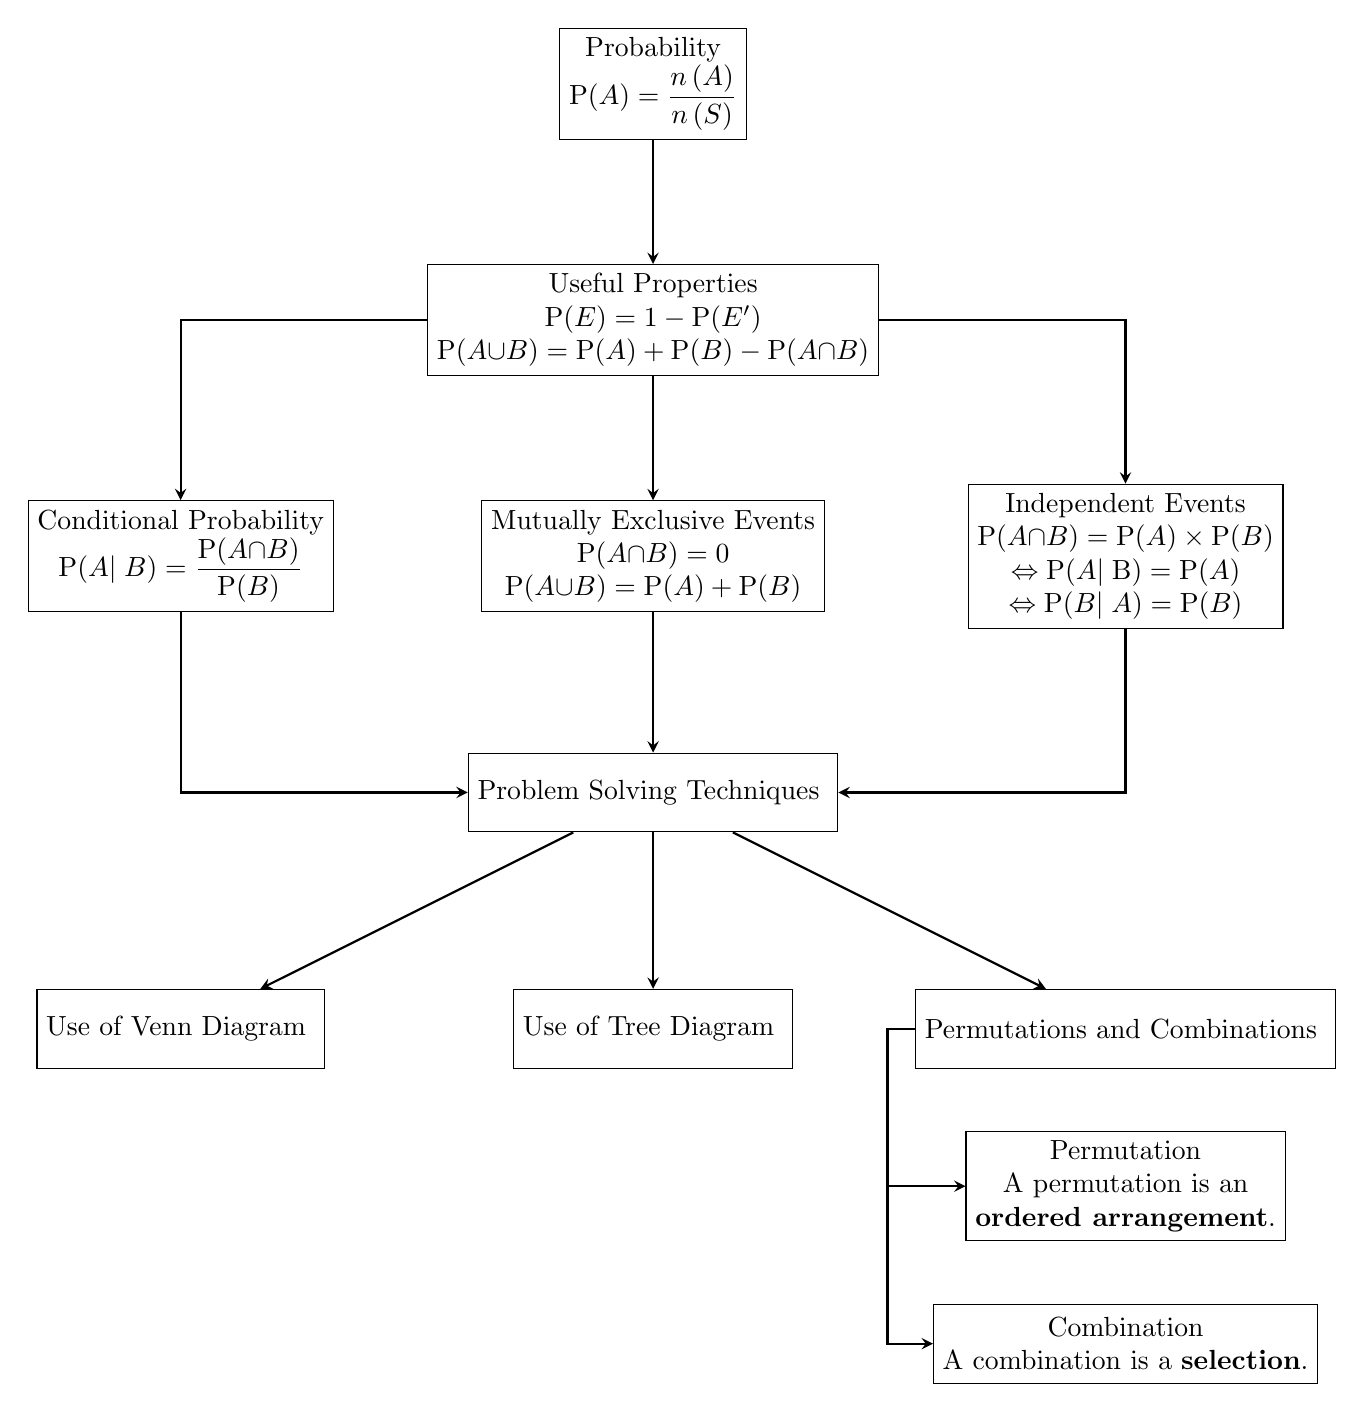
\begin{tikzpicture}[every text node part/.style={align=center}]
\node (Probability)[Box]{Probability \\
${\displaystyle \text{P($A$)}=\frac{n\left(A\right)}{n\left(S\right)}}$
};
\node (Useful Properties)[Box, below of = Probability, yshift=-2cm]{Useful Properties \\
$\text{P($E$)}=1-\text{P($E'$)}$ \\
$\text{P($A$\ensuremath{\cup}$B$})=\text{P($A$)}+\text{P($B$)}-\text{P($A$\ensuremath{\cap}$B$})$
};
\node (Mutually Exclusive)[Box, below of = Useful Properties, yshift=-2cm]{Mutually Exclusive Events \\
$\text{P($A$\ensuremath{\cap}$B$})=0$ \\
$\text{P($A$\ensuremath{\cup}$B$})=\text{P($A$)}+\text{P($B$)}$
};
\node (Independent Events)[Box, right of = Mutually Exclusive, xshift=5cm]{Independent Events \\
$\text{P($A$\ensuremath{\cap}$B$})=\text{P($A$)}\times\text{P($B$)}$\\
$\Leftrightarrow\text{P($A$\ensuremath{\mid\text{B})}}=\text{P\ensuremath{\left(\text{$A$}\right)}}$ \\
$\Leftrightarrow\text{P($B$\ensuremath{\mid\text{$A$})}}=\text{P\ensuremath{\left(\text{$B$}\right)}}$
};
\node (Conditional Probability)[Box, left of = Mutually Exclusive, xshift=-5cm]{Conditional Probability \\
${\displaystyle \text{P($A$\ensuremath{\mid\text{$B$})=\frac{\text{P($A$\ensuremath{\cap}$B$})}{\text{P($B$)}}}}}$
};
\node (Problem Solving)[Box, below of = Mutually Exclusive, yshift=-2cm]{Problem Solving Techniques
};
\node (Tree Diagram)[Box, below of = Problem Solving, yshift=-2cm]{Use of Tree Diagram
};
\node (Venn Diagram)[Box, left of = Tree Diagram, xshift=-5cm]{
Use of Venn Diagram
};
\node (Permutations and Combinations)[Box, right of = Tree Diagram, xshift=5cm]{Permutations and Combinations
};

\node (Permutations)[Box, below of = Permutations and Combinations,yshift=-1cm]{Permutation \\
A permutation is an \\
\textbf{ordered arrangement}.
};
\node (Combinations)[Box, below of = Permutations, yshift=-1cm]{Combination \\
A combination is a \textbf{selection}.
};

\draw[arrow](Probability)--(Useful Properties);
\draw[arrow](Useful Properties)--(Mutually Exclusive);
\draw[arrow](Useful Properties)-|(Conditional Probability);
\draw[arrow](Useful Properties)-|(Independent Events);
\draw[arrow](Mutually Exclusive)--(Problem Solving);
\draw[arrow](Conditional Probability)|-(Problem Solving);
\draw[arrow](Independent Events)|-(Problem Solving);
\draw[arrow](Problem Solving)--(Tree Diagram);
\draw[arrow](Problem Solving)--(Venn Diagram);
\draw[arrow](Problem Solving)--(Permutations and Combinations);
\draw[arrow](Permutations and Combinations.west)--++(-10pt,0pt) |- (Permutations.west);
\draw[arrow](Permutations and Combinations.west)--++(-10pt,0pt) |- (Combinations.west);


\end{tikzpicture}

\chapter{Discrete Random Variables}
\section{Discrete Random Variables}
\centerline{\begin{minipage}{.75\textwidth}
\begin{tcolorbox}[colback=blue!5, colframe=black, boxrule=.4pt, sharpish corners]

A \textbf{random variable} is a numerical quantity that is generated
by a random experiment, we denote random variables by capital letters
such as $X$.
\end{tcolorbox}
\end{minipage}}

\medskip

A random variable can be \textbf{discrete} or \textbf{continuous}.

\medskip

\centerline{\begin{minipage}{.88\textwidth}
\begin{tcolorbox}[colback=blue!5, colframe=black, boxrule=.4pt, sharpish corners]

A random variable $X$ is called \textbf{discrete} if it has a \textbf{countable}
number of possible values.
\end{tcolorbox}
\end{minipage}}

\medskip

For example, $X$ could be:

\begin{itemize}

\item  the number of rotten apples in a basket of fuits,

\item  the number of males in a group of $5$ students,

\item  the number of new bicycles sold each year by a bicycle store.

\end{itemize}

\medskip

\medskip

\centerline{\begin{minipage}{.75\textwidth}
\begin{tcolorbox}[colback=blue!5, colframe=black, boxrule=.4pt, sharpish corners]

A random variable $X$ is called \textbf{continuous} if it takes on
a \textbf{range} of values.
\end{tcolorbox}
\end{minipage}}

\medskip

For example, $X$ could be:

\begin{itemize}

\item  the height of a randomly selected student,

\item  the weight of a randomly selected bag of sugar,

\item  the time taken for a randomly selected student to complete
a $2.4\,\text{km}$ run.

\end{itemize}

Consider the experiment of tossing a fair coin $3$ times and observing
the outcome.

The sample space may be represented by

\[
\left\{ HHH,HHT,HTH,HTT,THH,THT,TTH,TTT\right\}
\]

\medskip

Let $X$ denote the number of heads obtained when tossing a fair coin
$3$ times.
\begin{itemize}
\item The possible values (variable) $X$ can take are $0$, $1$, $2$,
$3$ (discrete). The value it assumes is subject to chance (random).
Thus $X$ is a discrete random variable.
\item $\text{P}\left(X=x\right)$ refers to the probability of the discrete
random variable $X$ assuming a specific value $x$.
\item E.g. $\text{P}\left(X=2\right)$ refers to the probabiltiy of obtaining
two heads in $3$ tosses. In this case, ${\displaystyle \text{P}\left(X=2\right)=\frac{3}{8}}$
\end{itemize}
\newpage{}

\section{Probability Distribution}

The \textbf{probability distribution} is a table that lists down each
probability $\text{P}\left(X=x\right)$ for all possible values of
$x$.

\setlength{\extrarowheight}{2pt}
\begin{center}
\begin{tabular}{|>{\centering}m{2cm}|>{\centering}m{2cm}|>{\centering}m{2cm}|>{\centering}m{2cm}|}
\hline
$x$ &  &  & \tabularnewline
\hline
$\text{P}\left(X=x\right)$ &  &  & \tabularnewline
\hline
\end{tabular}
\par\end{center}

For the experiment of tossing a fair coin 3 times where $X$ is the
number of heads obtained, the probability distribution of $X$ is
as follows

\setlength{\extrarowheight}{2pt}
\begin{center}
\begin{tabular}{|>{\centering}m{2cm}|>{\centering}m{2cm}|>{\centering}m{2cm}|>{\centering}m{2cm}|>{\centering}m{2cm}|}
\hline
$x$ & 0 & 1 & 2 & 3\tabularnewline
\hline
\medskip

$\text{P}\left(X=x\right)$

\smallskip & \medskip

${\displaystyle \frac{1}{8}}$

\smallskip & \medskip

${\displaystyle \frac{3}{8}}$

\smallskip & \medskip

${\displaystyle \frac{3}{8}}$

\smallskip & \medskip

${\displaystyle \frac{1}{8}}$

\smallskip\tabularnewline
\hline
\end{tabular}
\par\end{center}

For a discrete random variable $X$, the sum of probabilities is $\textbf{1}$:
\[
\sum_{\text{all}\,x}\text{P}\left(X=x\right)=1
\]

\begin{example}[Probability Distribution For a Spinner]

\begin{minipage}[t]{.6\textwidth}

Let $X$ be the result when the spinner alongside is spun.

\begin{enumerate}[label=(\alph*)]

\item  Display the probability distribution of $X$ in a table.

\item  Find $\text{P}\left(X\leq3\right)$.

\item  Find $\text{P}\left(1<X<4\right)$.

\end{enumerate}

\end{minipage}
\begin{minipage}[t]{.38\textwidth}
\begin{center}
\includegraphics[width=3cm,valign=t]{\string"lib/Graphics/SpinnerDRV\string".png}
\par\end{center}

\end{minipage}

\Solution

\begin{enumerate}[label=(\alph*)]

\item

\setlength{\extrarowheight}{2pt}%
\begin{tabular}[t]{|>{\centering}m{2cm}|>{\centering}m{2cm}|>{\centering}m{2cm}|>{\centering}m{2cm}|>{\centering}m{2cm}|}
\hline
$x$ & 1 & 2 & 3 & 4\tabularnewline
\hline
\medskip

$\text{P}\left(X=x\right)$

\smallskip & \medskip

${\displaystyle \frac{3}{8}}$

\smallskip & \medskip

${\displaystyle \frac{1}{4}}$

\smallskip & \medskip

${\displaystyle \frac{1}{8}}$

\smallskip & \medskip

${\displaystyle \frac{1}{4}}$

\smallskip\tabularnewline
\hline
\end{tabular}

\item
$
\begin{aligned}[t]
\text{P}\left(X\leq3\right) & =1-\text{P}\left(X=4\right)\\
 & =1-\frac{1}{4}\\
 & =\frac{3}{4}
\end{aligned}
$

\item
$
\begin{aligned}[t]
\text{P}\left(1<X<4\right) & =\text{P}\left(X=2\right)+\text{P}\left(X=3\right)\\
 & =\frac{1}{4}+\frac{1}{8}\\
 & =\frac{3}{8}
\end{aligned}
$

\end{enumerate}

\end{example}

\newpage

\begin{example}[Probability Distribution Function]

The probabilities that a discrete random variable $X$ takes are given
by $\text{P}\left(X=x\right)=cx^{2}$ where $x\in\left\{ 1,2,3,4\right\} $.
Given that $c$ is a constant, find the value of $c$. Hence display
the probability distribution of $X$.

\Solution

\begin{align*}
\text{P}\left(X=1\right) & =c\left(1\right)^{2}\\
\text{P}\left(X=2\right) & =c\left(2\right)^{2}\\
\text{P}\left(X=3\right) & =c\left(3\right)^{2}\\
\text{P}\left(X=4\right) & =c\left(4\right)^{2}
\end{align*}

Since the sum of probabilities is equal to 1,

\begin{align*}
c\left(1\right)^{2}+c\left(2\right)^{2}+c\left(3\right)^{2}+c\left(4\right)^{2} & =1\\
30c & =1\\
c & =\frac{1}{30}
\end{align*}

\begin{center}
\setlength{\extrarowheight}{2pt}%
\begin{tabular}[t]{|>{\centering}m{2cm}|>{\centering}m{2cm}|>{\centering}m{2cm}|>{\centering}m{2cm}|>{\centering}m{2cm}|}
\hline
$x$ & 1 & 2 & 3 & 4\tabularnewline
\hline
\medskip

$\text{P}\left(X=x\right)$

\smallskip & \medskip

${\displaystyle \frac{1}{30}}$

\smallskip & \medskip

${\displaystyle \frac{2}{15}}$

\smallskip & \medskip

${\displaystyle \frac{3}{10}}$

\smallskip & \medskip

${\displaystyle \frac{8}{15}}$

\smallskip\tabularnewline
\hline
\end{tabular}
\par\end{center}

\end{example}

\newpage

\section{Expected Value of a Random Variable}

The \textbf{expected value} or \textbf{mean} of a discrete random
variable of $X$, $E\left(X\right)$, is given by:
\[
\text{E}\left(X\right)=\sum_{\text{all}\,x}x\text{P}\left(X=x\right)
\]

$\text{E}\left(X\right)$ is also denoted by the symbol $\mu$.

\begin{example}[Finding Expected Value Using a Probability Distribution]

Find $\text{E}\left(X\right)$ for the probability distribution in \textsf{Example 2.2}.

\Solution

\begin{center}
\setlength{\extrarowheight}{2pt}%
\begin{tabular}[t]{|>{\centering}m{2cm}|>{\centering}m{2cm}|>{\centering}m{2cm}|>{\centering}m{2cm}|>{\centering}m{2cm}|}
\hline
$x$ & 1 & 2 & 3 & 4\tabularnewline
\hline
\medskip

$\text{P}\left(X=x\right)$

\smallskip & \medskip

${\displaystyle \frac{1}{30}}$

\smallskip & \medskip

${\displaystyle \frac{2}{15}}$

\smallskip & \medskip

${\displaystyle \frac{3}{10}}$

\smallskip & \medskip

${\displaystyle \frac{8}{15}}$

\smallskip\tabularnewline
\hline
\end{tabular}
\par\end{center}

\begin{align*}
\text{E}\left(X\right) & =1\times\frac{1}{30}+2\times\frac{2}{15}+3\times\frac{3}{10}+4\times\frac{8}{15}\\
 & =\frac{10}{3}
\end{align*}

\end{example}

\begin{example}[Finding Unknowns in a Probability Distribution]

Given that $\text{E}\left(X\right)=2.5$, find $a$ and $b$.
\begin{center}
\setlength{\extrarowheight}{2pt}%
\begin{tabular}[t]{|>{\centering}m{2cm}|>{\centering}m{1.5cm}|>{\centering}m{1.5cm}|>{\centering}m{1.5cm}|>{\centering}m{1.5cm}|}
\hline
$x$ & 1 & 2 & 3 & 4\tabularnewline
\hline
$\text{P}\left(X=x\right)$ & $0.3$ & $a$ & $b$ & $0.2$\tabularnewline
\hline
\end{tabular}
\par\end{center}

\Solution

Since the sum of probabilities is equal to $1$,
\begin{align*}
0.3+a+b+0.2 & =1\\
a+b & =0.5\tag{1}
\end{align*}

Since $\text{E}\left(X\right)=2.5$,
\begin{align*}
1\times0.3+2\times a+3\times b+4\times0.2 & =2.5\\
2a+3b & =1.4\tag{2}
\end{align*}

Solving (1) and (2), $a=0.1$ and $b=0.4$.
\end{example}

\newpage

\begin{example}[Game of Chance]

In a game of chance, a player spins a square spinner labelled $1,2,3,4$.
The player wins the amount of money according to the table below.
\begin{center}
\setlength{\extrarowheight}{2pt}%
\begin{tabular}[t]{|>{\centering}m{2cm}|>{\centering}m{1.5cm}|>{\centering}m{1.5cm}|>{\centering}m{1.5cm}|>{\centering}m{1.5cm}|}
\hline
Number & 1 & 2 & 3 & 4\tabularnewline
\hline
Winnings & $\$1$ & $\$2$ & $\$5$ & $\$8$\tabularnewline
\hline
\end{tabular}
\par\end{center}

\begin{enumerate}[label=(\alph*)]

\item  Find the expected payout for one spin of the spinner.

\item  Find the expected gain for one spin if it costs $\$5$ to
play each game.

\item  Discuss whether you would reccomend playing this game.

\end{enumerate}

\Solution

\begin{enumerate}[label=(\alph*)]

\item  Let $X$ denote the payout from one spin.

Each outcome is equally likely, so the probability of each outcome
is ${\displaystyle \frac{1}{4}}$.

\begin{align*}
\text{E}\left(X\right) & =\frac{1}{4}\times1+\frac{1}{4}\times2+\frac{1}{4}\times5+\frac{1}{4}\times8\\
 & =\$4
\end{align*}

\item  Let $Y$ denote the gain of the player from each game.

Since it costs $\$5$ to play the game, the expected gain is
\begin{align*}
\text{E}\left(Y\right) & =\text{E}\left(X\right)-5\\
 & =4-5\\
 & =-\$1
\end{align*}

\item  Since $\text{E}\left(Y\right)=-\$1$, we expect the player
to lose $\$1$ on average for each spin. We would not recommend a
person play the game (unless the fun of each spin is worth more than
$\$1$ to them).

\end{enumerate}
\end{example}


\begin{example}[Expectation of $X$]

Find $c$ and $\text{E}\left(X\right)$.
\begin{center}
\setlength{\extrarowheight}{2pt}%
\begin{tabular}[t]{|>{\centering}m{2cm}|>{\centering}m{1.5cm}|>{\centering}m{1.5cm}|>{\centering}m{1.5cm}|>{\centering}m{1.5cm}|>{\centering}m{1.5cm}|}
\hline
$x$ & $-2$ & $-1$ & $0$ & $1$ & $2$\tabularnewline
\hline
$\text{P}\left(X=x\right)$ & $0.3$ & $c$ & $0.15$ & $0.4$ & $0.05$\tabularnewline
\hline
\end{tabular}
\par\end{center}

\Solution

Since the sum of probabilities is equal to $1$,

\begin{align*}
0.3+c+0.15+0.4+0.05 & =1\\
c & =0.1
\end{align*}

\begin{align*}
\text{E}\left(X\right) & =\left(-2\times0.3\right)+\left(-1\times0.1\right)+\left(0\times0.15\right)+\left(1\times0.4\right)+\left(2\times0.05\right)\\
 & =-0.2
\end{align*}

\end{example}

\begin{tcolorbox}[colback=blue!5, colframe=black, boxrule=.4pt, sharpish corners]

Let $X$ be a discrete random variable which takes values from a set
$S$.

If $g\left(X\right)$ is a function of $X$, then $g\left(X\right)$
is also a discrete random variable and
\[
\text{E}\left[g\left(x\right)\right]=\sum_{\text{all}\,x}g\left(x\right)\text{P}\left(X=x\right)
\]
where the summation is over all elements $x$ in $S$.

For any random variables $X$ and $Y$,

\begin{enumerate}[label=(\alph*)]

\item  $\text{E}\left(a\right)=a$

\item  $\text{E}\left(aX\right)=a\text{E}\left(X\right)$

\item  $\text{E}\left(aX\pm b\right)=a\text{E}\left(X\right)\pm b$

\item  $\text{E}\left(aX\pm bY\right)=a\text{E}\left(X\right)\pm b\text{E}\left(Y\right)$

\end{enumerate}

where $a$ and $b$ are constants.

\end{tcolorbox}

\medskip

\begin{example}[Expectation of $g(X)$]

With $X$ as defined in \textsf{Example 2.6}, find $\text{E}\left(X^{2}\right)$
and $\text{E}\left(\left|X+1\right|\right)$.

Hence, find the value of $\text{E}\left(3X^{2}-2\left|X+1\right|\right)$.

\Solution

\begin{center}
\setlength{\extrarowheight}{2pt}%
\begin{tabular}[t]{|>{\centering}m{2cm}|>{\centering}m{1.5cm}|>{\centering}m{1.5cm}|>{\centering}m{1.5cm}|>{\centering}m{1.5cm}|>{\centering}m{1.5cm}|}
\hline
$x$ & $-2$ & $-1$ & $0$ & $1$ & $2$\tabularnewline
\hline
$x^{2}$ & $4$ & $1$ & $0$ & $1$ & $4$\tabularnewline
\hline
$\left|x+1\right|$ & $1$ & $0$ & $1$ & $2$ & $3$\tabularnewline
\hline
$\text{P}\left(X=x\right)$ & $0.3$ & $0.1$ & $0.15$ & $0.4$ & $0.05$\tabularnewline
\hline
\end{tabular}
\par\end{center}

\begin{align*}
\text{E}\left(X^{2}\right) & =\sum_{\text{all }x}x^{2}\text{P}\left(X=x\right)\\
 & =\left(4\times0.3\right)+\left(1\times0.1\right)+\left(0\times0.15\right)+\left(1\times0.4\right)+\left(4\times0.05\right)\\
 & =1.9
\end{align*}

\begin{align*}
\text{E}\left(\left|X+1\right|\right) & =\sum_{\text{all }x}\left|x+1\right|\text{P}\left(X=x\right)\\
 & =\left(1\times0.3\right)+\left(0\times0.1\right)+\left(1\times0.15\right)+\left(2\times0.4\right)+\left(3\times0.05\right)\\
 & =1.4
\end{align*}


\begin{align*}
\text{E}\left(3X^{2}-2\left|X+1\right|\right) & =3\text{E}\left(X^{2}\right)-2\text{E}\left(X+1\right)\\
 & =3\left(1.9\right)-2\left(1.4\right)\\
 & =2.9
\end{align*}
\end{example}

\newpage


\section{Variance and Standard Deviation or a Random Variable}

\begin{tcolorbox}[colback=blue!5, colframe=black, boxrule=.4pt, sharpish corners]

For any random variable $X$ with $E\left(X\right)=\mu$, the variance
of $X$, $\text{Var}\left(X\right)$, is given by:
\[
\text{Var}\left(X\right)=\text{E}\left(X-\mu\right)^{2}
\]

Alternatively,
\[
\text{Var}\left(X\right)=\text{E}\left(X^{2}\right)-\mu^{2}
\]

$\text{Var}\left(X\right)$ is also denoted by the symbol $\sigma^{2}$.

Note that $\text{Var}\left(X\right)$ is a non-negative value.

The standard deviation, $\sigma$, of $X$ is given by
\[
\sigma=\sqrt{\text{Var}\left(X\right)}
\]

For any random variable $X$ and $Y$,

\begin{enumerate}[label=(\alph*)]

\item  $\text{Var}\left(a\right)=0$

\item $\text{Var}\left(aX\right)=a^{2}\text{Var}\left(X\right)$

\item $\text{Var}\left(aX\pm b\right)=a^{2}\text{Var}\left(X\right)$

\item  If $X$ and $Y$ are \textbf{independent}, then

$\text{Var}\left(aX\pm bY\right)=a^{2}\text{Var}\left(X\right)+b^{2}\text{Var}\left(Y\right)$

\end{enumerate}

where $a$ and $b$ are constants.

Consider a random variable $X$. Take $n$ observations $X_{1},X_{2},\ldots,X_{n}$
from $X$, then
\[
\text{E}\left(X_{1}+X_{2}+\ldots+X_{n}\right)=n\text{E}\left(X\right)
\]

If $X_{1},X_{2},\ldots,X_{n}$ are independent, then
\[
\text{Var}\left(X_{1}+X_{2}+\ldots+X_{n}\right)=n\text{Var}\left(X\right)
\]

\end{tcolorbox}

\begin{example}[Variance and Standard Deviation of $X$]

With $X$ as defined in \textsf{Example 2.6}, find the variance and standard
deviation of $X$.

\Solution

\begin{align*}
\text{Var}\left(X\right) & =\text{E}\left(X^{2}\right)-\mu^{2}\\
 & =1.9-\left(-0.2\right)^{2}\\
 & =1.86
\end{align*}

\begin{align*}
\sigma & =\sqrt{\text{Var}\left(X\right)}\\
 & =\sqrt{1.86}\\
 & =1.36\:\text{(3 s.f.)}
\end{align*}

\end{example}

\chapter{Binomial Distribution}

\section{Binomial Experiments}

Experiments consisting of $n$ independent trials, each with two possible outcomes that may be regarded as either success or failure, are very common in the study of probability. If, in addition, the probability of getting a success (or a failure) at each trial remains constant and the trials are independent, then we call such experiments \textbf{binomial experiments}.

For example, when we toss a coin 10 times, the outcome of each toss may be a head or a tail. Let us regard getting a head as a success. Since we are using the same coin, the probability of success will remain constant. Obviously, the tosses are independent of each other. This coin tossing experiment is then a binomial experiment.

\begin{tcolorbox}[colback=blue!5, colframe=black, boxrule=.4pt, sharpish corners]

The \textbf{characteristics of a binomial distribution} are as follows:

\begin{enumerate}[leftmargin=2cm]

\item  The experiment has $n$ repeated and independent trials.

\item  Each trial has only two possible outcomes, ``success'' and
``failure''.

\item  The probability of success for each trial, $p$, remains
constant.

\end{enumerate}
\end{tcolorbox}

\begin{example}[Binomial Experiments]

For which of these probability experiments does the binomial distribution apply? Explain your answers.

\begin{enumerate}[label=(\alph*)]

\item A coin is thrown 100 times. The variable is the number of heads.

\item 5 cards are drawn from a deck of cards one at a time, replacing
the card before the next one is drawn. The variable is the number
of Queens drawn.

\item 3 marbles are drawn from a bag of 5 blue marbles and 4 red
marbles, one at a time, without replacing the marble before the next
is drawn. The variable is the number of red marbles drawn.

\item A large bin contains ten thousand bolts, $1\%$ of which are faulty. A sample of 10 bolts is drawn from the bin. The variable is the number of faulty bolts.

\end{enumerate}

\Solution

\begin{enumerate}[label=(\alph*)]

\item  Has 100 repeated and independent trials. \checkmark

Has only two possible outcomes (H or T). \checkmark

The probability of getting a heads remains constant. \checkmark

This is a binomial experiment.

\item  Has 5 repeated and independent trials. \checkmark

Has only two possible outcomes (queen or not queen). \checkmark

The probability of getting a queen remains constant. \checkmark

This is a binomial experiment.

\item  The binomial distribution does not apply as the result after
the first draw is dependent on the results of previous draws.

\item  The binomial distribution does not apply as the 10 bolts are
drawn without replacement. We do not have a repetition of independent
trials. However, since we have such a large number of bolts in the bin, the trials are approximately independent, so the distribution is approximately binomial.

\end{enumerate}

\end{example}

\section{The Binomial Distribution}


\begin{tcolorbox}[colback=blue!5, colframe=black, boxrule=.4pt, sharpish corners]

If $X\sim\text{B}\left(n,p\right)$, then the probability distribution
function of $X$ is given by
\[
\text{P}\left(X=r\right)=\begin{pmatrix}n\\
r
\end{pmatrix}p^{r}\left(1-p\right)^{n-r}
\]
where

\begin{itemize}

\item  $n$ is the number of trials,

\item  $p$ is the probability of success

\item  $r=0,1,2,\ldots,n$

\end{itemize}
\end{tcolorbox}

If $X\sim\text{B}\left(n,p\right)$, using the graphic calculator
to find:

\begin{itemize}

\item $\text{P}\left(X=r\right)$

\begin{steps}[leftmargin=2cm]

\item  Press \tcbox[box align=base,nobeforeafter,colback=blue!40, colframe=blue!40,size=small]{\textbf{\textcolor{white}{2ND}}}
 \tcbox[box align=base,nobeforeafter,colback=black, colframe=black,size=small]{\textbf{\textcolor{white}{VARS}}}

\item  Select A:binompdf and key the values in the format $n$, $p$,
$r$.

\end{steps}

\item  $\text{P}\left(X\leq r\right)$

\begin{steps}[leftmargin=2cm]

\item  Press \tcbox[box align=base,nobeforeafter,colback=blue!40, colframe=blue!40,size=small]{\textbf{\textcolor{white}{2ND}}}
 \tcbox[box align=base,nobeforeafter,colback=black, colframe=black,size=small]{\textbf{\textcolor{white}{VARS}}}

\item  Select B:binomcdf and key the values in the format $n$, $p$,
$r$.

\end{steps}

\end{itemize}

\newpage

\begin{example}[Probabilities of a Fair Coin]

A fair coin is flipped $5$ times. If $X$ represents the number of
heads obtained, find $\text{P}\left(X=x\right)$ for $x=0,1,2,3,4,5$.

\Solution

${\displaystyle X\sim\text{B}\left(5,\frac{1}{2}\right)}$

\begin{minipage}[t]{.5\textwidth}

${\displaystyle \text{P}\left(X=0\right)=\begin{pmatrix}5\\
0
\end{pmatrix}\left(\frac{1}{2}\right)^{0}\left(\frac{1}{2}\right)^{5}=\frac{1}{32}}$

${\displaystyle \text{P}\left(X=1\right)=\begin{pmatrix}5\\
1
\end{pmatrix}\left(\frac{1}{2}\right)^{1}\left(\frac{1}{2}\right)^{4}=\frac{5}{32}}$

${\displaystyle \text{P}\left(X=2\right)=\begin{pmatrix}5\\
2
\end{pmatrix}\left(\frac{1}{2}\right)^{2}\left(\frac{1}{2}\right)^{3}=\frac{10}{32}}$

\end{minipage}
\begin{minipage}[t]{.5\textwidth}

${\displaystyle \text{P}\left(X=3\right)=\begin{pmatrix}5\\
3
\end{pmatrix}\left(\frac{1}{2}\right)^{3}\left(\frac{1}{2}\right)^{2}=\frac{10}{32}}$

${\displaystyle \text{P}\left(X=4\right)=\begin{pmatrix}5\\
4
\end{pmatrix}\left(\frac{1}{2}\right)^{4}\left(\frac{1}{2}\right)^{1}=\frac{5}{32}}$

${\displaystyle \text{P}\left(X=5\right)=\begin{pmatrix}5\\
5
\end{pmatrix}\left(\frac{1}{2}\right)^{5}\left(\frac{1}{2}\right)^{0}=\frac{1}{32}}$

\end{minipage}

\end{example}

\begin{example}[Probabilities of a Fair Die]

A fair die is tossed $5$ times. Find the probability

\begin{enumerate}[label=(\alph*)]

\item  of obtaining $2$ sixes,

\item  that not more than $3$ even numbers are obtained,

\item  that at least $1$ prime number is obtained.

\end{enumerate}

\Solution

\begin{enumerate}[label=(\alph*)]

\item  $X\sim\text{no. of sixes out of 5 tosses of the die}$

${\displaystyle X\sim\text{B}\left(5,\frac{1}{6}\right)}$
\begin{align*}
{\displaystyle \text{P}\left(X=2\right)} & =\begin{pmatrix}5\\
2
\end{pmatrix}\left(\frac{1}{6}\right)^{2}\left(\frac{5}{6}\right)^{3}\\
 & =0.161\text{ (3 s.f.)}
\end{align*}

(We can also find this using our GC)

\item  $Y\sim\text{no. of even numbers out of 5 tosses of the die}$

${\displaystyle Y\sim\text{B}\left(5,\frac{1}{2}\right)}$

From GC,
\[
\text{P}\left(Y\leq3\right)=0.8125
\]

\item  $W\sim\text{no. of prime numbers out of 5 tosses of the die}$

${\displaystyle W\sim\text{B}\left(5,\frac{1}{2}\right)}$

\begin{align*}
\text{P}\left(W\geq1\right) & =1-\text{P}\left(W=0\right)\\
 & =1-0.03125\\
 & =0.96875
\end{align*}

\end{enumerate}

\end{example}

\begin{example}[Finding $p$]

The probability that a shooter hits his target is $p$. The shots
he makes are independent of each other and the probability of him
hitting or missing the target remains constant. If the probability
that he makes 4 out of 5 shots is $0.2$, find $p$, given that $p>0.7$.

\Solution

$X\sim\text{no. of shots that hit the target, out of 5}$

$X\sim\text{B}\left(5,p\right)$

\begin{align*}
\text{P}\left(X=4\right) & =0.2\\
\begin{pmatrix}5\\
4
\end{pmatrix}p^{4}\left(1-p\right) & =0.2\\
5\left(p^{4}-p^{5}\right) & =0.2\\
p^{5}-p^{4}-0.04 & =0\\
p=0.951 & \text{ or }p=0.544\text{ (rej. \ensuremath{\because p>0.7})}
\end{align*}

\end{example}

\begin{example}[Probability That Shelly is Late For Work]

Shelly must pass through 15 traffic lights on her way to work. She
has probability $0.6$ of being stopped at any given traffic light.
If she is stopped at more than 11 traffic lights, she will be late.

\begin{enumerate}[label=(\alph*)]

\item  Find the probability that Shelly will be late for work on
a given day.

\item  Find the probability that Shelly is on time for work each
day of a 5 day work week.

\item  Shelly wants to increase the probability in (b) to at least
$80\%$. She decides to leave a little earlier, so she must now be
stopped at more than 12 traffic lights in order to be late. Has Shelly
achieved her goal? Explain your answer.

\end{enumerate}

\Solution

\begin{enumerate}[label=(\alph*)]

\item  $X\sim\text{no. of traffic lights Shelly is stopped at, out of 15}$

$X\sim\text{B}\left(15,0.6\right)$

$
\begin{aligned}[t]
\text{P}\left(X>11\right) & =1-\text{P}\left(X\leq11\right)\\
 & =0.090502\text{ (5 s.f.)}\\
 & =0.0905\text{ (3 s.f.)}
\end{aligned}
$

\item  $Y\sim\text{no. of days Shelly is late, out of 5}$

$Y\sim\text{B}\left(5,0.090502\right)$

$\text{P}\left(Y=0\right)=0.622\text{ (3 s.f.)}$

\item
$
\begin{aligned}[t]
\text{P}\left(X>12\right) & =1-\text{P}\left(X\leq12\right)\\
 & =0.027114\text{ (5 s.f.)}
\end{aligned}
$

$Y\sim\text{B}\left(5,0.027114\right)$

$\text{P}\left(Y=0\right)=0.872\text{ (3 s.f.)}$


Shelly has achieved her goal. The probability that Shelly is on time
for work everyday in the week is now $87.2\%$.


\end{enumerate}

\end{example}

\section{Mean and Varianace of a Binomial Distribution}

\begin{tcolorbox}[colback=blue!5, colframe=black, boxrule=.4pt, sharpish corners]

For a binomial distribution $X\sim\text{B}\left(n,p\right)$,
\[
\text{Expected value or mean of \ensuremath{X}}=\text{E}\left(X\right)=\mu=np
\]

\[
\text{Variance of \ensuremath{X}}=\text{Var}\left(X\right)=\sigma^{2}=np\left(1-p\right)
\]

\[
\text{Standard Deviation of \ensuremath{X}}=\sqrt{\text{Var}\left(X\right)}=\sigma=\sqrt{np\left(1-p\right)}
\]
\end{tcolorbox}

\begin{example}[Finding $n$ and $p$]

A binomial random variable $X$ has mean $1.2$ and variance $1.08$.
Evaluate the parameters of the binomial distribution.

\Solution

$X\sim\text{B}\left(n,p\right)$

Given $\text{E}\left(X\right)=1.2$,

$np=1.2$

Given $\text{Var}\left(X\right)=1.08$,

$np\left(1-p\right)=1.08$

\begin{align*}
\left(1-p\right) & =\frac{1.08}{1.2}\\
p & =0.1
\end{align*}

\begin{align*}
n\left(0.1\right) & =1.2\\
n & =12
\end{align*}

$\therefore X\sim\text{B}\left(12,0.1\right)$
\end{example}

\newpage


\section{Binomial Distribution Problems Involving Probability Trees}

\begin{example}[Pastry Chef]

At a resturaunt, the pastries made by the junior chef have to be inspected
by the senior chef. $4\%$ of the pastries made by the junior chef
do not meet the passing standard. The senior chef randomly selects
a sample of $12$ pastries from a batch made by the junior chef. If
more than $2$ pastries do not meet the passing standard, the entire
batch of pastries is rejected. If less than $2$ pastries do not meet
the passing standard, the batch is accepted. If exactly $2$ pastries
do not meet the passing standard, a $2\text{nd}$ sample of $8$ pastries
from the batch is selected. The batch is accepted if the $2\text{nd}$
sample does not contain any pastry that does not meet the passing
standard.

\begin{enumerate}[label=(\alph*)]

\item  Calculate the probability that the batch of pastries is accepted
as a result of inspection of the $1\text{st}$ sample.

\item  Find the probability that a $2\text{nd}$ sample is selected for inspection and is rejected.

\item  Calculate the probability that the batch will be rejected.

\item  The junior chef and the senior chef work independently. $2.5\%$
of the pastries made by the senior chef do not meet the passing standard.

\begin{enumerate}[label=(\roman*)]

\item  $8$ pastries made by the junior chef and $6$ pastries made
by the senior chef are randomly selected. Calculate the probability
that exactly $2$ pastries do not meet the passing standard.

\item  The number of pastries made by the junior chef and senior
chef make up $40\%$ and $60\%$ of the pastries in the resturaunt
respectively. If a customer purchases a box of $20$ randomly chosen
pastries, calculate the probability that there are more than $3$
pastries in the box that do not meet the passing standard.

\end{enumerate}

\end{enumerate}

\Solution

\begin{center}
\tikzstyle{level 1}=[level distance=40mm, sibling distance=25mm]
\tikzstyle{level 2}=[level distance=40mm, sibling distance=25mm]
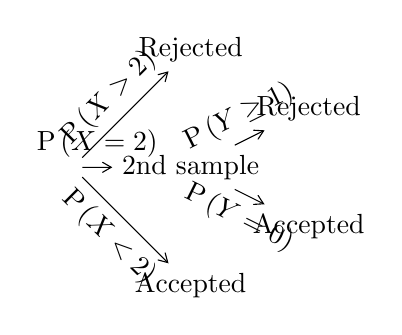
\begin{tikzpicture}[grow=right,->,>=angle 60,sloped]
%\begin{scope}[yshift=0]
 \node {}
    child {node {Accepted}
            edge from parent
            node[below]  {$\text{P}\left(X<2\right)$}
    }
    child {node {2nd sample}
      child {node{Accepted}
       edge from parent
            node[below]  {$\text{P}\left(Y=0\right)$}
        }
      child {node {Rejected}
            edge from parent
            node[above]  {$\text{P}\left(Y\geq 1\right)$}
		}
        edge from parent
            node[above]  {$\text{P}\left(X=2\right)$}
    }
    child {node {Rejected}
        edge from parent
            node[above]  {$\text{P}\left(X>2\right)$}
};

%\end{scope}
\end{tikzpicture}
\end{center}

\begin{enumerate}[label=(\alph*)]


\item  $X\sim\text{no. of pastries by junior chef that do not meet the passing standard, out of 12}$

$X\sim\text{B}\left(12,0.04\right)$

$
\begin{aligned}[t]
\text{P}\left(\text{accepted from the inspection of the 1st sample }\right) & =\text{P}\left(X<2\right)\\
 & =\text{P}\left(X\leq1\right)\\
 & =0.919\text{ (3 s.f.)}
\end{aligned}
$

\item  $Y\sim\text{no. of pastries by junior chef that do not meet the passing standard, out of 8}$

$Y\sim\text{B}\left(8,0.04\right)$

$
\begin{aligned}[t]
\text{P}\left(\text{2nd sample is selected for inspection and rejected}\right) & =\text{P}\left(X=2\right)\times\text{P}\left(Y\geq1\right)\\
 & =\text{P}\left(X=2\right)\times\left[1-\text{P}\left(Y=0\right)\right]\\
 & =0.0196\text{ (3 s.f.)}
\end{aligned}
$


\item
$
\begin{aligned}[t]
\text{P}\left(\text{batch of pastries is rejected}\right) & =\text{P}\left(X>2\right)+\text{P}\left(X=2\right)\times\text{P}\left(Y\geq1\right)\\
 & =\left[1-\text{P}\left(X\leq2\right)\right]+\text{P}\left(X=2\right)\times\left[1-\text{P}\left(Y=0\right)\right]\\
 & =0.0303\text{ (3 s.f.)}
\end{aligned}
$

\item
\begin{enumerate}[label=(\roman*)]

\item  $W\sim\text{no. of pastries by senior chef that do not meet passing standard, out of 6}$

$W\sim\text{B}\left(6,0.025\right)$

$
\begin{aligned}[t]
 & \text{P}\left(\text{exactly 2 pastries do not meet passing standard}\right)\\
 & =\text{P}\left(Y=2\right)\times\text{P}\left(W=0\right)+\text{P}\left(Y=0\right)\times\text{P}\left(W=2\right)+\text{P}\left(Y=1\right)\times\text{P}\left(W=1\right)\\
 & =0.0680\text{ (3 s.f.)}
\end{aligned}
$

\item
$
\begin{aligned}[t]
\text{P}\left(\text{a pastry does not meet the passing standard}\right) & =0.4\left(0.04\right)+0.6\left(0.025\right)\\
 & =0.31
\end{aligned}
$

$A\sim\text{no. of pastries that do not meet the passing standard, out of 20}$

$A\sim\text{B}\left(20,0.031\right)$

$
\begin{aligned}[t]
\text{P}\left(\text{more than 3 do not meet the passing standard}\right) & =\text{P}\left(A>3\right)\\
 & =1-\text{P}\left(A\leq3\right)\\
 & =0.00300\text{ (3 s.f.)}
\end{aligned}
$

\end{enumerate}

\end{enumerate}

\end{example}

\chapter{Normal Distribution}
\section{The Normal Distribution}

The normal distribution is the \textbf{most important} distribution
for a continuous random variable. Many naturally occurring phenomena
have a distribution that is normal, or approximately normal. Some
examples are:

\begin{itemize}

\item  the height of an adult male,

\item  the systolic blood pressure in healthy adults,

\item  the IQ scores of a large population.

\end{itemize}

\centerline{\begin{minipage}{.8\textwidth}

While a discrete random variable is defined by its probability distribution,
a continuous random variable is defined by its \textbf{probability
density function}.

\begin{tcolorbox}[colback=blue!5, colframe=black, boxrule=.4pt, sharpish corners]

If $X$ is normally distributed then its probability density function
is given by
\[
f\left(x\right)=\frac{1}{\sigma\sqrt{2\pi}}e^{-\frac{1}{2}\left(\frac{x-\mu}{\sigma}\right)^{2}}\quad\text{for}\:-\infty<x<\infty
\]
\end{tcolorbox}
\end{minipage}}
\begin{center}
\includegraphics[width=14cm]{\string"lib/Graphics/NormalDistributionCurve\string".png}
\par\end{center}

If $X$ has a normal distribution with mean $\mu$ and variance $\sigma^{2}$
, we write
\[
X\sim\text{N}\left(\mu,\sigma^{2}\right)
\]

\centerline{\begin{minipage}{.8\textwidth}
\begin{tcolorbox}[colback=blue!5, colframe=black, boxrule=.4pt, sharpish corners]

For a normal curve, the standard deviation is uniquely determined
as the horizontal distance from the line of symmetry $x=\mu$ to a
point of inflection.
\end{tcolorbox}
\end{minipage}}

\newpage

\subsection{Properties of The Normal Distribution}

\begin{enumerate}

\item  The curve is bell shaped and \textbf{symmetrical about the
vertical line} $x=\mu$.

\item  The probability of any range of values is given by the \textbf{area
under the pdf} within that interval.

\item  The \textbf{total area} under the pdf curve is $\textbf{1}$.

\end{enumerate}
\begin{center}
\begin{tabular}{>{\centering}p{5cm}>{\centering}p{5cm}>{\centering}p{5cm}}
\centering{}\includegraphics[width=5cm]{\string"lib/Graphics/NormalDistributionCurve4\string".png} & \centering{}\includegraphics[width=5cm]{\string"lib/Graphics/NormalDistributionCurve5\string".png} & \centering{}\includegraphics[width=5cm]{\string"lib/Graphics/NormalDistributionCurve6\string".png}\tabularnewline
$\text{P}\left(X\leq a\right)$ & $\text{P}\left(X\geq a\right)$ & $\text{P}\left(a\leq X\leq b\right)$\tabularnewline
\end{tabular}
\par\end{center}

\begin{center}
\begin{tabular}{>{\centering}p{5cm}>{\centering}p{5cm}>{\centering}p{5cm}}
\centering{}\includegraphics[width=5cm]{\string"lib/Graphics/NormalDistributionCurve2\string".png} & \centering{}\includegraphics[width=5cm]{\string"lib/Graphics/NormalDistributionCurve3\string".png} & \centering{}\includegraphics[width=5cm]{\string"lib/Graphics/NormalDistributionCurve7\string".png}\tabularnewline
${\displaystyle \text{P}\left(X\leq\mu\right)=\frac{1}{2}}$ & ${\displaystyle \text{P}\left(X\geq\mu\right)=\frac{1}{2}}$ & $\text{Total Area}=1$\tabularnewline
\end{tabular}
\par\end{center}

Note: $\text{P}\left(X=a\right)=0$ since the corresponding area under
the curve is zero. Hence for a normal random variable, we have
\begin{align*}
\text{P}\left(X\leq a\right) & =\text{P}\left(X<a\right)+\text{P}\left(X=a\right)=\text{P}\left(X<a\right)\text{ and similarly,}\\
\text{P}\left(X\geq a\right) & =\text{P}\left(X>a\right)+\text{P}\left(X=a\right)=\text{P}\left(X\geq a\right)
\end{align*}


\subsection{Finding Probabilities Using Graphic Calculator}

For $X\sim\text{N}\left(\mu,\sigma^{2}\right)$, using the graphic
calculator: Press \tcbox[box align=base,nobeforeafter,colback=blue!40, colframe=blue!40,size=small]{\textbf{\textcolor{white}{2ND}}}\tcbox[box align=base,nobeforeafter,colback=black, colframe=black,size=small]{\textbf{\textcolor{white}{VARS}}}

\begin{itemize}

\item To find $\text{P}\left(X\leq b\right)$: Select 2:normalcdf
and key the values in the format $10^{-99}$, $b$, $\mu$, $\sigma$.

\item  To find $\text{P}\left(X\geq a\right)$: Select 2:normalcdf
and key the values in the format $a$, $10^{99}$, $\mu$, $\sigma$.

\item  To find $\text{P}\left(a\leq X\leq b\right)$: Select 2:normalcdf
and key the values in the format $a$, $b$, $\mu$, $\sigma$.

\item  To find $a$ such that $\text{P}\left(X\leq a\right)=p$ :
Select 3:invNorm and key the values in the format $p$, $\mu$, $\sigma$,
tail.

\end{itemize}

Note: Remember to enter $\sigma$ (standard deviation) and not $\sigma^{2}$
(variance) when using the GC.

\begin{example}[Finding Probabilities of Normal Distributions (Area Under The Curve)]

The weight of a randomly chosen student from a population may be assumed
to have a normal distribution with mean $65\,\text{kg}$ and standard
deviation $3\,\text{kg}$. A student was randomly chosen from this
population. Find the proabability that

\begin{enumerate}[label=(\alph*)]

\item  his weight exceeds $\text{70}\,\text{kg}$,

\item  his weight is below $\text{62}\,\text{kg}$,

\item  his weight is between $60\,\text{kg}$ and $75\,\text{kg}$,

\item  his weight is within one standard deviation from the mean
weight.

\end{enumerate}

\Solution

Let $X$ be the weight of a randomly chosen student

$X\sim\text{N}\left(65,9\right)$

\begin{enumerate}[label=(\alph*)]

\item  $\text{P}\left(X>70\right)=0.478\text{ (3 s.f.)}$

\item  $\text{P}\left(X<62\right)=0.159\text{ (3 s.f.)}$

\item  $\text{P}\left(60<X<75\right)=0.952\text{ (3 s.f.)}$

\item
$
\begin{aligned}[t]
\text{P}\left(\left|X-65\right|<3\right) & =\text{P}\left(62<X<68\right)\\
 & =0.683\text{ (3 s.f.)}
\end{aligned}
$

\end{enumerate}

\end{example}

\begin{example}[Inverse Normal Values]

Given $X\sim\text{N}\left(10,4\right)$, find, correct to 3 significant
figures, the values of $a$, $b$ and $c$ such that

\begin{enumerate}[label=(\alph*)]

\item  $\text{P}\left(X\leq a\right)=0.15$

\item  $\text{P}\left(X\geq b\right)=0.23$

\item  $\text{P}\left(9<X<c\right)=0.64$

\end{enumerate}

\Solution

\begin{enumerate}[label=(\alph*)]

\item

\begin{minipage}[t]{.6\textwidth}

From GC, $a=7.93\text{ (3 s.f.)}$

\includegraphics[width=4cm]{\string"lib/GC Screenshots/invNorm1\string".png}\hspace{1cm}\includegraphics[width=4cm]{\string"lib/GC Screenshots/invNorm2\string".png}

\end{minipage}
\begin{minipage}[t]{.3\textwidth}
\begin{center}
\includegraphics[width=5cm,valign=t]{\string"lib/Graphics/NormalExInvNorm1\string".png}
\par\end{center}

\end{minipage}

\item  \begin{minipage}[t]{.6\textwidth}

From GC, $b=11.5\text{ (3 s.f.)}$

\includegraphics[width=4cm]{\string"lib/GC Screenshots/invNorm3\string".png}\hspace{1cm}\includegraphics[width=4cm]{\string"lib/GC Screenshots/invNorm4\string".png}

\end{minipage}
\begin{minipage}[t]{.3\textwidth}
\begin{center}
\includegraphics[width=5cm,valign=t]{\string"lib/Graphics/NormalExInvNorm2\string".png}
\par\end{center}

\end{minipage}

\item
$
\begin{aligned}[t]
\text{P}\left(X<c\right)-\text{P}\left(X<9\right) & =0.64\\
\text{P}\left(X<c\right) & =0.64+\text{P}\left(X<9\right)\\
 & =0.94854\text{ (5 s.f.)}
\end{aligned}
$

\begin{minipage}[t]{.6\textwidth}

From GC, $c=13.3\text{ (3 s.f.)}$

\includegraphics[width=4cm]{\string"lib/GC Screenshots/invNorm5\string".png}\hspace{1cm}\includegraphics[width=4cm]{\string"lib/GC Screenshots/invNorm6\string".png}

\end{minipage}
\begin{minipage}[t]{.3\textwidth}
\begin{center}
\includegraphics[width=5cm,valign=t]{\string"lib/Graphics/NormalExInvNorm3\string".png}
\par\end{center}

\end{minipage}

\end{enumerate}

\end{example}

\section{The Standard Normal Distribution (Z-Distribution)}

The standard normal distribution with mean $\mu=0$ and standard deviation $\sigma=1$ is denoted by $Z$, i.e.

$Z\sim\text{N}\left(0,1\right)$.

Every normal distribution can be transformed into the standard normal
distribution or $Z-$distribution using the transformation ${\displaystyle Z=\frac{X-\mu}{\sigma}}$.

This process of converting $X\sim\text{N}\left(\mu,\sigma^{2}\right)$
into $Z\sim\text{N}\left(0,1\right)$ is known as standardisation.

We usually perform standardisation when $\mu$ and/or $\sigma$ are
unknown.

\begin{example}[Standardisation to Find $\mu$]

Given that $X\sim\text{N}\left(\mu,0.04\right)$ and $\text{P}\left(X<5\right)=0.3$,
find $\mu$.

\Solution

\begin{align*}
\text{P}\left(X<5\right) & =0.3\\
\text{P}\left(Z<\frac{5-\mu}{\sqrt{0.04}}\right) & =0.3
\end{align*}

From GC,
\begin{align*}
\frac{5-\mu}{0.2} & =-0.52440\text{ (5 s.f.)}\\
\mu & =5.10\text{ (3 s.f.)}
\end{align*}

\end{example}

\begin{example}[Standardisation to Find $\sigma$]

Given that $X\sim\text{N}\left(12,\sigma^{2}\right)$ and $\text{P}\left(X\geq15\right)=0.0668$,
find the standard deviation of $X$.

\Solution

\begin{align*}
\text{P}\left(X\geq15\right) & =0.0668\\
\text{P}\left(Z<\frac{15-12}{\sigma}\right) & =0.0668
\end{align*}

From GC,
\begin{align*}
\frac{3}{\sigma} & =1.5001\text{ (5 s.f.)}\\
\sigma & =2.00\text{ (3 s.f.)}
\end{align*}

\end{example}

\newpage

\begin{example}[Standardisation to Find $\mu$ and $\sigma$]

In a particular town, $34$ out of $100$ people have heights exceeding
$1.65\,\text{m}$ and $4$ out of $5$ people have heights below $1.8\,\text{m}$.
Assuming that their heights follow a normal distribution, find the
mean and standard deviation of the distribution.

\Solution

Let $X$ be the height of a randomly chosen person from the town.

$X\sim\text{N}\left(\mu,\sigma^{2}\right)$

Given that $\text{P}\left(X>1.65\right)=0.34$,

\begin{align*}
\text{P}\left(X>1.65\right) & =0.34\\
\text{P}\left(Z>\frac{1.65-\mu}{\sigma}\right) & =0.34\\
\text{P}\left(Z\leq\frac{1.65-\mu}{\sigma}\right) & =0.66\\
\frac{1.65-\mu}{\sigma} & =0.41246\text{ (5 s.f.)}
\end{align*}

and given that $\text{P}\left(X<1.8\right)=0.8$,
\begin{align*}
\text{P}\left(X<1.8\right) & =0.8\\
\text{P}\left(Z<\frac{1.8-\mu}{\sigma}\right) & =0.8\\
\frac{1.8-\mu}{\sigma} & =0.84162\text{ (5 s.f.)}
\end{align*}

Rearranging the equations, we have the following simultaneous equations:

\begin{align*}
\mu+0.41246\sigma & =1.65\cdots\cdots(1)\\
\mu+0.84162 & =1.8\cdots\cdots(2)
\end{align*}

Using GC to solve (1) and (2), $\mu=1.51$ and $\sigma=0.350$.

\end{example}

\newpage

\section{Linear Combinations of Normal Random Variables}

Recall that we have the following properties for the expectation and
variance of two random variables.

\medskip

\centerline{\begin{minipage}{\textwidth}
\begin{tcolorbox}[colback=blue!5, colframe=black, boxrule=.4pt, sharpish corners]

For any random variables $X$ and $Y$, and constants $a$ and $b$,

\medskip{}

\begin{minipage}[t]{0.5\textwidth}

\begin{enumerate}[label=(\alph*)]

\item  $\text{E}\left(a\right)=a$

\item  $\text{E}\left(aX\right)=a\text{E}\left(X\right)$

\item  $\text{E}\left(aX\pm b\right)=a\text{E}\left(X\right)\pm b$

\item  $\text{E}\left(aX\pm bY\right)=a\text{E}\left(X\right)\pm b\text{E}\left(Y\right)$

\end{enumerate}

\end{minipage}
\begin{minipage}[t]{0.5\textwidth}

\begin{enumerate}[label=(\alph*)]

\item  $\text{Var}\left(a\right)=0$

\item $\text{Var}\left(aX\right)=a^{2}\text{Var}\left(X\right)$

\item $\text{Var}\left(aX\pm b\right)=a^{2}\text{Var}\left(X\right)$

\item  If $X$ and $Y$ are \textbf{independent}, then

$\text{Var}\left(aX\pm bY\right)=a^{2}\text{Var}\left(X\right)+b^{2}\text{Var}\left(Y\right)$

\end{enumerate}

\end{minipage}
\end{tcolorbox}
\end{minipage}}

\medskip


If $X$ and $Y$ are two \textbf{independent normal} random variables,
and $a$ and $b$ are non zero constants, then

\[
aX\pm bY\:\text{are also normal random variables.}
\]

Thus, if $X\sim\text{N}\left(\mu_{1},\sigma_{1}^{2}\right)$ and $Y\sim\text{N}\left(\mu_{2},\sigma_{2}^{2}\right)$
are independent random variables, and $a$ and $b$ are non zero constants,
then

\begin{enumerate}[label=(\alph*)]

\item $aX\sim\text{N}\left(a\mu_{1},a^{2}\sigma_{1}^{2}\right)$

\item $aX\pm b\sim\text{N}\left(a\mu_{1}\pm b,a^{2}\sigma_{1}^{2}\right)$

\item $aX\pm bY\sim\text{N}\left(a\mu_{1}\pm b\mu_{2},a^{2}\sigma_{1}^{2}+b^{2}\sigma_{2}^{2}\right)$

\end{enumerate}

\begin{example}[Finding Distribution of Linear Combinations of Normal Random Variables]

Given $X$ and $Y$ are independent with $X\sim\text{N}\left(3,9\right)$
and $Y\sim\text{N}\left(1,4\right)$

State the distribution of:

\begin{tasks}[label=(\alph*),label-width=3.5ex](2)

\task  $2X$

\task  $X+3$

\task  $X+2Y$

\task  $X-2Y$

\task  $X_{1}+X_{2}+X_{3}+Y_{1}+Y_{2}$, where $X_{1},X_{2},X_{3}$
are independent observations of $X$ and $Y_{1},Y_{2}$ independent
observations of $Y$.

\end{tasks}

\Solution

\begin{tasks}[label=(\alph*),label-width=3.5ex](2)

\task  $2X\sim\text{N}\left(6,36\right)$

\task  $X+3\sim\text{N}\left(6,9\right)$

\task  $X+2Y\sim\text{N}\left(5,25\right)$

\task  $X-2Y\sim\text{N}\left(1,25\right)$

\task  $X_{1}+X_{2}+X_{3}+Y_{1}+Y_{2}\sim\text{N}\left(11,35\right)$

\end{tasks}

\end{example}

\newpage

\begin{example}[Heights of Males vs Females]

In a particular town, the heights, in centimetres, of the males and
females are normally distributed as follows:
\begin{center}
\setlength{\extrarowheight}{2pt}%
\begin{tabular}{|>{\centering}p{4cm}|>{\centering}p{4cm}|>{\centering}p{4cm}|}
\hline
 & Mean & Standard Deviation\tabularnewline
\hline
Male & $177$ & $18.4$\tabularnewline
\hline
Female & $162$ & $13.2$\tabularnewline
\hline
\end{tabular}
\par\end{center}

\begin{enumerate}[label=(\alph*)]

\item  Find the probability that a randomly chosen female is taller
than a randomly chosen male.

\item  Find the probability that the total height of three randomly
chosen females exceeds that of $2$ randomly chosen males by more
than $100\,\text{cm}$.

\end{enumerate}

\Solution

Let $X$ be the height of a randomly chosen male from the town.

$X\sim\text{N}\left(177,18.4^{2}\right)$

Let $Y$ be the height of a randomly chosen female from the town.

$Y\sim\text{N}\left(162,13.2^{2}\right)$

\begin{enumerate}[label=(\alph*)]

\item  $Y-X\sim\text{N}\left(-15,512.8\right)$

\begin{align*}
\text{P}\left(Y>X\right) & =\text{P}\left(Y-X>0\right)\\
 & =0.254\text{ (3 s.f.)}
\end{align*}

\item  $\left(Y_{1}+Y_{2}+Y_{3}\right)-\left(X_{1}+X_{2}\right)\sim\text{N}\left(132,1199.84\right)$

\[
\text{P}\left(Y_{1}+Y_{2}+Y_{3}-X_{1}+X_{2}>100\right)=0.822\text{ (3 s.f.)}
\]

\end{enumerate}

\end{example}

\begin{example}[Mass of Papayas]

Papayas are sold by mass. The masses, in kg, of papayas follow a normal distribution with mean $0.7$ and standard deviation $6.1$.

Find the probability that the total mass of $2$ randomly chosen papayas
is heavier than twice the mass of a randomly chosen papaya by at most
$80\,\text{g}$.

\Solution

Let $X$ be the mass of a randomly chosen papaya

$X\sim\text{N}\left(0.7,6.1^{2}\right)$

$\left(X_{1}+X_{2}\right)-2X\sim\text{N}\left(0,223.26\right)$

\[
\text{P}\left(X_{1}+X_{2}-2X<0.08\right)=0.502\text{ (3 s.f.)}
\]

\end{example}

\newpage{}



\chapter{Sampling Distribution (Central Limit Theorem)}

\section{Population and Sample}

When we need to gather information about a \textbf{population}, very
rarely in practice can we afford the luxury of examining the complete
population. The two obvious reasons would be that the cost is too
high and the population is dynamic in that the individuals making
up the population may change over time.

Commonly, \textbf{sample} observations and analyses are used to make inferences or predictions about a population. That is, we take the
results of an analysis using a sample and generalize it to the larger
population that the sample represents. This is known as \textit{statistical inference}.

\medskip

\centerline{\begin{minipage}{.68\textwidth}
\begin{tcolorbox}[colback=blue!5, colframe=black, boxrule=.4pt, sharpish corners]

A \textbf{population} is the whole set of items that we want to study.

A \textbf{sample} is a subset of the population.
\end{tcolorbox}
\end{minipage}}

\medskip


In order for the statistical inference to be as accurate as possible,
however, it is imperative that the sample is representative of the
population (i.e. accurately reflect the characteristics of the population)
to which it is being generalized. As such, the sample must be carefully
gathered through \textbf{random sampling}.

\section{Random Sampling}

\centerline{\begin{minipage}{.68\textwidth}
\begin{tcolorbox}[colback=blue!5, colframe=black, boxrule=.4pt, sharpish corners]

In \textbf{random sampling}, every element in the population must
have an equal chance of selection, i.e. it is free from bias.
\end{tcolorbox}
\end{minipage}}

\medskip

In non-random sampling, each element in the population does not have
an equal chance of being selected, resulting in certain segments of
the population being over represented, as some members are systematically or deliberately excluded from study.

\begin{example}[Random Sampling Methods]

In a small school there are 3 classes, each with 30 students, and
2 classes, each with 20 students. To find the students perception
of the food sold in a canteen, a sample of 10 students is taken by
the following three methods.

\begin{enumerate}[label=Method \arabic*:, leftmargin=2cm]

\item  2 students are randomly chosen from each of the 5 classes.

\item  Assign every student in the school with a number from 1 to
130 by arranging their names in alphabetical order. Use a computer
to generate 10 random numbers. The 10 students with the corresponding
numbers would be the ones chosen to be in the sample.

\item  The first 10 students who patrionize the chicken rice stall
are selected as the sample.

\end{enumerate}

\Solution

In choosing a random sample, each member of the population must have an equal chance of being selected.

\uline{Method 1}

Let $A$ be the event that a particular student from the class of
$20$ is chosen.

\begin{align*}
\text{P}\left(A\right) & =\frac{1}{10}
\end{align*}

Let $B$ be the event that a particular student from the class of
$30$ is chosen.
\begin{align*}
\text{P}\left(B\right) & =\frac{1}{15}
\end{align*}
Since the probability of choosing any one student is not equal, this
method does not involve random sampling.

\uline{Method 2}

Since each student has a probability of ${\displaystyle \frac{1}{13}}$
of being chosen, this method does involve random sampling.

\uline{Method 3}

This method does not involve random sampling because students who
do not eat chicken rice will not patrionize the chicken rice stall
and thus will not be selected.

\end{example}

\section{Population Parameters and Sample Statistics}

\centerline{\begin{minipage}{.65\textwidth}
\begin{tcolorbox}[colback=blue!5, colframe=black, boxrule=.4pt, sharpish corners]

A \textbf{population parameter} is a number that is characteristic
of the population under study.
\end{tcolorbox}
\end{minipage}}

\medskip

A population parameter is a number that is characteristic of the population under study.

In many cases, we are concerned with two population parameters,

\begin{itemize}

\item  \textbf{population mean }

\item  \textbf{population variance}

\end{itemize}

These are constants of a population and they are often unknown. The
study of a population often involves finding estimates of these parameters.

\medskip

\centerline{\begin{minipage}{.6\textwidth}
\begin{tcolorbox}[colback=blue!5, colframe=black, boxrule=.4pt, sharpish corners]

A \textbf{sample statistic} is a number that is characteristic of
a sample drawn from the population.
\end{tcolorbox}
\end{minipage}}

\medskip

In general, a sample statistic is a \textbf{random variable} which
contains information about the sample while any corresponding population parameter is a (possibly unknown) constant.

We use the following notation for parameters and statistics.\setlength{\extrarowheight}{2pt}

\begin{tabular}{|>{\centering}m{3.5cm}|>{\centering}m{3.5cm}|>{\centering}m{3.5cm}|>{\centering}m{3.5cm}|}
\hline
\multirow{2}{3.5cm}{\hspace{31bp}Quantity} & \multirow{2}{3.5cm}{\hspace{25bp}Population} & \multicolumn{2}{c|}{Sample}\tabularnewline
\cline{3-4} \cline{4-4}
 &  & As a random variable & As a possible value\tabularnewline
\hline
Mean & $\mu$ & $\overline{X}$ & $\overline{x}$\tabularnewline
\hline
Variance & $\sigma^{2}$ & $\sigma_{X}^{2}$ & $\sigma_{x}^{2}$\tabularnewline
\hline
\end{tabular}

\newpage


\section{The Sample Mean, $\textbf{\ensuremath{\overline{X}}}$ as a Random Variable}

Let $X_{1},X_{2},X_{3},...,X_{n}$ be $n$ independent observations
taken from a population $X$, with mean $\mu$ and variance $\sigma^{2}$.

Then the sample mean $\overline{X}$, defined by
\[
\overline{X}=\frac{X_{1}+X_{2}+X_{3}+\ldots+X_{n}}{n}
\]
is a random variable with $\text{E}\left(\overline{X}\right)=\mu$
and ${\displaystyle \text{Var}\left(\overline{X}\right)=\frac{\sigma^{2}}{n}}$.

\begin{fleqn}

\textbf{Proof}:

\begin{minipage}[t]{0.5\textwidth}

\begin{align*}
\text{E}\left(\overline{X}\right) & =\text{E}\left(\frac{X_{1}+X_{2}+X_{3}+\ldots+X_{n}}{n}\right)\\
 & =\frac{1}{n}\text{E}\left(X_{1}+X_{2}+X_{3}+\ldots+X_{n}\right)\\
 & =\frac{1}{n}\left(n\text{E}\left(X\right)\right)\\
 & =\mu
\end{align*}

\end{minipage}
\hfill\vline\hfill
\begin{minipage}[t]{0.5\textwidth}

$
\begin{aligned}[t]
\text{Var}\left(\overline{X}\right) & =\text{Var}\left(\frac{X_{1}+X_{2}+X_{3}+\ldots+X_{n}}{n}\right)\\
 & =\frac{1}{n^{2}}\text{Var}\left(X_{1}+X_{2}+X_{3}+\ldots+X_{n}\right)\\
 & =\frac{1}{n^{2}}\left(n\text{Var}\left(X\right)\right)\\
 & =\frac{\sigma^{2}}{n}
\end{aligned}
$

\end{minipage}

\end{fleqn}

\section{Distribution of $\textbf{\ensuremath{\overline{X}}}$ }

\subsection{When $X$ Follows a Normal Distribution}

\begin{tcolorbox}[colback=blue!5, colframe=black, boxrule=.4pt, sharpish corners]

If $X_{1},X_{2},X_{3},...,X_{n}$ are $n$ independent observations
from a \textbf{normal distribution} with mean $\mu$ and variance
$\sigma^{2}$, then the sample mean $\overline{X}$ is also normally
distributed such that
\[
\overline{X}\sim\text{N}\left(\mu,\frac{\sigma^{2}}{n}\right)\:\textbf{exactly}
\]

\end{tcolorbox}

\begin{example}[Sample Mean of a Normal Distribution]

A random sample of size $15$ is taken from a population which is
normally distributed with mean $60$ and standard deviation $4$.
Find the probability that the mean of the sample is less than $58$.

\Solution

Let ${\displaystyle X\sim\text{N}\left(60,4^{2}\right)}$

${\displaystyle \overline{X}\sim\text{N}\left(60,\frac{4^{2}}{15}\right)}\:\text{exactly}$

Using GC,
\[
\text{P}\left(\overline{X}<58\right)=0.0264
\]
\end{example}

\newpage

\begin{example}[Finding $n$ By Standardization]

A large number of random samples of size $n$ are taken from a normal
population with mean 74 and variance 36 and the sample means are calculated.
If at most $85\%$ of the sample means exceed $72$, find the largest
possible value of $n$.

\Solution

Let ${\displaystyle X\sim\text{N}\left(74,36\right)}$

${\displaystyle \overline{X}\sim\text{N}\left(74,\frac{36}{n}\right)}\:\text{exactly}$

Given $\text{P}\left(\overline{X}>72\right)\leq0.85$,

\begin{align*}
\text{P}\left(Z>\frac{72-74}{\sqrt{\frac{36}{n}}}\right) & \leq0.85\\
\text{P}\left(Z>-\frac{\sqrt{n}}{3}\right) & \leq0.85\\
-\frac{\sqrt{n}}{3} & \leq-1.0364(\text{5 s.f.})\\
n & \leq9.67(\text{3 s.f.})
\end{align*}
Thus the largest possible value of $n$ is $9$.

\end{example}

\subsection{When $X$ Follows Any Distribution (Central Limit Theorem)}

\begin{tcolorbox}[colback=blue!5, colframe=black, boxrule=.4pt, sharpish corners]

If $X_{1},X_{2},X_{3},...,X_{n}$ are $n$ independent observations
from \textbf{ANY distribution}, $\boldsymbol{X}$, with mean $\mu$ and variance
$\sigma^{2}$, then when $n$ is sufficiently large $\left(n\geq30\right)$,
by the \textbf{Central Limit Theorem},
\[
\overline{X}\sim\text{N}\left(\mu,\frac{\sigma^{2}}{n}\right)\:\textbf{approximately}
\]

\end{tcolorbox}

\begin{example}[Sample Mean of a Binomial Distribution Using CLT]

Ten fair die are thrown and the number of sixes is recorded. If the
experiment is repeated $50$ times and the number of sixes are recorded
each time, estimate the probability that the mean number of sixes
in each experiment will be less than $1.6$.

\Solution
Let $X$ be the no. of sixes out of 10 fair die.

${\displaystyle X\sim\text{B}\left(10,\frac{1}{6}\right)}$

\begin{align*}
\text{E}\left(X\right) & =np=\frac{5}{3}\qquad\qquad\text{Var}\left(X\right)=np\left(1-p\right)=\frac{25}{18}
\end{align*}

Since the sample size $n=50$ is sufficiently large $\left(\geq30\right)$,
by the Central Limit Theorem,
\[
\overline{X}\sim\text{N}\left(\frac{5}{3},\frac{1}{36}\right)\:\text{approximately}
\]

Thus,
\[
\text{P}\left(\overline{X}<1.6\right)=0.345(\text{3 s.f.})
\]
\end{example}

\begin{example}[Sample Mean of a Probability Distribution Using CLT]

A random variable $X$ has the probability distribution shown in the
table below. The sample mean for 50 independent observations of $X$
is denoted by $\overline{X}$. Using a suitable approximation, find
$\text{P}\left(\overline{X}>0\right)$.
\begin{center}
\begin{tabular}{|>{\centering}m{2cm}|>{\centering}m{2cm}|>{\centering}m{2cm}|>{\centering}m{2cm}|>{\centering}m{2cm}|>{\centering}m{2cm}|}
\hline
$x$ & $-2$ & $-1$ & $0$ & $1$ & $2$\tabularnewline
\hline
$\text{P}\left(X=x\right)$ & $0.3$ & $0.1$ & $0.15$ & $0.4$ & $0.05$\tabularnewline
\hline
\end{tabular}
\par\end{center}

\Solution

\begin{align*}
\text{E}\left(X\right) & =-2\left(0.3\right)-1\left(0.1\right)+0+1\left(0.4\right)+2\left(0.05\right)\\
 & =-0.2
\end{align*}
\begin{align*}
\text{E}\left(X^{2}\right) & =4\left(0.3\right)+1\left(0.1\right)+0+1\left(0.4\right)+4\left(0.05\right)\\
 & =1.9
\end{align*}

\begin{align*}
\text{Var}\left(X\right) & =\text{E}\left(X^{2}\right)-\left[\text{E}\left(X\right)\right]^{2}\\
 & =1.86
\end{align*}
Since the sample size $n=50$ is sufficiently large $\left(\geq30\right)$,
by the Central Limit Theorem,
\[
\overline{X}\sim\text{N}\left(-0.2,\frac{1.86}{50}\right)\:\text{approximately}
\]
\[
\text{P}\left(\overline{X}>0\right)=0.150(\text{3 s.f.})
\]

\end{example}


\section*{Central Limit Theorem Summary}


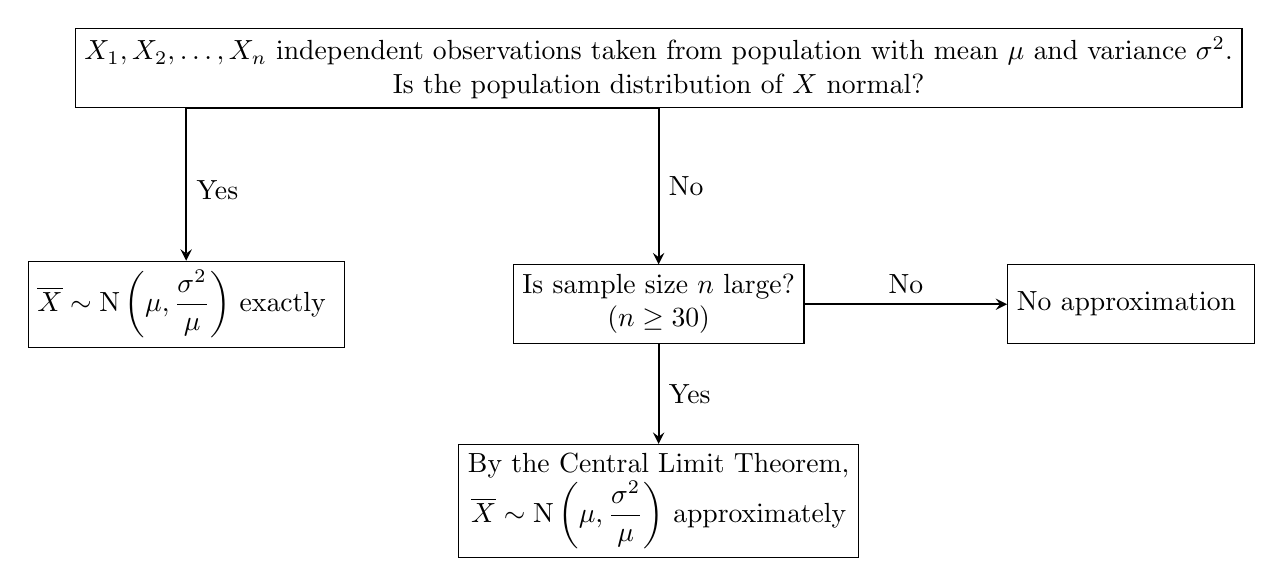
\begin{tikzpicture}[every text node part/.style={align=center}]
\node (Population Distribution)[Box]{$X_{1},X_{2},\ldots,X_{n}$ independent observations taken from population with mean $\mu$ and variance $\sigma^{2}$.\\

Is the population distribution of $X$ normal?
};
\node (Not Exact)[Box, below of = Population Distribution, yshift=-2cm]{Is sample size $n$ large? \\
$\left(n\geq30\right)$
};

\node (Exact)[Box, left of = Not Exact,xshift=-5cm]{${\displaystyle \overline{X}\sim\text{N}\left(\mu,\frac{\sigma^{2}}{\mu}\right)}$
exactly
};

\node (Not large)[Box, right of = Not Exact,xshift=5cm]{ No approximation
};

\node (CLT)[Box, below of = Not Exact,yshift=-1.5cm]{ By the Central Limit Theorem,  \\

$
{\displaystyle \overline{X}\sim\text{N}\left(\mu,\frac{\sigma^{2}}{\mu}\right)}\text{ approximately}
$
};


\draw[arrow](Population Distribution)--(Not Exact)node[midway, right]{No};
\draw[arrow](Population Distribution.south)-|(Exact.north)node[right,yshift=.9cm]{Yes};
\draw[arrow](Not Exact.east)--(Not large.west)node[midway,above]{No};
\draw[arrow](Not Exact.south)--(CLT.north)node[midway,right]{Yes};



\end{tikzpicture}


\chapter{Hypothesis Testing}
\vspace{-1cm}
\begin{investigation}[colbacktitle=myblue]{Opening Problem}

A manufacturer claims that the light bulbs he produces have a mean
lifespan of $600$ hours, and a standard deviation of $60$ hours.
In statistics, we call this a \textbf{statistical hypothesis}.

A retailer, having received numerous complaints from his customers,
suspects that they do not last as long. He contacts the manufacturer
and they decide to test a random sample of $50$ bulbs. It turns out
that the average lifespan of this sample, $\overline{x}$, is $580$
hours.

\begin{minipage}[t]{.65\textwidth}

Is this proof that the average lifespan of their light bulbs is below
$600$ hours? It is possible that the average lifespan of the population
is actually $600$ and that the sampled light bulbs just had a lower
than average lifespan. Our sample cannot tell us with certainty the
exact population mean $\mu$. How do we then decide between the validity of manufacturer's claim and that of the angry customers?

\medskip

Statisticians have devised a procedure to determine whether a statistical hypothesis is reasonable. We call it a \textbf{hypothesis test}.

\end{minipage}
\begin{minipage}[t]{.35\textwidth}
\begin{center}
\includegraphics[width=5cm,valign=t]{\string"lib/Graphics/ManLooksAtLightBulb\string".png}
\par\end{center}

\end{minipage}
\end{investigation}

\medskip

\centerline{\begin{minipage}{.94\textwidth}
\begin{tcolorbox}[colback=blue!5, colframe=black, boxrule=.4pt, sharpish corners]

A \textbf{statistical hypothesis} is an assertion or conjecture\footnotemark
concerning one or more populations.
\end{tcolorbox}
\end{minipage}}

\footnotetext{An opinion or conclusion formed on the basis of incomplete information.}

\medskip

To prove that a hypothesis is true, or false, with absolute certainty,
we would need absolute knowledge. That is, we would have to examine
the entire population. In most cases, it would not make sense to examine the entire population. For example if the light bulb manufacturer were to test the lifespan every light bulb he produces, he would have no light bulbs left to sell. Instead, hypothesis testing concerns on how to use a random sample to judge if it is evidence that supports or not the hypothesis.

\section{Null and Alternative Hypotheses}

Suppose a claim is made that a population mean $\mu$ has a value
$\mu_{0}$. We call this the \textbf{null hypothesis} $H_{0}$, and
we write
\[
H_{0}:\mu=\mu_{0}
\]

This statement is assumed to be true unless we have enough evidence
to reject it.

The alternative hypothesis, denoted by $H_{1}$, is used to contradict
the null hypothesis.

\medskip

\begin{tcolorbox}[colback=blue!5, colframe=black, boxrule=.4pt, sharpish corners]

Given the null hypothesis $H_{0}:\mu=\mu_{0}$, there are three ways to set up the alternative hypothesis:

\begin{itemize}
  \item $H_{1}:\mu>\mu_{0}$

  \item $H_{1}:\mu<\mu_{0}$
	\makebox(0,0){\put(0,3\normalbaselineskip){%
            $\left.\rule{0pt}{1.4\normalbaselineskip}\right\}$ \textbf{One-tail Test}}}
  \item $H_{1}:\mu\neq\mu_{0}$ \hspace{.33cm} \textbf{Two-tail Test}

\end{itemize}
\end{tcolorbox}

\newpage

Consider the \textbf{Opening Problem}. The manufacturer
claims (null hypothesis) that his light bulbs have a lifespan of $600$
hours. We write, $H_{0}:\mu=600$.

The retailer's suspicion that this claim is over-estimated (alternative
hypothesis) is written formally as $H_{1}:\mu<600$.

\begin{example}[Null and Alternative Hypothesis]

For each of the following scenarios, write down the null and alternative
hypotheses. State whether a one-tail or two tail test applies.

\begin{enumerate}[label=(\alph*)]

\item  The top speed of submarines currently being produced by a
manufacturer is currently $26.3$ knots. When their engineers modify
the design to reduce drag, they believe the maximum speed will be
increased.

\item  The average peak-hour travel time along a particular stretch
of road is currently $27$ minutes. To help reduce travel times, electronic
signs displaying real-time information are erected. If the travel
times improve, the signs will be widely implemented.

\item  Whitex produces copy paper, and the weight of the copy paper
is given as $80\,\text{g per m}^{2}$. The company wants to determine
whether this information is correct.

\end{enumerate}

\Solution

\begin{tasks}[label=(\alph*),label-width=3.5ex](3)

\task  $H_{0}:\mu=26.3$, $H_{1}:\mu>26.3$

One-tail test

\task  $H_{0}:\mu=27$, $H_{1}:\mu<27$

One-tail test

\task  $H_{0}:\mu=80$, $H_{1}:\mu\neq80$

Two-tail test

\end{tasks}

\end{example}

\section{Hypothesis Testing}

\subsection{The Test Statistic}

To carry out the test, our focus moves from $X$ (e.g. the lifespan
of light bulbs) to the distribution of $\overline{X}$ (e.g. the mean
lifespan from a sample of lightbulbs). $\overline{X}$ is called the
\textbf{test statistic} for the population mean $\mu$. The decision
to reject or not to reject $H_{0}$ depends on how far the observed
sample mean, $\overline{x}$, is from the claimed mean.

\begin{tcolorbox}[colback=blue!5, colframe=black, boxrule=.4pt, sharpish corners]

A \textbf{test statistic} is a random variable that is calculated
from sample data (e.g. sample mean).

\medskip

The distribution of the test statistic under the assumptions of $H_{0}$
is called the \textbf{null distirbution}.
\end{tcolorbox}

We have seen that for a population which is normally distributed with
mean $\mu$ and standard deviation $\sigma$, the sample mean

\[
\overline{X}\sim\text{N}\left(\mu,\frac{\sigma^{2}}{n}\right)\text{ exactly}
\]

If the population is not normally distributed but the sample size
is sufficiently large, we can apply the Central Limit Theorem

\[
\overline{X}\sim\text{N}\left(\mu,\frac{\sigma^{2}}{n}\right)\text{ approximately}
\]

Under the assumptions of $H_{0}$, $\mu=\mu_{0}$, so our null distribution
is ${\displaystyle \overline{X}\sim\text{N}\left(\mu_{0},\frac{\sigma^{2}}{n}\right)}$.

In our light bulb example, $H_{0}:\mu=600$. Under the assumption
that the null hypothesis is true, the population mean and standard
deviation are $\mu=600$ and $\sigma=60$ (these are the values given
by the manufacturer). Our sample size $n$ is $50$. So, by the Central
Limit Theorem, we have the null distribution

\[
\overline{X}\sim\text{N}\left(600,\frac{60^{2}}{50}\right)\text{ approximately, since \ensuremath{n=50} is sufficiently large}
\]

However in hypothesis testing, we will not be using the test statistic
$\overline{X}$. Instead, the standardised test statistic is used,

\[
Z=\frac{\overline{X}-\mu_{0}}{\frac{\sigma}{\sqrt{n}}},\text{ where }Z\sim\text{N}\left(0,1\right)
\]

\begin{tcolorbox}[colback=blue!5, colframe=black, boxrule=.4pt, sharpish corners]

Consider a statistical hypothesis test of $H_{0}:\mu=\mu_{0}$ for
a normally distributed population with known standard deviation $\sigma$.
Given a sample of size $n$ with observed sample mean $\overline{x}$:

The standardised test statistic is ${\displaystyle Z=\frac{\overline{X}-\mu_{0}}{\frac{\sigma}{\sqrt{n}}}},\text{ where }Z\sim\text{N}\left(0,1\right)$

which has observed value ${\displaystyle z=\frac{\overline{x}-\mu_{0}}{\frac{\sigma}{\sqrt{n}}}}$.
\end{tcolorbox}

Back to the light bulb example:

The population standard deviation is $60$ hours.

When they take a random sample of $50$ light bulbs, they find that
the mean lifespan is $\bar{x}=580$ hours.

The observed value of the test statistic is ${\displaystyle z=\frac{580-600}{\frac{60}{\sqrt{50}}}}\approx-2.36$.

\subsection{Level of Significance}

In hypothesis testing, the null hypothesis may be rejected (or not
rejected) not with certainty but with confidence that the likelihood
of error in making the decision is small. We control the chance of
wrongly rejecting the null hypothesis, that is, reject null hypothesis
when it is actually true. This is known as the significance level
of the test.

\begin{tcolorbox}[colback=blue!5, colframe=black, boxrule=.4pt, sharpish corners]

The level of significance of a hypothesis test, denoted by $\alpha$,
is defined as the probability of rejecting $H_{0}$ when $H_{0}$
is in fact true.
\end{tcolorbox}

For example, if the level of significance is set at $5\%$, we are
saying that there is a $5\%$ chance (or probability of 0.05) that
one chooses to reject $H_{0}$ when $H_{0}$ is actually correct.

Appropriate values for $\alpha$ depends on which area of study we
are engaged in. For social sciences, it might be as high as $\alpha=0.3$,
the biological and medical fields mostly use $\alpha=0.05$ or smaller.

The lower the level of significance, the stronger the evidence needed
to reject $H_{0}$.

\newpage

\subsection{Critical Region and Critical Values}

A decision needs to be made about the cut-off point which indicates
the boundary of the region where values of $z$ would be considered
too far away from the claimed mean and therefore too unlikely to occur.
The \textbf{critical region} is the set of values of the test statistic
which result in $H_{0}$ being rejected. We determine the critical
region from the level of significance.

\begin{tcolorbox}[colback=blue!5, colframe=black, boxrule=.4pt, sharpish corners]

\begin{itemize}
\item If the test statistic lies within the \textbf{critical region} then
we will reject $H_{0}$.
\item The boundary values of the critical region are called \textbf{critical
values}.
\end{itemize}
\end{tcolorbox}

In order to decide where the critical region is, we need to know whether
the hypothesis test is a one-tail or two-tail test.

The shaded areas are indicated by the level of significance.

\subsubsection*{One-Tail Test}

In a one-tail test, the alternative hypothesis $H_{1}$ looks for
an \textbf{increase} or \textbf{decrease} in the value of the claimed
mean.

\begin{minipage}[t]{.5\textwidth}

For an increase, $H_{1}:\mu>\mu_{0}$, the critical region is the
\textbf{upper tail} of the standard normal distribution curve.

\end{minipage}
\begin{minipage}[t]{.5\textwidth}
\begin{center}
\includegraphics[width=6cm,valign=t]{\string"lib/Graphics/OneTailRight\string".png}
\par\end{center}

\end{minipage}

\begin{minipage}[t]{.5\textwidth}

For a decrease, $H_{1}:\mu<\mu_{0}$, the critical region is the \textbf{lower
tail} of the standard normal distribution curve.

\end{minipage}
\begin{minipage}[t]{.5\textwidth}
\begin{center}
\includegraphics[width=6cm,valign=t]{\string"lib/Graphics/OneTailLeft\string".png}
\par\end{center}

\end{minipage}

\subsubsection*{Two-Tail Test}

In a two-tail test, the alternative hypothesis $H_{1}$ looks for
a change in the claimed value without specifying whether it is an
increase or decrease.

If we have a two-tailed alternative hypothesis, $H_{1}:\mu\neq\mu_{0}$,
then there are two critical values. However because of symmetry, we
only need to perform one calculation.
\begin{center}
\includegraphics[width=7cm,valign=t]{\string"lib/Graphics/TwoTailTest\string".png}
\par\end{center}

\newpage

Lets say that the light bulb manufacturer chose a $5\%$ (or $0.05$)
level of significance before he started this experiment.

So far he has determined the following:
\begin{enumerate}
\item Null and alternative hypotheses:
\[
H_{0}:\mu=600\quad\text{ and }\quad H_{1}:\mu<600
\]
\item The distribution of the sample mean is
\[
\overline{X}\sim\text{N}\left(600,\frac{60^{2}}{50}\right)\text{ approximately}
\]
\item The observed test statistic is
\[
{\displaystyle z=\frac{580-600}{\frac{60}{\sqrt{50}}}}=-2.36\text{ (3 s.f.)}
\]
\end{enumerate}
Since the level of significance is $5\%$, the area under the curve
in our critical region is $0.05$. We can find the critical value
by using the \textbf{invNorm} function.

\begin{align*}
\text{Critical value} & =-1.64\text{ (3 s.f.)}\\
\text{Critical region} & :z<-1.64
\end{align*}

\begin{center}
\includegraphics[width=6cm,valign=t]{\string"lib/Graphics/Lightbulbtailtest\string".png}
\par\end{center}

\fbox{\begin{minipage}[t]{1\columnwidth - 2\fboxsep - 2\fboxrule}%
Since our test statistic $z=-2.36$ falls within the critical region,
\textbf{we reject the null hypothesis} $H_{0}$. There is \textbf{sufficient
evidence}, at the $5\%$ level, to conclude that $\mu<600$. %
\end{minipage}}

\newpage

\subsection{The $\boldsymbol{p-}$value }

Our light bulb macufacturer wants to calculate the probability of
obtaining a sample with mean as low as $580$ by chance under the
assumption of the null hypothesis $H_{0}$. We call this probability
the $\boldsymbol{p-}$\textbf{value}.

\medskip

\centerline{\begin{minipage}{.95\textwidth}
\begin{tcolorbox}[colback=blue!5, colframe=black, boxrule=.4pt, sharpish corners]

The $\boldsymbol{p-}$\textbf{value} of a test statistic is the probability
of that result being observed if $H_{0}$ is true.
\end{tcolorbox}
\end{minipage}}

\medskip

Instead of comparing the observed or calculated value of the test
statistic with the critical values to determine whether or not to
reject $H_{0}$, we can also consider the $p-$value and compare it
with the level of significance.
\begin{itemize}
\item We will reject $H_{0}$ if the $p-$value is less than the level of
significance.
\item We will not reject $H_{0}$ if the $p-$value is greater than the
level of significance.
\end{itemize}
We can find the $p-$value by using our GC.

\begin{steps}[leftmargin=1.5cm]

\item  Press \tcbox[box align=base,nobeforeafter,colback=black, colframe=black,size=small]{\textbf{\textcolor{white}{stat}}}
and arrow right to ``TESTS''.

\item  Select ``1:$Z-$Test'' and select ``Inpt:Stats''. (We
choose Stats because we are given the sample mean rather than the
raw data)

\item  Key in the values as required.

\item  With the cursor on ``Calculate'' press \tcbox[box align=base,nobeforeafter,colback=white, colframe=black,size=small]{\textbf{\textcolor{black}{enter}}}
to obtain the $p-$value.

\end{steps}

Lets try to find the $p-$value for the light bulb manufacturer's
test statistic (i.e. what is the probability we observe $\overline{x}=580$
if $H_{0}$ is true).
\begin{center}
\includegraphics[width=4cm]{\string"lib/GC Screenshots/Z-Test1\string".png}\hspace{1cm}\includegraphics[width=4cm]{\string"lib/GC Screenshots/Z-Test2\string".png}\hspace{1cm}\includegraphics[width=4cm]{\string"lib/GC Screenshots/Z-Test3\string".png}
\par\end{center}

From GC, $p-\text{value}=0.00921$ (which is less than our level of
significance 0.05).

What this means is that if our null hypothesis is true, then there
is only a $0.00921$ probability of getting a sample mean of $580$
or less.

\medskip

\fbox{\begin{minipage}[t]{1\columnwidth - 2\fboxsep - 2\fboxrule}%
Since the $p-$value is less than the level of significance, we reject
$H_{0}$. There is \textbf{sufficient evidence}, at the $5\%$ level,
to conclude that $\mu<600$. %
\end{minipage}}

\medskip

Note: The level of significance is the area bounded by the critical
value while the $p-$value is the area bounded by the test statistic.
\begin{center}
\includegraphics[width=6cm,valign=t]{\string"lib/Graphics/PValLOA\string".png}
\par\end{center}

\newpage

The $p-$value is calculated as shown in the diagram

\medskip

\setlength{\extrarowheight}{2pt}%
\begin{tabular}{|>{\centering}p{5cm}|>{\centering}p{5cm}|>{\centering}p{5cm}|}
\hline
$H_{1}:\mu>\mu_{0}$ & $H_{1}:\mu<\mu_{0}$ & $H_{1}:\mu\neq\mu_{0}$\tabularnewline
\hline
\centering{}\includegraphics[width=5cm,valign=t]{\string"lib/Graphics/P-Value1\string".png} & \centering{}\includegraphics[width=5cm,valign=t]{\string"lib/Graphics/P-Value2\string".png} & \centering{}\includegraphics[width=5cm,valign=t]{\string"lib/Graphics/P-Value3\string".png}\tabularnewline
\hline
$p-\text{value}=\text{P}\left(Z>z\right)$ & $p-\text{value}=\text{P}\left(Z<z\right)$ & $p-\text{value}=2\text{P}\left(Z>z\right)$\tabularnewline
\hline
\end{tabular}

\bigskip

Now, at this point you might be wondering: didn't we just conclude
the exact same thing when we determined that $z$ lies within our
critical region? And you would be correct. In fact we only need to
find and compare
\begin{itemize}
\item $z$ and the critical region , \textbf{or}
\item the $p-$value and the level of significance.
\end{itemize}
However, I recommend doing both as it is not too much extra work
and it gives us extra confidence in our answer. When carrying out a hypothesis test, we will use this general procedure:

\medskip

\begin{tcolorbox}[colback=blue!5, colframe=black, boxrule=.4pt, sharpish corners]

\begin{steps}[leftmargin=1.5cm]

\item  State the \textbf{null hypothesis} $H_{0}:\mu=\mu_{0}$ and
\textbf{alternative hypothesis} $H_{1}$.

\item  State the \textbf{distribution} of $X$ (if known) and $\overline{X}$.

\item  State the \textbf{level of significance}, $\alpha$ (usually
given in the question) and determine the \textbf{critical region}
depending on the nature of the alternative hypothesis.

\item  Using data from a sample, calculate the \textbf{observed standardised
test statistic}:
\[
z=\frac{\overline{x}-\mu_{0}}{\frac{\sigma}{\sqrt{n}}}
\]

\item  Using your GC, calculate the \textbf{$\boldsymbol{p-}$value}
for the test statistic.

\item  \textbf{Make your conclusion }about the hypotheses.

Template for writing your conclusion:
\begin{tcolorbox}[colback=blue!5, colframe=black,boxrule=.4pt, sharpish corners]

Since the $p-$value is (less/more) than the level of significance,
we (reject/do not reject) $H_{0}$. There is (sufficient/insufficient)
evidence, at the (level of significance) level, to conclude that ($H_{1}$
is true, with context if applicable).
\end{tcolorbox}

\end{steps}
\end{tcolorbox}

\newpage

\section{The $\boldsymbol{Z-}$Test}

\begin{tcolorbox}[colback=blue!5, colframe=black, boxrule=.4pt, sharpish corners]

The $\boldsymbol{Z-}$\textbf{test }is used to test hypotheses when:

\begin{itemize}

\item  test statistic follows a \textbf{normal distribution}, and

\item  the \textbf{population variance $\boldsymbol{\sigma^{2}}$
is known}.

\end{itemize}
\end{tcolorbox}

Because of the Central Limit Theorem, many test statistics are approximately
normally distributed for large samples. Therefore, many statistical
tests can be conveniently performed as $Z-$tests if the sample size
is large and the population variance is known.

\begin{example}[Hypothesis Test Given a Normal Distribution]

The lengths of metal bars produced by a particular machine are normally
distributed with mean $420\,\text{cm}$ and standard deviation $12\,\text{cm}$.
The machine is serviced, after which a sample of $100$ metal bars
is taken and the length of each is measured. The result shows that
the sample mean is $422\,\text{cm}$. Is there evidence, at the $3\%$
level of significance, that there is a change in the mean length of
the metal bars produced by this machine?

\Solution

\begin{steps}[leftmargin=1.5cm]

\item  $H_{0}:\mu=420$

$H_{1}:\mu\neq420$

\item
$
\begin{aligned}[t]
X & \sim\text{N}\left(420,12^{2}\right)\\
\overline{X} & \sim\text{N}\left(420,\frac{12^{2}}{100}\right)
\end{aligned}
$

\item  Level of significance: $3\%$

Critical Region: $z<-2.17$ or $z>2.17$

\item  ${\displaystyle z=\frac{422-420}{\frac{12}{\sqrt{100}}}=1.67}<2.17$

\item  Using GC, $p-\text{value}=0.0956>0.03$

\item

\begin{tcolorbox}[colback=white, colframe=black,boxrule=.4pt, sharpish corners,box align=center]

Since the $p-$value is \textbf{more} than the level of significance,
we \textbf{do not reject} $H_{0}$. There is \textbf{insufficient}
evidence, at the $3\%$ level, to conclude that there is a change
in the mean length of metal bars produced.
\end{tcolorbox}

\end{steps}

\end{example}

\newpage

\begin{example}[Hypothesis Test of Any Distribution With Large Sample Size (CLT)]

Bags of salted cashew nuts state that their net contents is $100\,\text{g}$.
The manufacturer knows that the standard deviation of the population
is $1.6\,\text{g}$. A customer claims that the bag have been lighter
in recent purchases, so the factory quality control manager decides
to investigate. He samples $40$ bags and finds that their mean weight
is $99.4\,\text{g}$. Perform a hypothesis test at the $5\%$ level
of significance to determine whether the customers claim is valid.

\Solution

\begin{steps}[leftmargin=1.5cm]

\item  $H_{0}:\mu=100$

$H_{1}:\mu<100$

\item  Since $n=40$ is large, by the Central Limit Theorem,
\[
\overline{X}\sim\text{N}\left(100,\frac{1.6^{2}}{40}\right)\text{ approximately}
\]

\item  Level of significance: $5\%$

Critical Region: $z<-1.64$

\item  ${\displaystyle z=\frac{99.4-100}{\frac{1.6}{\sqrt{40}}}=}-2.37\text{ (3 s.f.)}<-1.64$

\item  Using GC, $p-\text{value}=0.00885<0.05$

\item

\begin{tcolorbox}[colback=white, colframe=black,boxrule=.4pt, sharpish corners,box align=center]

Since the $p-$value is \textbf{less} than the level of significance,
we \textbf{reject} $H_{0}$. There is \textbf{sufficient} evidence,
at the $5\%$ level, to conclude that the customers claim is valid.
\end{tcolorbox}

\end{steps}

\end{example}



\newpage

\begin{example}[Hypothesis Test With Different Levels of Significance]

The random variable $X$ is thought to have a mean of $50$ but it
is known that the standard deviation is $14.5$. A random sample of
$100$ gives a mean of $52.6$.

Is there evidence that the population mean has increased

\begin{enumerate}[label=(\alph*)]

\item  at the $5\%$ level of significance?

\item  at the $1\%$ level of significance?

\end{enumerate}

Find the least value of the sample mean such that there is sufficient
evidence at the $1\%$ level of significance that the population mean
has increased, giving your answer correct to 1 decimal place.

State, giving a reason, if any assumption needs to be made about the
distribution of $X$.

\Solution

$H_{0}:\mu=50$, $H_{1}:\mu>50$

Since $n=100$ is large, by the Central Limit Theorem,
\[
\overline{X}\sim\text{N}\left(50,\frac{14.5^{2}}{100}\right)\text{ approximately}
\]

${\displaystyle z=\frac{52.6-50}{\frac{14.5}{\sqrt{100}}}=1.79}$

\begin{enumerate}[label=(\alph*)]

\item  At the $5\%$ level of significance,

Critical Region: $z>1.64$

$z=1.79>1.64$

Using GC, $p-\text{value}=0.0365<0.05$

\begin{tcolorbox}[colback=white, colframe=black,boxrule=.4pt, sharpish corners]

Since the $p-$value is \textbf{less} than the level of significance,
we \textbf{reject} $H_{0}$. There is \textbf{sufficient} evidence,
at the $5\%$ level, to conclude that the population mean has increased.
\end{tcolorbox}

\item  At the $1\%$ level of significance,

Critical Region: $z>2.33$

$z=1.79<2.33$

$p-\text{value}=0.0365>0.01$

\begin{tcolorbox}[colback=white, colframe=black,boxrule=.4pt, sharpish corners]

Since the $p-$value is \textbf{more} than the level of significance,
we \textbf{do not reject} $H_{0}$. There is \textbf{insufficient}
evidence, at the $1\%$ level, to conclude that the population mean
has increased.
\end{tcolorbox}

\end{enumerate}

To reject $H_{0}$ at the $1\%$ level of significance, the test statistic
should fall inside the critical region: $z>2.33$.

\begin{align*}
{\displaystyle z} & >2.33\\
\frac{\overline{x}-50}{\frac{14.5}{\sqrt{100}}} & >2.33\\
\overline{x}-50 & >3.3785\\
\overline{x} & >53.4\text{ (1 d.p.)}
\end{align*}

No assumption about the distribution of $X$ is needed as $n=100$
is large and hence by the Central Limit Theorem, the sample mean will
be approximated by a normal distribution.

\end{example}

\section{Unbiased Estimates of Population Parameters}

In the previous chapter, we studied the distribution of the sample
mean, assuming complete knowledge of the population parameters. However
in most situations, we\textbf{ do not know} the population parameters.
In this section, we will look at the ways in which population parameters
(i.e. mean and variance) can be \textbf{estimated} based on information
from random samples.

\subsection{Unbiased Estimate for Population Mean $\boldsymbol{\mu}$}

There are several ways to obtain an estimate for a population parameter.
In general, we obtain a sample and compute a value based on the sample.
Hopefully this value (the estimate) is close to the actual value of
the parameter to be estimated. It can be shown that the sample mean
is the preferred unbiased estimator for the population mean.

\begin{tcolorbox}[colback=blue!5, colframe=black, boxrule=.4pt, sharpish corners]

Let $x_{1},x_{2},x_{3},\ldots,x_{n}$ be observed values from a random
sample of size $n$ taken from a population with \textbf{unknown population
mean} $\mu$. Then
\begin{center}
The sample mean, ${\displaystyle \overline{x}=\frac{x_{1}+x_{2}+x_{3}+\ldots+x_{n}}{n}=\frac{\sum x}{n}}$
\par\end{center}
is an\textbf{ unbiased estimate} of $\mu$.
\end{tcolorbox}


\subsection{Unbiased Estimate for Population Variance $\boldsymbol{s^{2}}$}

\begin{tcolorbox}[colback=blue!5, colframe=black, boxrule=.4pt, sharpish corners]

Let $x_{1},x_{2},x_{3},\ldots,x_{n}$ be observed values from a random
sample of size $n$ taken from a population with unknown population
variance $\sigma^{2}$. Then
\begin{center}
${\displaystyle s^{2}=\frac{1}{n-1}\sum\left(x-\overline{x}\right)^{2}=\frac{1}{n-1}\left[\sum x^{2}-\frac{\left(\sum x\right)^{2}}{n}\right]}$
(in MF26)
\par\end{center}
\begin{flushleft}
is an\textbf{ unbiased estimate} of $\sigma^{2}$.
\par\end{flushleft}
\end{tcolorbox}

Note: ${\displaystyle s^{2}=\frac{n}{n-1}\times\text{(sample variance)}}$,
so sample variance is \textbf{not} an unbiased estimator of the population
variance $\sigma^{2}$.


\begin{example}[Finding Unbiased Estimates of Population Parameters]

\begin{enumerate}[label=(\alph*)]

\item A random sample of size $50$ is taken from a population with
mean $\mu$ and variance $\sigma^{2}$. The sample data are summarized
by
\[
\sum x=134\hspace{1cm}\sum x^{2}=1032
\]

Calculate the unbiased estimates of $\mu$ and $\sigma^{2}$.

\item  The data from a random sample of size $50$ are summarized
by

\[
\sum\left(x-40\right)=-27\hspace{1cm}\sum\left(x-40\right)^{2}=167
\]

Find unbiased estimates of the population mean and population variance.

\end{enumerate}

\Solution

\begin{enumerate}[label=(\alph*)]

\item
\begin{align*}
\text{Unbiased estimate of \ensuremath{\mu} is }\overline{x} & =\frac{\sum x}{n}\\
 & =\frac{134}{50}\\
 & =2.68\text{ (3 s.f.)}
\end{align*}

\begin{align*}
\text{Unbiased estimate of \ensuremath{\sigma^{2}} is }s^{2} & =\frac{1}{n-1}\left[\sum x^{2}-\frac{\left(\sum x\right)^{2}}{n}\right]\\
 & =\frac{1}{49}\left[1032-\frac{134^{2}}{50}\right]\\
 & =13.7\text{ (3 s.f.)}
\end{align*}

\item
\begin{align*}
\text{E}\left(X-40\right) & =\text{E}\left(X\right)-40\\
\text{E}\left(X\right) & =\text{E}\left(X-40\right)+40
\end{align*}

\begin{align*}
\text{Unbiased estimate of \ensuremath{\mu} is }\overline{x} & =\frac{\sum\left(x-40\right)}{n}+40\\
 & =\frac{-27}{50}+40\\
 & =39.5\text{ (3 s.f.)}
\end{align*}

\[
\text{Var}\left(X-40\right)=\text{Var}\left(X\right)
\]

\begin{align*}
\text{Unbiased estimate of \ensuremath{\sigma^{2}} is }s^{2} & =\frac{1}{n-1}\left[\sum\left(x-40\right)^{2}-\frac{\left(\sum\left(x-40\right)\right)^{2}}{n}\right]\\
 & =\frac{1}{49}\left[167-\frac{\left(-27\right)^{2}}{50}\right]\\
 & =3.11\text{ (3 s.f.)}
\end{align*}

\end{enumerate}

\end{example}

\begin{example}[Finding Unbiased Estimates of Population Parameters]

The speeds of $120$ randomly selected cars are measured as they pass
a camera on a motorway. Denoting the speed by $x\text{ km/h}$, the
results are summarised by

\[
\sum\left(x-100\right)=-221\hspace{1cm}\sum\left(x-100\right)^{2}=4708
\]

Find unbiased estimates of the population mean and population variance,
giving your answers correct to 2 decimal places.

\Solution

\begin{align*}
\text{E}\left(X-100\right) & =\text{E}\left(X\right)-100\\
\text{E}\left(X\right) & =\text{E}\left(X-100\right)+100
\end{align*}

\begin{align*}
\text{Unbiased estimate of \ensuremath{\mu} is }\overline{x} & =\frac{\sum\left(x-100\right)}{n}+100\\
 & =\frac{-221}{120}+100\\
 & =98.16\text{ (2 d.p.)}
\end{align*}

\[
\text{Var}\left(X-100\right)=\text{Var}\left(X\right)
\]

\begin{align*}
\text{Unbiased estimate of \ensuremath{\sigma^{2}} is }s^{2} & =\frac{1}{n-1}\left[\sum\left(x-100\right)^{2}-\frac{\left(\sum\left(x-100\right)\right)^{2}}{n}\right]\\
 & =\frac{1}{119}\left[4708-\frac{\left(-221\right)^{2}}{120}\right]\\
 & =36.14\text{ (2 d.p.)}
\end{align*}

\end{example}


\subsubsection{Individual Data }

If we are given the individual data points instead of the total sum,
we can use our GC to find our unbiased estimates $\overline{x}$ and
$s^{2}$.

\begin{steps}[leftmargin=1.5cm]

\item  Press \tcbox[box align=base,nobeforeafter,colback=black, colframe=black,size=small]{\textbf{\textcolor{white}{stat}}}
and select ``1.Edit''.

\item  Enter the data points in the list $\text{L}_{1}$. (If there
is already data in the list, move cursor to cover $\text{L}_{1}$
and press \tcbox[box align=base,nobeforeafter,colback=black, colframe=black,size=small]{\textbf{\textcolor{white}{clear}}}
\tcbox[box align=base,nobeforeafter,colback=white, colframe=black,size=small]{\textbf{\textcolor{black}{enter}}}.

\item  Press \tcbox[box align=base,nobeforeafter,colback=black, colframe=black,size=small]{\textbf{\textcolor{white}{stat}}},
right arrow to ``$1-$Var Stats'' and press \tcbox[box align=base,nobeforeafter,colback=white, colframe=black,size=small]{\textbf{\textcolor{black}{enter}}}.

\item  Enter $\text{L}_{1}$ under ``List'' and with the cursor
on ``Calculate'' press \tcbox[box align=base,nobeforeafter,colback=white, colframe=black,size=small]{\textbf{\textcolor{black}{enter}}}.

\end{steps}

\begin{example}[Unbiased Estimates For Individual Data Using GC]

Changi Airport handles thousands of pieces of luggage per day. A random
sample of 10 pieces of luggage is taken, and the masses (in kg) of
the pieces are as follows:

\[
38\hspace{0.5cm}64\hspace{0.5cm}50\hspace{0.5cm}32\hspace{0.5cm}44\hspace{0.5cm}25\hspace{0.5cm}49\hspace{0.5cm}57\hspace{0.5cm}46\hspace{0.5cm}58
\]

Calculate the unbiased estimates for the population mean and variance.

\Solution

\includegraphics[width=4cm]{\string"lib/GC Screenshots/Listdata1\string".png}\hspace{1cm}\includegraphics[width=4cm]{\string"lib/GC Screenshots/Listdata3\string".png}

\includegraphics[width=4cm]{\string"lib/GC Screenshots/Listdata4\string".png}\hspace{1cm}\includegraphics[width=4cm]{\string"lib/GC Screenshots/Listdata5\string".png}\hspace{1cm}\includegraphics[width=4cm]{\string"lib/GC Screenshots/Listdata6\string".png}

From GC,

$\overline{x}=46.3$

$s^{2}=\left(12.102\right)^{2}=146\text{ (3 s.f.)}$

\end{example}

\subsubsection{Grouped Data}

If we are given the data in a frequency table, we can also use our
GC to find our unbiased estimates $\overline{x}$ and $s^{2}$.

\begin{steps}[leftmargin=1.5cm]

\item  Press \tcbox[box align=base,nobeforeafter,colback=black, colframe=black,size=small]{\textbf{\textcolor{white}{stat}}}
and select ``1.Edit''.

\item  Enter the data points in the list $\text{L}_{1}$. Enter the
frequencies into $\text{L}_{2}$.

\item  Press \tcbox[box align=base,nobeforeafter,colback=black, colframe=black,size=small]{\textbf{\textcolor{white}{stat}}},
right arrow to ``$1-$Var Stats'' and press \tcbox[box align=base,nobeforeafter,colback=white, colframe=black,size=small]{\textbf{\textcolor{black}{enter}}}.

\item  Enter $\text{L}_{1}$ under ``List'' and $\text{L}_{2}$
under ``FreqList''. With the cursor on ``Calculate'' press \tcbox[box align=base,nobeforeafter,colback=white, colframe=black,size=small]{\textbf{\textcolor{black}{enter}}}.

\end{steps}

\begin{example}[Unbiased Estimates For Grouped Data Using GC]

A sample of 80 customers at McDonald's were asked how many hamburgers
each could eat for a meal and the results were tabulated. Calculate
unbiased estimates for the population mean and variance.
\begin{center}
\setlength{\extrarowheight}{2pt}%
\begin{tabular}{|>{\centering}p{4cm}|>{\centering}p{1.5cm}|>{\centering}p{1.5cm}|>{\centering}p{1.5cm}|>{\centering}p{1.5cm}|>{\centering}p{1.5cm}|}
\hline
Number of Hamburgers & 2 & 3 & 4 & 5 & 6\tabularnewline
\hline
Frequency & 8 & 15 & 23 & 20 & 14\tabularnewline
\hline
\end{tabular}
\par\end{center}

\Solution

\begin{center}
\includegraphics[width=4cm]{\string"lib/GC Screenshots/Listdata7\string".png}\hspace{1cm}\includegraphics[width=4cm]{\string"lib/GC Screenshots/Listdata8\string".png}\hspace{1cm}\includegraphics[width=4cm]{\string"lib/GC Screenshots/Listdata9\string".png}
\par\end{center}

From GC,

$\overline{x}=4.2125$

$s^{2}=\left(1.2293\right)^{2}=1.51\text{ (3 s.f.)}$

\end{example}

\subsection{Hypothesis Test With Unknown Variance and Large Sample Size $\boldsymbol{n}$}

Since $\sigma^{2}$ is unknown, an unbiased estimator, $s^{2}$, is
used instead, where

\begin{align*}
s^{2} & =\frac{1}{n-1}\left(\sum x^{2}-\frac{\left(\sum x\right)^{2}}{n}\right)=\frac{1}{n-1}\sum\left(x-\overline{x}\right)^{2}
\end{align*}

If $X$ follows a normal distirbution, then

\[
\overline{X}\sim\text{N}\left(\mu_{0},\frac{s^{2}}{n}\right)\text{ exactly}
\]

If $X$ does not follow a normal distirbution, but $n$ is large,
then by the Central Limit Theorem,

\[
\overline{X}\sim\text{N}\left(\mu_{0},\frac{s^{2}}{n}\right)\text{ approximately}
\]

\begin{example}[Hypothesis Test Using Unbiased Estimates of Population Parameters]

A teacher sets an examination paper which she thinks a typical student
should take $50\text{ minutes}$ to complete. She gave he paper to
$60$ randomly chosen students.

Let $X$ be the time, in minutes, taken by a student to complete the
examination paper.

The results are summarised by
\[
\sum x=3048\hspace{1cm}\sum\left(x-\overline{x}\right)^{2}=465
\]

Calculate unbiased estimates for the population mean and population
variance.

Hence, test at at $2\%$ significance level, whether the population
mean time for a student to complete the examination differs from $50\text{ minutes}$.

\Solution

\begin{align*}
\text{Unbiased estimate of \ensuremath{\mu} is }\overline{x} & =\frac{\sum x}{n}\\
 & =\frac{3048}{60}\\
 & =50.8
\end{align*}

\begin{align*}
\text{Unbiased estimate of \ensuremath{\sigma^{2}} is }s^{2} & =\frac{1}{n-1}\sum\left(x-\overline{x}\right)^{2}\\
 & =\frac{465}{59}
\end{align*}

$H_{0}:\mu=50$, $H_{1}:\mu\neq50$

Since $n=60$ is large, by the Central Limit Theorem,
\[
\overline{X}\sim\text{N}\left(50,\frac{\frac{465}{59}}{60}\right)\text{ approximately}
\]

Level of significance: $2\%$

Critical Region: $z<-2.33$ or $z>2.33$

${\displaystyle z=\frac{50.8-50}{\sqrt{\frac{465}{3540}}}}=2.21\text{ (3 s.f.)}<2.33$

Using GC, $p-\text{value}=0.0273\text{ (3 s.f.)}>0.02$

\begin{tcolorbox}[colback=white, colframe=black,boxrule=.4pt, sharpish corners]

Since the $p-$value is \textbf{more} than the level of significance,
we \textbf{do not reject} $H_{0}$. There is \textbf{insufficient}
evidence, at the $2\%$ level, to conclude that the mean time for
a student to complete the examination differs from 50 minutes.
\end{tcolorbox}

\end{example}

\newpage

\begin{example}[Hypothesis Test Using Unbiased Estimates of Population Parameters]

An electronic device is advertised as being able to retain information
stored in it for $80$ hours after power has been switched off. In
experiments carried out to test this claim, the retention time in
hours, $X$, was measured on $250$ occasions, and the data obtained
is summarized by

\[
\sum\left(x-76\right)=683\hspace{1cm}\sum\left(x-76\right)^{2}=26132
\]

The population mean and variance of $X$ are denoted by $\mu$ and
$\sigma^{2}$ respectively.

\begin{enumerate}[label=(\alph*)]

\item  Show that, correct to one decimal place, an unbiased estimate
of $\sigma^{2}$ is $97.5$.

\item  Test the hypothesis that $\mu=80$ against the alternative
hypothesis that $\mu<80$, at the $5\%$ significance level.

\end{enumerate}

\Solution

\begin{enumerate}[label=(\alph*)]

\item

\[
\text{Var}\left(X-76\right)=\text{Var}\left(X\right)
\]

\begin{align*}
\text{Unbiased estimate of \ensuremath{\sigma^{2}} is }s^{2} & =\frac{1}{n-1}\left[\sum\left(x-76\right)^{2}-\frac{\left(\sum\left(x-76\right)\right)^{2}}{n}\right]\\
 & =\frac{1}{249}\left[26132-\frac{\left(683\right)^{2}}{250}\right]\\
 & =97.454\text{ (5 s.f.)}\\
 & =97.5\text{ (1 d.p.)}
\end{align*}

\item

\begin{align*}
\text{E}\left(X-76\right) & =\text{E}\left(X\right)-76\\
\text{E}\left(X\right) & =\text{E}\left(X-76\right)+76
\end{align*}

\begin{align*}
\text{Unbiased estimate of \ensuremath{\mu} is }\overline{x} & =\frac{\sum\left(x-76\right)}{n}+76\\
 & =\frac{683}{250}+76\\
 & =78.732
\end{align*}

$H_{0}:\mu=80$, $H_{1}:\mu<80$

Since $n=250$ is large, by the Central Limit Theorem,

\[
\overline{X}\sim\text{N}\left(78.732,\frac{97.454}{250}\right)\text{ approximately}
\]

Level of significance: $5\%$

Critical Region: $z<-1.64$

${\displaystyle z=\frac{78.732-80}{\sqrt{\frac{97.454}{250}}}}=-2.03\text{ (3 s.f.)}<-1.64$

Using GC, $p-\text{value}=0.0211\text{ (3 s.f.)}<0.05$

\begin{tcolorbox}[colback=white, colframe=black,boxrule=.4pt, sharpish corners]

Since the $p-$value is \textbf{less} than the level of significance,
we \textbf{reject} $H_{0}$. There is \textbf{sufficient} evidence,
at the $5\%$ level, to conclude that the mean retention time is less
than 80 hours.
\end{tcolorbox}

\end{enumerate}

\end{example}

\newpage

In some contexts, the value of the sample variance may be given instead of $\sum x^{2}$. The sample variance, denoted by $\sigma_{x}^{2}$, is a \textbf{biased estimator} of the population variance.

If we are given $\sigma_{x}^{2}$ in the question, we will first need
to compute $s^{2}$ using the relation
\[
s^{2}=\frac{n}{n-1}\sigma_{x}^{2}
\]

\begin{example}[Using Sample Variance $\sigma_{x}^{2}$ to find $s^{2}$]

The average starting salary of a university graduate is claimed to
be $\$2700$. A random sample of $50$ graduates has a mean starting
salary of $\$2640$ with a standard deviation of $\$145$. Determine
whether there is sufficient evidence that average starting salary
differs from $\$2700$ at the $5\%$ level of significance.

\Solution

\begin{align*}
s^{2} & =\frac{n}{n-1}\sigma_{x}^{2}\\
 & =\frac{50}{49}\left(145\right)^{2}\\
 & =21454\text{ (5 s.f.)}
\end{align*}

$\overline{x}=2640$

$H_{0}:\mu=2700$, $H_{1}:\mu\neq2700$

$X\sim\text{average starting salary of a university graduate}$

Since $n=50$ is large, by the Central Limit Theorem,
\[
\overline{X}\sim\text{N}\left(2700,\frac{21454}{50}\right)\text{ approximately}
\]

Level of significance: $5\%$

Critical region: $z<-1.96$ or $z>1.96$

${\displaystyle z=\frac{2640-2700}{\sqrt{\frac{21454}{50}}}}=-2.90<-1.96$

Using GC, $p-\text{value}=0.00337\text{ (3 s.f.)}<0.05$

\begin{tcolorbox}[colback=white, colframe=black,boxrule=.4pt, sharpish corners]

Since the $p-$value is \textbf{less} than the level of significance,
we \textbf{reject} $H_{0}$. There is \textbf{sufficient} evidence,
at the $5\%$ level, to conclude that the average starting salary
of a university graduate differs from $\$2700$.
\end{tcolorbox}

\end{example}

\newpage


\begin{center}
\begin{tabular}{|>{\raggedright}m{5.6cm}|>{\centering}m{5cm}|>{\centering}m{5cm}|}
\hline
\hspace{2.5cm}\textbf{Case} & \textbf{Distribution Under }$\boldsymbol{H_{0}}$ & \textbf{Test Statistic}\tabularnewline
\hline
\begin{itemize}[leftmargin=0.5cm]

\item \textbf{Population variance known}

\item \textbf{Normally distributed}

\end{itemize} &
\[
\overline{X}\sim\text{N}\left(\mu_{0},\frac{\sigma^{2}}{n}\right)
\]
 &
\[
{\displaystyle Z=\frac{\overline{X}-\mu_{0}}{\frac{\sigma}{\sqrt{n}}}}
\]
\tabularnewline
\hline
\begin{itemize}[leftmargin=0.5cm]

\item \textbf{Population variance known}

\item \textbf{Not normally distributed}

\item \textbf{Sample size is large}

\end{itemize} &
\[
\overline{X}\sim\text{N}\left(\mu_{0},\frac{\sigma^{2}}{n}\right)
\]

approximately by CLT &
\[
{\displaystyle Z=\frac{\overline{X}-\mu_{0}}{\frac{\sigma}{\sqrt{n}}}}
\]
\tabularnewline
\hline
\begin{itemize}[leftmargin=0.5cm]

\item \textbf{Population variance unknown}

\item \textbf{Normally distributed}

\end{itemize} &
\[
\overline{X}\sim\text{N}\left(\mu_{0},\frac{s^{2}}{n}\right)
\]
 &
\[
{\displaystyle Z=\frac{\overline{X}-\mu_{0}}{\frac{s}{\sqrt{n}}}}
\]
\tabularnewline
\hline
\begin{itemize}[leftmargin=0.5cm]

\item \textbf{Population variance unknown }

\item \textbf{Not normally distributed }

\item \textbf{Sample size is large}

\end{itemize} &
\[
\overline{X}\sim\text{N}\left(\mu_{0},\frac{s^{2}}{n}\right)
\]

approximately by CLT &
\[
{\displaystyle Z=\frac{\overline{X}-\mu_{0}}{\frac{s}{\sqrt{n}}}}
\]
\tabularnewline
\hline
\begin{itemize}[leftmargin=0.5cm]

\item \textbf{Population variance unknown }

\item \textbf{Not normally distributed }

\item \textbf{Sample size is small}

\end{itemize} & \multicolumn{2}{c|}{Not in syllabus}\tabularnewline
\hline
\end{tabular}
\par\end{center}


\chapter{Correlation and Regression}

\vspace{-1cm}

\begin{investigation}[colbacktitle=myblue]{Opening Problem}

At a junior tournament, some young atheles each throw a discus. The
age and distance thrown are recorded for each athlete.
\begin{center}
\setlength{\extrarowheight}{2pt}%
\begin{tabular}{|>{\centering}p{3.3cm}|>{\centering}p{0.55cm}|>{\centering}p{0.55cm}|>{\centering}p{0.55cm}|>{\centering}p{0.55cm}|>{\centering}p{0.55cm}|>{\centering}p{0.55cm}|>{\centering}p{0.55cm}|>{\centering}p{0.55cm}|>{\centering}p{0.55cm}|>{\centering}p{0.55cm}|>{\centering}p{0.55cm}|>{\centering}p{0.55cm}|}
\hline
Athlete & A & B & C & D & E & F & G & H & I & J & K & L\tabularnewline
\hline
Age (years) & 12 & 16 & 16 & 18 & 13 & 19 & 11 & 10 & 20 & 17 & 15 & 13\tabularnewline
\hline
Distance thrown (m) & 20 & 35 & 23 & 38 & 27 & 47 & 18 & 15 & 50 & 33 & 22 & 20\tabularnewline
\hline
\end{tabular}
\par\end{center}

Things to think about:

\begin{enumerate}[label=(\alph*)]

\item Do you think the distance an athlete can throw is related to
the persons age?

\item What happens to the distance thrown as the age of the athlete
increases?

\item How could you graph the data to more clearly see the relationship
between the variables?

\item How can we measure the relationship between the variables?

\end{enumerate}

\end{investigation}

\section{Bivariate Data}

In the \textbf{Opening Problem}, each athelete has had two variables
(age and distance thrown) recorded about them. This type of data is
called \textbf{bivariate data}. We study it to understand the relationship
between two variables.

For example, we expect the distance thrown will depend on the athlete's
age, so the age is the \textbf{indepdendent variable} and distance
thrown is the \textbf{dependent variable}.

\medskip

\centerline{\begin{minipage}{.7\textwidth}
\begin{tcolorbox}[colback=blue!5, colframe=black, boxrule=.4pt, sharpish corners]

\textbf{Bivariate data} is data that consists of the values of two
variables obtained from the same sample expressed as ordered pairs.
\end{tcolorbox}
\end{minipage}}

\section{Scatter Diagrams}

We can observe the relationship between two variables using a \textbf{scatter
diagram}. We usually place the independent vairable on the horizontal
axis, and the dependent variable on the vertical axis.

\begin{minipage}[t]{.6\textwidth}

In the \textbf{Opening Problem}, the indepdent variable \textit{age}
is placed on the horizontal axis, and the dependent variable \textit{distance
thrown} is place on the vertical axis.

We can the graph each data value as a point on the scatter diagram.

From the general shape formed from the dots, we can see that as the
\textit{age} increases, so does the \textit{distance thrown}.

\end{minipage}
\begin{minipage}[t]{.35\textwidth}
\begin{center}
\includegraphics[width=4cm,valign=t]{\string"lib/GC Screenshots/CnR3\string".png}
\par\end{center}

\end{minipage}

To plot a scatter diagram using our GC,

\begin{steps}[leftmargin=1.5cm]

\item  Press \tcbox[box align=base,nobeforeafter,colback=black, colframe=black,size=small]{\textbf{\textcolor{white}{stat}}}
and select ``1.Edit''.

\item  Enter the values of the indepdent variable in the list $\text{L}_{1}$.
Enter the values of the dependent variable into $\text{L}_{2}$.

\item  Press \tcbox[box align=base,nobeforeafter,colback=blue!40,colframe=blue!40,size=small]{\textbf{\textcolor{white}{2nd}}}
\tcbox[box align=base,nobeforeafter,colback=white, colframe=black,size=small]{\textbf{\textcolor{black}{Y=}}},
select ``1: Plot 1'' and turn on the Stat Plot function. Ensure
that the axes are set to correspond to the correct lists $\text{L}_{1}$
and $\text{L}_{2}$.

\item  Press \tcbox[box align=base,nobeforeafter,colback=white, colframe=black,size=small]{\textbf{\textcolor{black}{ZOOM}}}
\tcbox[box align=base,nobeforeafter,colback=white, colframe=black,size=small]{\textbf{\textcolor{black}{9}}}
to view the scatter diagram.

\end{steps}
\begin{center}
\includegraphics[width=4cm]{\string"lib/GC Screenshots/CnR1\string".png}\hspace{1cm}\includegraphics[width=4cm]{\string"lib/GC Screenshots/Cnr2\string".png}\hspace{1cm}\includegraphics[width=4cm]{\string"lib/GC Screenshots/CnR3\string".png}
\par\end{center}

\section{Correlation}

\centerline{\begin{minipage}{.8\textwidth}
\begin{tcolorbox}[colback=blue!5, colframe=black, boxrule=.4pt, sharpish corners]

\textbf{Correlation} is a measure of the degree of association between
two vairables.
\end{tcolorbox}
\end{minipage}}

There are several characteristics we consider when describing the
correlation between two variables:

\begin{itemize}

\item  \textbf{Direction}

\item  \textbf{Linearity}

\item  \textbf{Strength}

\end{itemize}

\subsection{Direction}

\begin{minipage}{.35\textwidth}
\begin{center}
\includegraphics[width=5cm,valign=t]{\string"lib/Graphics/ScatterDiagramPostiveCorrelation\string".png}
\par\end{center}

\end{minipage}
\begin{minipage}{.6\textwidth}

For a generally upward trend, we say that there is a \textbf{positive
correlation}. An increase in the dependent variable generally results
in an increase in the dependent variable.

\end{minipage}

\begin{minipage}{.35\textwidth}
\begin{center}
\includegraphics[width=5cm,valign=t]{\string"lib/Graphics/ScatterDiagramNegativeCorrelation\string".png}
\par\end{center}

\end{minipage}
\begin{minipage}{.6\textwidth}

For a generally downward trend, we say that there is a \textbf{negative
correlation}. An increase in the dependent variable generally results
in a decrease in the dependent variable.

\end{minipage}

\begin{minipage}{.35\textwidth}
\begin{center}
\includegraphics[width=5cm,valign=t]{\string"lib/Graphics/ScatterDiagramNoCorrelation\string".png}
\par\end{center}

\end{minipage}
\begin{minipage}{.6\textwidth}

For randomly scattered points, with no upward or downward trend, we
say that there is \textbf{no correlation}.

\end{minipage}

\subsection{Linearity}

When a trend exists, if the points approximately from a straight line,
we say the trend is \textbf{linear}.
\begin{center}
\begin{tabular}{>{\centering}p{5cm}>{\centering}p{1cm}>{\centering}p{5cm}}
\centering{}\includegraphics[width=5cm,valign=t]{\string"lib/Graphics/ScatterDiagramLinear\string".png} &  & \centering{}\includegraphics[width=5cm,valign=t]{\string"lib/Graphics/ScatterDiagramNonLinear\string".png}\tabularnewline
Linear Correlation &  & Non-Linear Correlation\tabularnewline
\end{tabular}
\par\end{center}

\subsection{Strength}

To describe how closely the data follows a trend, we talk about the
\textbf{strength} of the correlation. It is usually described as either
\textbf{strong} or \textbf{weak}.
\begin{center}
\begin{tabular}{>{\centering}p{5cm}>{\centering}p{1cm}>{\centering}p{5cm}}
\centering{}\includegraphics[width=5cm,valign=t]{\string"lib/Graphics/ScatterDiagramLinear\string".png} &  & \centering{}\includegraphics[width=5cm,valign=t]{\string"lib/Graphics/ScatterDiagramWeakLinear\string".png}\tabularnewline
Strong Correlation &  & Weak Correlation\tabularnewline
\end{tabular}
\par\end{center}

\begin{example}[Describing The Relationship Between Variables]

For each scatter diagram, describe the relationship between the variables.
Consider the direction, linearity and strength of the relationship.

\begin{tasks}[label=(\alph*),label-width=3.5ex](2)

\task \includegraphics[width=5cm,valign=t]{\string"lib/Graphics/ScatterDiagramEx1a\string".png}

\task \includegraphics[width=5cm,valign=t]{\string"lib/Graphics/ScatterDiagramEx1b\string".png}

\task \includegraphics[width=5cm,valign=t]{\string"lib/Graphics/ScatterDiagramEx1c\string".png}

\task \includegraphics[width=5cm,valign=t]{\string"lib/Graphics/ScatterDiagramEx1d\string".png}

\end{tasks}

\Solution

\begin{tasks}[label=(\alph*),label-width=3.5ex](2)

\task  Positive linear correlation.

\task  Strong negative linear correlation.

\task  No correlation.

\task  Non-linear correlation.

\end{tasks}
\end{example}

\newpage

\section{Causality}

Correlation between two variables does not necessarily mean that one
variable causes the other.

For example,

\begin{itemize}

\item  The \textit{arm length} and \textit{running speed} of a sample
of young children were measured, and a strong, positive correlation
was found between the variables.

This does not mean that short arms cause a reduction in running speed,
or that a high running speed causes your arms to grow long.

Rather, there is a strong, positive correlation between the variables
because both \textit{arm length} and \textit{running speed} are closely
related to a third variable, \textit{age}. Up to a certain age, both
\textit{arm length} and \textit{running speed} increase with \textit{age}.

\item  Data is collected on the \textit{total cancer incidence} and
the \textit{number of cell phone users}. A strong, positive correlation
was found between the variables. Does this mean that cell phones cause
cancer? Probably not. It is coincidental that both variables increased
over this period of time.

\end{itemize}

If a change in one variable causes a change in the other variable
then we say a \textbf{causal relationship} exists. In these cases,
we can say that the independent variable explains the dependent variable.
It may be more natural to use the terminology \textbf{explanatory
variable} and \textbf{response variable} (instead of independent variable
and dependent variable respectively).

In cases where a causal relationship is not apparent, we cannot conclude
a causal relationship exists based on high correlation alone.

Here are some examples of spurious correlations. \href{https://tylervigen.com/spurious-correlations}{Source: https://tylervigen.com/spurious-correlations}
\begin{center}
\includegraphics[width=14cm]{\string"lib/Spurious Correlations/SpuriousCorrelation1\string".png}
\par\end{center}


\begin{center}
\includegraphics[width=14cm]{\string"lib/Spurious Correlations/SpuriousCorrelation3\string".png}
\par\end{center}

\newpage

\section{Pearson's Product-Moment Correlation Coefficient, $\boldsymbol{r}$}

A scatter diagram visually shows the relation between two variables.
In the previous section, we observed the points on a scatter diagram,
and judged how strongly the points formed a linear relationship. In
this section, we wil measure the strength of the linear relation between
the variables by quantifying it.

The Pearson's Product-Moment Correlation Coefficient, denoted by $r$,
is a numerical measure of the linear relation between two variables.

There are two equivalent formulae for $r$ that can be found in your
MF26.

\[
r=\frac{\sum\left(x-\overline{x}\right)\left(y-\overline{y}\right)}{\sqrt{\sum\left(x-\overline{x}\right)^{2}\sum\left(y-\overline{y}\right)^{2}}}\qquad\text{ and }\qquad r=\frac{\sum xy-\frac{\sum x\sum y}{n}}{\sqrt{\left(\sum x^{2}-\frac{\left(\sum x\right)^{2}}{n}\right)\left(\sum y^{2}-\frac{\left(\sum y\right)^{2}}{n}\right)}}
\]

You are not required to use this formula, but you should be able to
calculate $r$ using your GC.

To find Pearson's Product-Moment Correlation Coefficient, $r$ with
your GC,

\begin{steps}[leftmargin=1.5cm]

\item  Press \tcbox[box align=base,nobeforeafter,colback=black, colframe=black,size=small]{\textbf{\textcolor{white}{stat}}}
and select ``1.Edit''.

\item  Enter the values of the indepdent variable in the list $\text{L}_{1}$.
Enter the values of the dependent variable into $\text{L}_{2}$.

\item  Press \tcbox[box align=base,nobeforeafter,colback=black, colframe=black,size=small]{\textbf{\textcolor{white}{stat}}}
and right arrow to select ``CALC''.

\item  Select 8:LinReg(a+bx) and ensure that the Xlist and Ylist
are set to the correct lists $\text{L}_{1}$ and $\text{L}_{2}$.

\item Press ``Calculate''.

\end{steps}

If you didn't get $r$, press \tcbox[box align=base,nobeforeafter,colback=black, colframe=black,size=small]{\textbf{\textcolor{white}{mode}}}
and turn on ``STAT DIAGNOSTICS\textquotedblright .

Lets find the value of $r$ for our \textbf{Opening Problem}.
\begin{center}

\includegraphics[width=4cm]{\string"lib/GC Screenshots/CnR4\string".png}
\includegraphics[width=4cm]{\string"lib/GC Screenshots/Cnr5\string".png}
\includegraphics[width=4cm]{\string"lib/GC Screenshots/CnR6\string".png}
\includegraphics[width=4cm]{\string"lib/GC Screenshots/CnR7\string".png}
\par\end{center}

Since $r=0.917\text{ (3 s.f.)}$ is close to 1, there is a strong
positive linear correlation between the \textit{age} of the athlete
and \textit{distance thrown}.

\newpage

\subsection{Properties of Pearson's Product-Moment Correlation Coefficient}

\begin{itemize}

\item The values of $r$ range from $-1$ to $+1$

\item The sign of $r$ indicates the direction of the correlation.

\begin{itemize}

\item[$\triangleright$]  A positive value of $r$ indicates the variables
are positively correlated.

\item[$\triangleright$]  A negative value of $r$ indicates the variables
are negatively correlated.

\end{itemize}

\item  The size of $r$ indicates the strength of the correlation.

\begin{itemize}

\item[$\triangleright$]  A value of $r$ close to $1$ or $-1$ indicates
a \textbf{strong} linear correlation.

\item[$\triangleright$]  A value of $r$ close to $0$ indicates
no linear correlation.

\end{itemize}

\end{itemize}

\begin{example}[Finding The Strength of Correlation Using $r$]

Jill does her washing every Saturday and hangs her clothes out to
dry. She notices her clothes dry faster on some days than others.
She investigates the relationship between temperature and the time
her clothes take to dry.
\begin{center}
\setlength{\extrarowheight}{2pt}%
\begin{tabular}{|>{\centering}p{3.8cm}|>{\centering}p{0.72cm}|>{\centering}p{0.72cm}|>{\centering}p{0.72cm}|>{\centering}p{0.72cm}|>{\centering}p{0.72cm}|>{\centering}p{0.72cm}|>{\centering}p{0.72cm}|>{\centering}p{0.72cm}|>{\centering}p{0.72cm}|>{\centering}p{0.72cm}|}
\hline
Temperature ($x\text{°}\text{C}$) & 25 & 32 & 27 & 39 & 35 & 24 & 30 & 36 & 29 & 35\tabularnewline
\hline
Drying time ($y$ minutes) & 100 & 70 & 95 & 25 & 38 & 105 & 70 & 35 & 70 & 40\tabularnewline
\hline
\end{tabular}
\par\end{center}

\begin{enumerate}[label=(\alph*)]

\item  Draw a scatter diagram for the data. (Indicate the maximum
and minimum value on each axis)

\item  Calculate the product moment coefficient between $x$ and
$y$.

\item  Describe the correlation between \textit{temperature} and
\textit{drying time}.

\end{enumerate}

\Solution

\begin{enumerate}[label=(\alph*)]

\item \includegraphics[width=6cm,valign=t]{\string"lib/Graphics/ScatterDiagramEx1\string".png}

\item  \includegraphics[width=4cm,valign=t]{\string"lib/GC Screenshots/CnR14\string".png}
\hspace{1cm}\includegraphics[width=4cm,valign=t]{\string"lib/GC Screenshots/CnR15\string".png}

From GC, $r=-0.983\text{ (3 s.f.)}$.

\item  There is a strong negative linear correlation between temperature
and drying time.

\end{enumerate}

\end{example}

\subsection{Limitations of Pearson's Product-Moment Correlation Coefficient}

It is important to exercise logical thinking when analysing bivariate
data. We need to plot the scatter diagram \textbf{and} find Pearson's
Product-Moment Correlation Coefficient if we want to get the full
picture of the relationship between the variables.

\textbf{Non-Linear Relationships}

Consider the following set of data
\begin{center}
\setlength{\extrarowheight}{2pt}%
\begin{tabular}{|>{\centering}p{1cm}|>{\centering}p{1cm}|>{\centering}p{1cm}|>{\centering}p{1cm}|>{\centering}p{1cm}|>{\centering}p{1cm}|>{\centering}p{1cm}|>{\centering}p{1cm}|>{\centering}p{1cm}|}
\hline
$x$ & 1 & 2 & 3 & 4 & 5 & 6 & 7 & 8\tabularnewline
\hline
$y$ & $2$ & $1$ & $0.5$ & $0.25$ & $0.2$ & $0.18$ & $0.16$ & $0.15$\tabularnewline
\hline
\end{tabular}
\par\end{center}

\begin{minipage}[t]{.5\textwidth}
\begin{center}
\includegraphics[width=6cm,valign=t]{\string"lib/Graphics/ScatterDiagramLimitations\string".png}
\par\end{center}

\end{minipage}
\begin{minipage}[t]{.5\textwidth}
\begin{center}
\includegraphics[width=4cm,valign=t]{\string"lib/GC Screenshots/CnR10\string".png}
\par\end{center}

Even though $r=-0.806$ indicates a strong negative linear correlation,
the scatter diagram shows that there is a non-linear relationship
between the variables.

\end{minipage}

\textbf{Outliers}

Outliers are isolated points which do not follow the trend formed
by the main body of the data.

Consider the following set of data
\begin{center}
\setlength{\extrarowheight}{2pt}%
\begin{tabular}{|>{\centering}p{1cm}|>{\centering}p{1cm}|>{\centering}p{1cm}|>{\centering}p{1cm}|>{\centering}p{1cm}|>{\centering}p{1cm}|>{\centering}p{1cm}|}
\hline
$x$ & $0.23$ & $0.65$ & $0.90$ & $1.39$ & $1.67$ & $2.01$\tabularnewline
\hline
$y$ & $3.2$ & $5.4$ & $7.1$ & $1.2$ & $10.5$ & $12$\tabularnewline
\hline
\end{tabular}
\par\end{center}

\begin{minipage}[t]{.5\textwidth}
\begin{center}
\includegraphics[width=6cm,valign=t]{\string"lib/Graphics/ScatterDiagramOutlier\string".png}
\par\end{center}

\end{minipage}
\begin{minipage}[t]{.5\textwidth}
\begin{center}
\includegraphics[width=4cm,valign=t]{\string"lib/GC Screenshots/CnR13\string".png}
\par\end{center}

Even though $r=0.646$ does not indicate a strong positive linear
correlation, the scatter diagram shows that most of the points follow
a linear relationship, except for the outlier $\left(1.39,1.2\right)$.
If that point is excluded, $r\approx1.00$. There is actually a strong
linear correlation between $x$ and $y$.

\end{minipage}

\newpage

\begin{example}[Effect of Outliers in Data]

The table shows the number of supermarkets in 10 towns, and the number
of car accidents that have occurred in these towns in the last month.
\begin{center}
\setlength{\extrarowheight}{2pt}%
\begin{tabular}{|>{\centering}p{4.5cm}|>{\centering}p{0.55cm}|>{\centering}p{0.55cm}|>{\centering}p{0.55cm}|>{\centering}p{0.55cm}|>{\centering}p{0.55cm}|>{\centering}p{0.55cm}|>{\centering}p{0.55cm}|>{\centering}p{0.55cm}|>{\centering}p{0.55cm}|>{\centering}p{0.55cm}|}
\hline
Number of Supermarkets, $x$ & 5 & 8 & 12 & 7 & 6 & 2 & 15 & 10 & 7 & 3\tabularnewline
\hline
Number of car accidents, $y$ & 10 & 13 & 27 & 19 & 10 & 6 & 40 & 30 & 22 & 37\tabularnewline
\hline
\end{tabular}
\par\end{center}


\begin{enumerate}[label=(\alph*)]

\item  Calculate the product moment coefficient between $x$ and
$y$. What does this indicate about the relationship between $x$
and $y$?

\item  Draw a scatter diagram for the data.

\item  Identify the outlier in the data. What effect will this point
have on the product moment coefficient?

\item  If was found that the outlier was due to an error in the data
collection process.

\begin{enumerate}[label=(\roman*)]

\item  Recalculate $r$ with the outlier removed.

\item  Describe the relationship between the variables.

\end{enumerate}

\item  Do you think there is a causal relationship between the variables?
If not, propose a possible cause for the trend in the data.

\end{enumerate}

\Solution

\begin{enumerate}[label=(\alph*)]

\item  \includegraphics[width=4cm,valign=t]{\string"lib/GC Screenshots/CnR17\string".png}
\hspace{1cm}\includegraphics[width=4cm,valign=t]{\string"lib/GC Screenshots/CnR18\string".png}

From GC, $r=0.571\text{ (3 s.f.)}$. This indicates that there is
a weak positive linear correlation between $x$ and $y$.

\item  \includegraphics[width=6cm,valign=t]{\string"lib/Graphics/ScatterDiagramEx2\string".png}

\item  The point $\left(3,37\right)$ is an outlier. It will cause
$r$ to be closer to $0$.

\item  \begin{enumerate}[label=(\roman*)]

\item  \includegraphics[width=4cm,valign=t]{\string"lib/GC Screenshots/CnR20\string".png}
\hspace{1cm}\includegraphics[width=4cm,valign=t]{\string"lib/GC Screenshots/CnR21\string".png}

From GC, $r=0.928\text{ (3 s.f.)}$.

\item  There is a strong positive linear correlation between the
number of supermarkets and the number of car accidents in a town.

\end{enumerate}

\item  No, it is not a causal relationship. A more plausible explnation
is that both variables depend on the number of people in each town.
A larger population would result in more supermarkets as well as more
car accidents.

\end{enumerate}

\end{example}

\newpage

\section{Linear Regression}

\subsection{Independent and Dependent Variables}

Recall that
\begin{itemize}
\item The \textbf{independent} (or \textbf{explanatory}) variable is the
\textbf{cause}. Its value is independent of the other variable.
\item The \textbf{dependent} (or \textbf{response}) variable is the \textbf{effect}.
Its value depends on changes in the independent variable.
\end{itemize}

\begin{example}[Identifying Independent and Dependent Variables]

For each of the following, state which is the independent variable
and dependent variable respectively.

\begin{enumerate}[label=(\alph*)]

\item An experiment was carried out to examine the relationship between
the temperature, $x$ (in $\text{°C}$) and the yield of tomatoes,
$y$ (in kg) on a farm.

\item An experiment was carried out to examine the relationship between
the volume of water, $V$ (in $\text{cm}^{3}$) given to plants and
the plants height, $h$ (in cm).

\item An experiment was carried out to examine the relationship between
the scores on a Physics test, $x$ and the scores on a Math test,
$y$.

\end{enumerate}

\Solution

\begin{enumerate}[label=(\alph*)]

\item  $x$ is the independent variable and $y$ is the dependent
variable.

\item  $V$ is the independent variable and $h$ is the dependent
variable.

\item  There is insufficient information to determine which is the
independent variable. We can use either depending on whether we are
trying to estimate $x$ or $y$.

\end{enumerate}
\end{example}

\subsection{Least Squares Regression Line of $\boldsymbol{y}$ on $\boldsymbol{x}$}

Linear regression attempts to model the relationship between two variables
by fitting a linear equation to the set of observed data. For bivariate
data that has a linear relationship, we can obtain the line of best
fit by the method of ``\textbf{least squares}''.

\begin{minipage}[t]{.5\textwidth}

In least squares linear regression, we minimise the sum of the squares
of the vertical distances between each data point and the regression
line.

\medskip

In other words, we need to find the straight line $y=a+bx$, where
$a$ and $b$ are chosen to minimse ${\displaystyle D=\sum_{i=1}^{n}d_{i}^{2}}$.

\end{minipage}
\begin{minipage}[t]{.5\textwidth}
\begin{center}
\includegraphics[width=7cm,valign=t]{\string"lib/Graphics/ScatterDiagramRegression\string".png}
\par\end{center}

\end{minipage}

We can find the equation of linear regression of $y$ on $x$ with
our GC on the same tab we found $r$, using the "LinReg(ax+b)'' function.
Recall in our \textbf{Opening Problem}:
\begin{center}
\includegraphics[width=4cm]{\string"lib/GC Screenshots/CnR7\string".png}
\par\end{center}

From our GC, we can see that our least squares regression line of
$y$ on $x$ is $y=-20.3+3.29x\text{ (3 s.f.)}$.

\subsubsection{Interpreting Regression Line of $y$ on $x$}

Given the equation of the regression line is $y=a+bx$,
\begin{itemize}
\item $b$ represents the slope of the regression line and can be interpreted
as the change in $y$ per unit change in $x$.
\item $a$ represents the intercept of the regression line with the $y-$axis
and can be interpreted as the estimated value of $y$ when $x=0$
\end{itemize}
(Try to give your answer in the context of the question)

\subsection{Interpolation and Extrapolation}

Consider the data in the scatter diagram alongside. The data with
the highest and lowest values are called the poles.

\begin{minipage}[t]{.5\textwidth}

The line of best fit for the data is also drawn on the scatter diagram.
We can use this line to predict the value of one variable given the
value of the other.
\begin{itemize}
\item If we predict a $y$ value for an $x$ value \textbf{in between the
poles}, we say we are \textbf{interpolating}.
\item If we predict a $y$ value for an $x$ value \textbf{outside the poles},
we say we are \textbf{extrapolating}.
\end{itemize}
\end{minipage}
\begin{minipage}[t]{.5\textwidth}
\begin{center}
\includegraphics[width=7cm,valign=t]{\string"lib/Graphics/ScatterDiagramExtrapolation\string".png}
\par\end{center}

\end{minipage}

The accuracy of an interpolation depends on how well the linear model
fits the data. In other words, our estimate is only reliable if coupled
with a strong linear correlation.

The accuracy of an extrapolation depends not only on how well the
model fits, but also on the assumption that the linear trend will
continue past the poles. The validity of this assumption greatly depends
on the situation we are looking at.

Let us consider the line of best fit for the data in the \textbf{Opening
Problem}. It can be used to predict the distance a discus will be
thrown by an athelete at a particular age.

\begin{minipage}{.45\textwidth}

The age 14 is within the range of ages in the original data, so it
is reasonable to predict that a 14 year old will be able to throw
the discus $26\,\text{m}$.

\medskip

However, it is unlikely that the linear trend shown in the data will
continue far beyond the poles. For example, the line predicts that
a 50 year old would throw the discus $144\,\text{m}$. This is almost
twice the current world record, so it would clearly be an unreasonable
prediction.

\end{minipage}
\begin{minipage}{.54\textwidth}
\begin{center}
\includegraphics[width=8cm,valign=t]{\string"lib/Graphics/ScatterDiagramDiscusExtrapolate\string".png}
\par\end{center}

\end{minipage}

\newpage{}

\begin{example}[Estimating By Interpolation and Extrapolation]

The annual income and average weekly grocery bill for a selection
of families is shown below:
\begin{center}
\setlength{\extrarowheight}{2pt}%
\begin{tabular}{|>{\centering}p{4.5cm}|>{\centering}p{0.72cm}|>{\centering}p{0.72cm}|>{\centering}p{0.72cm}|>{\centering}p{0.72cm}|>{\centering}p{0.72cm}|>{\centering}p{0.72cm}|>{\centering}p{0.72cm}|>{\centering}p{0.72cm}|}
\hline
Income ($x$ thousand dollars) & 55 & 36 & 25 & 47 & 60 & 64 & 42 & 50\tabularnewline
\hline
Grocery bill ($y$ dollars) & 120 & 90 & 60 & 160 & 190 & 250 & 110 & 150\tabularnewline
\hline
\end{tabular}
\par\end{center}

\begin{enumerate}[label=(\alph*)]

\item  Sketch a scatter diagram to illustrate the data.

\item  Find the product moment correlation coefficient. Describe
the relationship between the variables.

\item  Find the equation of the regression line. State and interpret
its gradient.

\item  Estimate the weekly grocery bill for a family with an annual
income of $\$95\,000$.

\item  Estimate the annual income of a family whose weekly grocery
bill is $\$100$.

\item  Comment on whether the estimates in $c$ and $d$ are likely
to be reliable.

\end{enumerate}

\Solution

\begin{enumerate}[label=(\alph*)]

\item  \includegraphics[width=6cm,valign=t]{\string"lib/Graphics/ScatterDiagramEx3a\string".png}

\item \includegraphics[width=4cm,valign=t]{\string"lib/GC Screenshots/CnR22\string".png}
\hspace{1cm}\includegraphics[width=4cm,valign=t]{\string"lib/GC Screenshots/CnR24\string".png}

From GC, $r=0.895\text{ (3 s.f.)}$. There is a strong positive linear
correlation between the annual income and the weekly grocery bill.

\item  $y=-56.7+4.18x\text{ (3 s.f.)}$

The gradient of the line of regression is $4.18$. This means that
for every additional $\$1000$ of income, a family's weekly grocery
bill will increase by an average of $\$4.18$.

\item  When $x=95$,
\begin{align*}
y & =-56.695+4.1783\left(95\right)\\
 & =340\text{ (3 s.f.)}
\end{align*}

So, we expect a family of income $\$95\,000$ to have a weekly grocery
bill of $\$340$.

\item  When $y=100$,
\begin{align*}
100 & =-56.695+4.1783x\\
x & =37.5\text{ (3 s.f.)}
\end{align*}

So, we expect a family with a weekly grocery bill of $\$100$ to have
an annual income of approximately $\$37\,500$.

\item  The estimate in (c) is an extrapolation, so the estimate may
not be reliable as it cannot be assumed to be valid for values of
$x$ way beyond the given range.

The estimate in (d) is an interpolation and since there is a strong
linear correlation between the variables, we can expect this estimate
to be reliable.

\end{enumerate}

\end{example}

\subsection{Least Squares Regression Line of $\boldsymbol{x}$ on $\boldsymbol{y}$}

\begin{minipage}[t]{.5\textwidth}

When $y$ is the independent variable and $x$ is the dependent variable,
we will use the least squares regression of $x$ on $y$. In this
case, we minimise the horizontal distances of points from the line.

We consider a line of the form $x=c+dy$, and choose the constants
$m$ and $c$ to minimise ${\displaystyle H=\sum_{i=1}^{n}}h_{i}^{2}$.

\end{minipage}
\begin{minipage}[t]{.5\textwidth}
\begin{center}
\includegraphics[width=7cm,valign=t]{\string"lib/Graphics/ScatterDiagramRegressionHorizontal\string".png}
\par\end{center}

\end{minipage}

In general, the regression line of $x$ on $y$ is not the same as
the regression line of $y$ on $x$. (Unless $r=\pm1$)
\begin{center}
\setlength{\extrarowheight}{2pt}%
\begin{tabular}{|>{\centering}m{5cm}|>{\centering}m{4cm}|>{\centering}m{4cm}|}
\hline
Scenario & To estimate the value of $y$ for a given value of $x$ & To estimate the value of $x$ for a given value of $y$\tabularnewline
\hline
$x$ is the independent variable and $y$ is the dependent variable & $y$ on $x$ & $y$ on $x$\tabularnewline
\hline
$y$ is the independent variable and $x$ is the dependent variable & $x$ on $y$ & $x$ on $y$\tabularnewline
\hline
No dependence of $x$ or $y$ on each other & $y$ on $x$ & $x$ on $y$\tabularnewline
\hline
\end{tabular}
\par\end{center}

Note:

\begin{enumerate}[label=(\alph*)]

\item  ${\displaystyle \overline{x}=\frac{\sum x}{n}}$ and ${\displaystyle \overline{y}=\frac{\sum y}{n}}$

\item  Both regression lines pass through $\left(\overline{x},\overline{y}\right)$.

\item  The point of intersection of the least squares regression
lines of $y$ on $x$ and $x$ on $y$ is $\left(\overline{x},\overline{y}\right)$.

\end{enumerate}

\newpage

As a last exercise for our \textbf{Opening Problem}, lets try to compare
the regression line of $y$ on $x$ and the regression line of $x$
on $y$.

To find our regression line of $x$ on $y$, we can use the same data
stored in the GC, just swap $\text{L}_{1}$ and $\text{L}_{2}$ in
the ``LinReg(ax+b)'' tab.
\begin{center}
\setlength{\extrarowheight}{2pt}%
\begin{tabular}{|>{\centering}p{5cm}|>{\centering}p{5cm}|}
\hline
Regression line of $y$ on $x$ & Regression line of $x$ on $y$\tabularnewline
\hline
\multicolumn{2}{|c|}{\includegraphics[width=4cm,valign=t]{\string"lib/GC Screenshots/CnR4\string".png}}\tabularnewline
\hline
\centering{}\includegraphics[width=4cm,valign=t]{\string"lib/GC Screenshots/CnR6\string".png}  & \centering{}\includegraphics[width=4cm,valign=t]{\string"lib/GC Screenshots/CnR26\string".png}\tabularnewline
\hline
\centering{}\includegraphics[width=4cm,valign=t]{\string"lib/GC Screenshots/CnR7\string".png} & \centering{}\includegraphics[width=4cm,valign=t]{\string"lib/GC Screenshots/CnR25\string".png}\tabularnewline
\hline
$y=-20.3+3.29x$ & $x=7.58+0.256y$\tabularnewline
\hline
\multicolumn{2}{|c|}{\includegraphics[width=4cm,valign=t]{\string"lib/GC Screenshots/CnR27\string".png}}\tabularnewline
\hline
\end{tabular}
\par\end{center}
\begin{itemize}
\item $r$ is the same for both lines of regression because $x$ is as correlated
with $y$ as $y$ is with $x$.
\item The lines meet at the point $\left(\overline{x},\overline{y}\right)$,
which in this case is $\left(29,15\right)$. (Can be found using ``$2-$Var
Stats'')
\end{itemize}

\newpage

\begin{example}[Estimation Using Regression Lines]

The following data were collected during a study, under experimental
conditions, of the effect of temperature $x\text{\textdegree C}$,
on the pH, $y$ of skimmed milk.
\begin{center}
\setlength{\extrarowheight}{2pt}%
\begin{tabular}{|>{\centering}p{0.8cm}|>{\centering}p{0.72cm}|>{\centering}p{0.72cm}|>{\centering}p{0.72cm}|>{\centering}p{0.72cm}|>{\centering}p{0.72cm}|>{\centering}p{0.72cm}|>{\centering}p{0.72cm}|>{\centering}p{0.72cm}|>{\centering}p{0.72cm}|>{\centering}p{0.72cm}|>{\centering}p{0.72cm}|>{\centering}p{0.72cm}|}
\hline
$x$ & 4 & 9 & 17 & 24 & 32 & 40 & 46 & 57 & 63 & 69 & 72 & 78\tabularnewline
\hline
$y$ & $6.85$ & $6.75$ & $6.74$ & $6.73$ & $6.68$ & $6.52$ & $6.54$ & $6.48$ & $6.36$ & $6.33$ & $6.35$ & $6.29$\tabularnewline
\hline
\end{tabular}
\par\end{center}

Use the appropriate least squares regression line(s) to estimate

\begin{enumerate}[label=(\alph*)]

\item  the pH of skimmed milk when the temperature is $27\text{\textdegree C}$,

\item  the temperature (to the nearest $\text{\textdegree C}$) of
the skimmed milk when the pH is measured to be $6.64$.

\end{enumerate}

\Solution

Since $x$ is the independent variable and $y$ is the dependent variable,
we will use the regression line of $y$ on $x$ to estimate values
of $x$ and $y$ given the other.

\includegraphics[width=4cm,valign=t]{\string"lib/GC Screenshots/CnR40\string".png}
\hspace{1cm}\includegraphics[width=4cm,valign=t]{\string"lib/GC Screenshots/CnR41\string".png}
\hspace{1cm}\includegraphics[width=4cm,valign=t]{\string"lib/GC Screenshots/CnR42\string".png}

From GC, the equation of the regression line of $y$ on $x$ is
\[
y=6.8693-0.0074589x\text{ (3 s.f.)}
\]

\begin{enumerate}[label=(\alph*)]

\item  When $x=27$,
\begin{align*}
y & =6.8693-0.0074589(27)\\
 & =6.67\text{ (3 s.f.)}
\end{align*}

Thus, the pH of skimmed milk when the temperature is $27\text{\textdegree C}$
is estimated to be $6.67$.

\item  When $y=6.64$,
\begin{align*}
6.64 & =6.8693-0.0074589x\\
x & =31\text{ (to nearest \textdegree C})
\end{align*}

Thus when the pH is $6.64$, the temperature of the milk is estimated
to be $31\text{\textdegree C}$.

\end{enumerate}

\end{example}

\newpage

\begin{example}[Estimation Using Regression Lines]

The following table shows the marks scored by 10 randomly selected
students in a French test and in an English test.
\begin{center}
\setlength{\extrarowheight}{2pt}%
\begin{tabular}{|>{\centering}p{2.8cm}|>{\centering}p{0.72cm}|>{\centering}p{0.72cm}|>{\centering}p{0.72cm}|>{\centering}p{0.72cm}|>{\centering}p{0.72cm}|>{\centering}p{0.72cm}|>{\centering}p{0.72cm}|>{\centering}p{0.72cm}|>{\centering}p{0.72cm}|>{\centering}p{0.72cm}|}
\hline
French score, $x$ & 20 & 43 & 33 & 56 & 50 & 67 & 73 & 68 & 77 & 43\tabularnewline
\hline
English Sscore, $y$ & 19 & 42 & 44 & 52 & 51 & 53 & 66 & 56 & 60 & 37\tabularnewline
\hline
\end{tabular}
\par\end{center}

\begin{enumerate}[label=(\alph*)]

\item  Sketch a scatter diagram to illustrate the data.

\item  Find the product moment correlation coefficient.

\item  Find the equation of the regression line $y$ on $x$ in the
form $y=a+bx$, giving the values of $a$ and $b$ correct to $3$
significant figures.

\item Find the equation of the regression line $x$ on $y$ in the
form $x=c+dy$, giving the values of $c$ and $d$ correct to $3$
significant figures.

\item  Sketch both lines on the scatter diagram and find the point
of intersection between the two regression lines.

\item  A student, Tom, was absent for the French test. Predict a
suitable mark for him if he scored $65$ in the English test.

\item  Another student, Jerry, was absent for the English test. Predict
a suitable mark for him if he scored 70 in his French test.

\end{enumerate}

\Solution

\begin{enumerate}[label=(\alph*)]

\item  \includegraphics[width=6cm,valign=t]{\string"lib/Graphics/ScatterDiagramEx7a\string".png}

\item  \includegraphics[width=4cm,valign=t]{\string"lib/GC Screenshots/CnR45\string".png}
\hspace{1cm}\includegraphics[width=4cm,valign=t]{\string"lib/GC Screenshots/CnR43\string".png}

From GC, $r=0.920\text{ (3 s.f.)}$.

\item  The regression line of $y$ on $x$ is
\begin{align*}
y & =13.031+0.65979x\text{ (5 s.f.)}\\
 & =13.0+0.660x\text{ (3 s.f.)}
\end{align*}

\item  \includegraphics[width=4cm,valign=t]{\string"lib/GC Screenshots/CnR44\string".png}

The regression line of $x$ on $y$ is
\begin{align*}
x & =-8.5940+1.2832y\text{ (5 s.f.)}\\
 & =-8.59+1.28y\text{ (3 s.f.)}
\end{align*}

\item  From GC, the point of intersection between the two lines is
$\left(48,53\right)$.

\item Since neither variable is dependent on another, the choice
of regression line depends on which value is being estimated.

Here, we need to predict the value of $x$ given $y$, so we use the
regression line of $x$ on $y$.

When $y=65$,
\begin{align*}
x & =-8.5940+1.2832\left(65\right)\\
 & =75\text{ (to nearest integer)}
\end{align*}

The predicted mark for his French test is $75$.

\item  Here, we need to predict the value of $y$ given $x$, so
we use the regression line of $y$ on $x$.

When $x=70$,
\begin{align*}
y & =13.031+0.65979\left(70\right)\text{ (5 s.f.)}\\
 & =59\text{ (to nearest integer)}
\end{align*}

The predicted mark for his English test is $59$.

\end{enumerate}

\end{example}

\newpage{}

\section{Transformations to Linearize Bivariate Data}

Often a straight-line pattern is not the best model for depicting
a relationship between two variables. A clear indication of this problem
is when the scatterplot shows a distinctive curved pattern. In such
a case, the nonlinear model can sometimes be revealed by transforming
one or both of the variables and then noting a linear relationship.
Below we see some transformations for common non-linear equations.
\begin{center}
\setlength{\extrarowheight}{2pt}%
\begin{tabular}{|>{\centering}m{6cm}|>{\centering}m{8cm}|}
\hline
\medskip

Non-Linear Equations

\smallskip & \medskip

Transformed Variables

\smallskip\tabularnewline
\hline
\smallskip

$y=ax^{2}+b$

\smallskip & \smallskip

$y=aw+b$, where $w=x^{2}$

\smallskip\tabularnewline
\hline
\smallskip

$y=a\sqrt{x}+b$

\smallskip & \smallskip

$y=aw+b$, where $w=\sqrt{x}$

\smallskip\tabularnewline
\hline
\smallskip

${\displaystyle y=\frac{a}{x}+b}$

\smallskip & \smallskip

$y=aw+b$, where ${\displaystyle w=\frac{1}{x}}$

\smallskip\tabularnewline
\hline
\smallskip

$y=ab^{x},\text{ where }a>0,b>1$

\smallskip & Consider $\ln y=\ln\left(ab^{x}\right)\Rightarrow\ln y=\ln a+x\ln b$

$w=\ln a+x\ln b$, where $w=\ln y$.\tabularnewline
\hline
\end{tabular}
\par\end{center}

\begin{example}[Linearizing Bivariate Data]

A stationary retailer supplies pens to offices. In order to encourage
customers to buy in bulk, the stationary retailer comes up with the
following price scheme.
\begin{center}
\setlength{\extrarowheight}{2pt}%
\begin{tabular}{|>{\centering}p{4.5cm}|>{\centering}p{0.72cm}|>{\centering}p{0.72cm}|>{\centering}p{0.72cm}|>{\centering}p{0.72cm}|>{\centering}p{0.72cm}|>{\centering}p{0.72cm}|}
\hline
Number of pens ordered, $x$ & 5 & 10 & 20 & 40 & 80 & 160\tabularnewline
\hline
Unit price in dollar, $y$ & $1.50$ & $1.20$ & $1.10$ & $0.99$ & $0.90$ & $0.80$\tabularnewline
\hline
\end{tabular}
\par\end{center}

\begin{enumerate}[label=(\alph*)]

\item  Calculate the value of the product moment correlation coefficient.

\item  Sketch a scatter diagram to illustrate the data and hence
comment on the value found in (a).

\item  State with reason, which model of the form $y=a+bw$ is appropriate,
where $a$ and $b$ are constants, $b>0$ and $w$ is as follows.

\begin{enumerate}[label=\textbf{\Alph*:}]

\item $w=x^{2}$

\item ${\displaystyle w=\frac{1}{x}}$

\item $w=\ln x$

\end{enumerate}

\end{enumerate}

Using the appropriate model selected above, find

\begin{enumerate}[label=(\alph*),start=4]

\item  the value of the product moment correlation coefficient,

\item  the equation of the regression line of $y$ on $w$, and hence
obtain an estimate of the number of pens ordered (to the nearest whole
number) when a unit price of $\$1.40$ is quoted.

Comment on the reliability of your answer.

\end{enumerate}

\Solution

\begin{enumerate}[label=(\alph*)]

\item  \includegraphics[width=4cm,valign=t]{\string"lib/GC Screenshots/CnR28\string".png}
\hspace{1cm}\includegraphics[width=4cm,valign=t]{\string"lib/GC Screenshots/CnR29\string".png}

From GC, $r=-0.807\text{ (3 s.f.)}$.

\item \begin{minipage}[t]{.4\textwidth}\includegraphics[width=6cm,valign=t]{\string"lib/Graphics/ScatterDiagramEx4a\string".png}

\end{minipage}
\begin{minipage}[t]{.45\textwidth}

The value found in (a) suggests there is a strong negative linear
correlation between $x$ and $y$, but the scatter diagram shows that
the relationship between $x$ and $y$ is non-linear. Thus, the value
of $r$ is not a good indication of the linearity between $x$ and
$y$.

\end{minipage}

\item  For models $\textbf{A}$ and $\textbf{C}$, $y$ increases
as $x$ increases.

From the scatter diagram, we see that $y$ decreases as $x$ increases,
which suggests that model $\textbf{B}$ would be most appropriate.

\item  With our $x$ and $y$ values stored in $\text{L}_{1}$ and
$\text{L}_{2}$ respectively, we can enter ${\displaystyle \text{L}_{3}=\frac{1}{\text{L}_{1}}}$
to obtain the list for ${\displaystyle \frac{1}{x}}$.

\includegraphics[width=4cm,valign=t]{\string"lib/GC Screenshots/CnR31\string".png}
\hspace{1cm}\includegraphics[width=4cm,valign=t]{\string"lib/GC Screenshots/CnR32\string".png}\hspace{1cm}\includegraphics[width=4cm,valign=t]{\string"lib/GC Screenshots/CnR33\string".png}

From GC, the product moment correlation coefficient between $y$ and
$w$ is $r=0.976\text{ (3 s.f.)}$.

\item  The equation of the regression line of $y$ onto $w$ is
\begin{align*}
y & =0.86652+3.2785w\text{ (5 s.f.)}\\
 & =0.867+3.28w\text{ (5 s.f.)}
\end{align*}

When $y=1.40$,
\begin{align*}
1.4 & =0.86652+3.2785w\\
w & =1.6272\\
\frac{1}{x} & =1.6272\\
x & =6\text{ (to the nearest whole number)}
\end{align*}

This estimate is highly reliable since $y=1.40$ is within the poles,
which is an interpolation, and the product moment correlation coefficient
between $y$ and $w$ is $0.976\text{ (3 s.f.)}$, which suggests
that there is a strong positive linear correlation between $y$ and
${\displaystyle \frac{1}{x}}$.

\end{enumerate}

\end{example}

\begin{example}[Linearizing Bivariate Data]

The number of computers sold by a shop in six successive years is
given below.
\begin{center}
\setlength{\extrarowheight}{2pt}%
\begin{tabular}{|>{\centering}p{2.5cm}|>{\centering}p{0.72cm}|>{\centering}p{0.72cm}|>{\centering}p{0.72cm}|>{\centering}p{0.72cm}|>{\centering}p{0.72cm}|>{\centering}p{0.72cm}|}
\hline
Year, $x$ & 1 & 2 & 3 & 4 & 5 & 6\tabularnewline
\hline
Sales, $y$ & 11 & 29 & 68 & 138 & 215 & 560\tabularnewline
\hline
\end{tabular}
\par\end{center}

The company believes that the sales, $y$, and the year, $x$, are
related by the equation $y=A\left(B\right)^{x}$, where $A$ and $B$
are constants.

\begin{enumerate}[label=(\alph*)]

\item  Using the transformation involving $w=\log y$, give a sketch
of the data and explain whether the relation is a resonable model.
Find the least squares estimate of $A$ and $B$, and draw the estimated
regression line on your sketch.

\item  The owner of the shop uses this relation to predict the sales
in year $12$. Find the predicted sales to the nearest whole number
and comment on the prediction.

\end{enumerate}

\Solution

\begin{enumerate}[label=(\alph*)]

\item
$
\begin{aligned}[t]
y & =A\left(B\right)^{n}\\
\log y & =\log A+n\log B
\end{aligned}
$

\includegraphics[width=4cm,valign=t]{\string"lib/GC Screenshots/CnR34\string".png}
\hspace{1cm}\includegraphics[width=4cm,valign=t]{\string"lib/GC Screenshots/CnR35\string".png}\hspace{1cm}\includegraphics[width=4cm,valign=t]{\string"lib/GC Screenshots/CnR36\string".png}

\includegraphics[width=6cm,valign=t]{\string"lib/Graphics/ScatterDiagramEx5a\string".png}

After the transformation, there is a strong linear correlation between
$x$ and $\log y$. Hence $y=A\left(B\right)^{x}$ is a reasonable
model.

From GC, the equation of the line of regression of $\log y$ on $x$
is
\[
\log y=0.79099+0.32718x\text{ (5 s.f.)}
\]

\begin{minipage}[t]{.5\textwidth}

\begin{align*}
\log A & =0.79099\\
A & =10^{0.79099}\\
 & =6.04\text{ (3 s.f.)}
\end{align*}

\end{minipage}
\begin{minipage}[t]{.5\textwidth}

\begin{align*}
\log B & =0.32718\\
B & =10^{0.32718}\\
 & =2.12\text{ (3 s.f.)}
\end{align*}

\end{minipage}

\item  When $x=12$,
\begin{align*}
\log y & =0.79099+0.32718\left(12\right)\\
 & =4.7072\\
y & =10^{4.7072}\\
 & =50957\text{ (to the nearest whole number)}
\end{align*}

Since $x=12$ is outside the poles, it is an extrapolation. Even though
there is a strong linear correlation within the poles, we cannot be
certain if the relationship between $\log y$ and $x$ is still linear
beyond the poles. Thus, this prediction is not very reliable.

\end{enumerate}

\end{example}

\begin{example}[Linearizing Bivariate Data]

In an agricultural experiment, a certain fertilizer is applied at
different rates to ten identical plots of land. Seeds of a type of
grass are then sown and several weeks later, the mean height of the
grass of each plot is measured. The results are shown in the table.
\begin{center}
\setlength{\extrarowheight}{2pt}%
\begin{tabular}{|>{\centering}m{4.3cm}|>{\centering}m{0.7cm}|>{\centering}m{0.7cm}|>{\centering}m{0.7cm}|>{\centering}m{0.7cm}|>{\centering}m{0.7cm}|>{\centering}m{0.7cm}|>{\centering}m{0.7cm}|>{\centering}m{0.7cm}|>{\centering}m{0.7cm}|>{\centering}m{0.7cm}|}
\hline
Rate of application of fertilizer ($x\text{ g/m}^{2}$) & 10 & 20 & 30 & 40 & 50 & 60 & 70 & 80 & 90 & 100\tabularnewline
\hline
Mean height of grass ($y\text{ cm}$) & $6.2$ & $11.4$ & $13.2$ & $14.8$ & $15.8$ & $17.0$ & $19.4$ & $19.4$ & $20.6$ & $20.8$\tabularnewline
\hline
\end{tabular}
\par\end{center}

\begin{enumerate}[label=(\alph*)]

\item  Draw the scatter diagram for these values, labelling the axes
clearly.

\end{enumerate}

It is thought that the mean height, $y\text{ cm}$, can be modelled
by one of the formulae

\[
y=a+bx\quad\text{ or }\quad y=c+d\ln x
\]

where $a$, $b$, $c$ and $d$ are constants.

\begin{enumerate}[label=(\alph*),start=2]

\item Find, correct to 4 decimal places, the value of the product
moment correlation coefficient between


\begin{tasks}[label=(\roman*),label-width=3.5ex](3)

\task  $x$ and $y$

\task  $\ln x$ and $y$

\end{tasks}

\item  Use your answers in parts (a) and (b) to explain which of
$y=a+bx$ or $y=c+d\ln x$ is the better model.

\item  It is required to estimate the value of $x$ for which $y=17.2$.
Find the equation of a suitable regression line and use it to find
the required estimate.

\end{enumerate}

\Solution

\begin{enumerate}[label=(\alph*)]

\item  \includegraphics[width=6cm,valign=t]{\string"lib/Graphics/ScatterDiagramEx6a\string".png}

\newpage

\item \begin{tasks}[label=(\roman*),label-width=3.5ex](2)

\task \includegraphics[width=4cm,valign=t]{\string"lib/GC Screenshots/CnR38\string".png}

From GC, $r=0.9541\text{ (4 d.p.)}$.

\task \includegraphics[width=4cm,valign=t]{\string"lib/GC Screenshots/CnR39\string".png}

From GC, $r=0.9942\text{ (4 d.p.)}$.

\end{tasks}

\item  The scatter diagram shows a non-linear correlation between
$x$ and $y$. In addition, the product moment correlation coefficient
between $\ln x$ and $y$, 0.9942, is closer to 1 as compared to that
between $x$ and $y$, $0.9541$. Hence, $y=c+d\ln x$ is the better
model.

\item  Equation of regression line of $y$ on $\ln x$ is
\begin{align*}
y & =-8.1904+6.3074\ln x\text{ (5 s.f.)}\\
 & =-8.19+6.31\ln x\text{ (3 s.f.)}
\end{align*}

When $y=17.2$,
\begin{align*}
17.2 & =-8.1904+6.3074\ln x\\
x & =56.0\text{ (3 s.f.)}
\end{align*}

\end{enumerate}
\end{example}

% End document
\end{document}
